%%%%%%%%%%%%%%%%%%%%%%%%%%%%%%%%%%%%%%%%%%%%%%%%%%%%%%%%%%%%%%%%%%%%%%%
\documentclass[num-refs]{wiley-article} % Courtesy Overleaf

% Add additional packages here if required
\usepackage[numbers]{natbib}
\usepackage{natmove}
\usepackage{setspace}

%\changefontsizes{10pt}
\raggedbottom


% Update article type if known
\papertype{Original Article}
\paperfield{}

%\abbrevs{%
%         ABC, a black cat;
%	     DEF, doesn't ever fret;
%	     GHI, goes home immediately.
%     }

\title{Estimation for iron contamination in Si solar cell by ideality factor: deep neural network approach}

\author[1]{Oleg~Olikh}
\author[1]{Oleg~Lozitsky}
\author[1]{Oleksii~Zavhorodnii}

%\author[1\authfn{1}]{Oleg~Olikh}
%\author[1\authfn{1}]{Oleg~Lozitsky}
%\author[1\authfn{2}]{Oleksii~Zavhorodnii}


%\contrib[\authfn{1}]{Equally contributing authors.}

\affil[1]{Taras Shevchenko National University of Kyiv, 64/13, Volodymyrska Street, Kyiv, 01601, Ukraine}
%\affil[2]{Department, Institution, City, State or Province, Postal Code, Country}

\corraddress{Olikh O, Taras Shevchenko National University of Kyiv, 64/13, Volodymyrska Street, Kyiv, 01601, Ukraine}
\corremail{olegolikh@knu.ua}

%\presentadd[\authfn{2}]{Department, Institution, City, State or Province, Postal Code, Country}

\fundinginfo{National Research Foundation  of Ukraine, Project Number: 2020.02/0036}

%\runningauthor{F. Author et al.}

\begin{document}

\begin{frontmatter}
\maketitle

\begin{abstract}
Defect-assisted recombination often restricts the performance of photovoltaic devices
and in order to mass-produce reliable solar cells low cost express methods are in demand
which could monitor contamination during the process of manufacture.
In our work, we applied the deep learning-based approach for estimating iron concentration
in silicon solar cells by using ideality factor.
The simulation of solar cells with the back surface field design
for generating labeled training and test datasets was performed using SCAPS-1D software.
Our results demonstrate that deep neural networks can predict iron concentration using
the ideality factor, temperature, base-thickness and doping level of  solar cells.
Our simulation showed  smaller prediction errors at high doping level,
low temperature, and the two values of ideality factor:
the first one for structures containing only iron interstitial atoms
and the second for structures where Fe\textsubscript{i} and iron-boron pairs coexist.
The proposed method was tested on real silicon structures.
%This is a generic template designed for use by multiple journals, which includes several options for customization. Please consult the author guidelines for the journal to which you are submitting in order to confirm that your manuscript will comply with the journal's requirements. Please replace this text with your abstract.

% Please include a maximum of seven keywords
\keywords{ideality factor, silicon, $n^+$--$p$--$p^+$ structure, iron contamination, SCAPS, machine learning}
\end{abstract}

\end{frontmatter}

%\doublespacing

\section{Introduction}\label{sec:intro}
Metal contamination control remains an important challenge
for silicon processing in microelectronics, logic technologies
and manufacture of solar cells (SCs) \cite{Claers2018,ZHU2016192,FeB:Schmidt,IronSC}.
Typically, metal related defects are  characterised
by Fourier-transform infrared spectroscopy,
electron-paramagnetic resonance,
minority carrier lifetime measurements,
deep level transient spectroscopy (DLTS),
Laplace DLTS, etc \cite{Schroder2006,HowMuchPhysics,LaplDLTS}.
However, these techniques are time-consuming, require special equipment or/and specially prepared samples.
At the same time, the rapid standard SC characterization technique
widely used in industry today is current-voltage (IV) measurements.
IV characteristics contain important information about electrically active defects \cite{HowMuchPhysics,BulyarJAP}.
Researchers propose several methods based on IV characteristics to diagnose
the defects \cite{HowMuchPhysics,BulyarJAP,BulyarSSE,Claeys2019,simoen2007}
and consider temperature dependencies of current components  \cite{Claeys2019,simoen2007}
or IV differential parameters \cite{BulyarJAP,BulyarSSE}.
These methods, however, require numerous IV measurements (in the first case)
or IV measurements of high accuracy (in the second case).

In our previous work \cite{Olikh2019SM},
we show that iron concentration ($N_{\mathrm{Fe}}$) can be estimated
by using SC ideality factor ($n$),
which is used quite often to characterize semiconductor
barrier structures of different types \cite{Heide,Duan,n_CharGaN,n_CharSemic,n_CharPhysRevAppl}.
However, the defect signatures are convoluted in the ideality factor
with the signatures from many other physical processes.
As a result, the analytically obtained expressions for  $N_{\mathrm{Fe}}=f(n)$
are not universal and numerous grading curves have to be used to
determine $N_{\mathrm{Fe}}$;
moreover,   IV must be measured  in a range of temperatures \cite{Olikh2019SM}.

Over the last decade,
various fields of theoretical and applied physics
have successfully been solving different problems
which do not involve rigid algorithmization
by using deep learning methods  \cite{MachLean_RevModPhys,MachLeanJAP,MachLeanPPV}.
Moreover, the authors claim \cite{MI_JAP}  that materials informatics (combination of material property
calculations/measurements and algorithms of informatics)
has become the fourth (along with theory, simulations and experiments) paradigm of science.
In our work too we apply deep learning for predicting iron concentration
from the ideality factor (so to say "deep learning for deep levels").
Unlike in \cite{Olikh2019SM}, we applied it
to $n^+$--$p$--$p^+$ structure with back surface field (BSF)
and took into account the influence of the base thickness on the ideality factor.

In our work,
we consider a rather simple system
that consists of crystalline silicon (c-Si) SC  and iron impurity.
Despite its simplicity, the system is important for practical applications
since  silicon solar cells constitute ~90\% of current global production capacity \cite{SCRev2015}
and BSF  is one of  the popular designs that have been used
in mass-production of c-Si SCs up to now \cite{SCRev2020,GreenRew2019}.
Surely, the passivated emitter and rear cell technology has
recently come to the fore, but PERC solar cells also contain $n^+$--$p$ junction
and local $n^+$--$p$--$p^{+}$ junction \cite{GreenRew2019,WilsonRew2020}.
Iron in these structures is the main and one of the most detrimental metallic impurities \cite{ZHU2016192,FeB:Schmidt,IronSC}.
The flowchart of the heuristic approach we used is shown in Fig.~\ref{fig_chem}
where the following steps can be distinguished.
First, the dark IV characteristics were simulated for SCs with varied parameters
and known contaminant composition.
In our numerical simulation,  we applied SCAPS-1D \cite{SCAPS1,SCAPS2}
widely used to model solar cells \cite{SCAPSuseSi4,SCAPSuseSi1,SCAPSuseSi6,SCAPSuse1,SCAPSuse2020,SCAPSuse2017SM}.
Second, the obtained IV curves were fitted according to the double-diode model
and the ideality factors were estimated.
In the result, the labeled datasets were produced.
Obviously, the labeled dataset from experimental IVs  would be preferable,
but in practice it is almost impossible to find thousands of samples
with the required parameters.
Third, the deep neural network (DNN) was trained to estimate iron contamination
by using SC's base thickness, doping level, temperature and the ideality factor.
Fourth, the DNN was tested by using both synthetic and experimental IV curves.

\begin{figure}
\centering
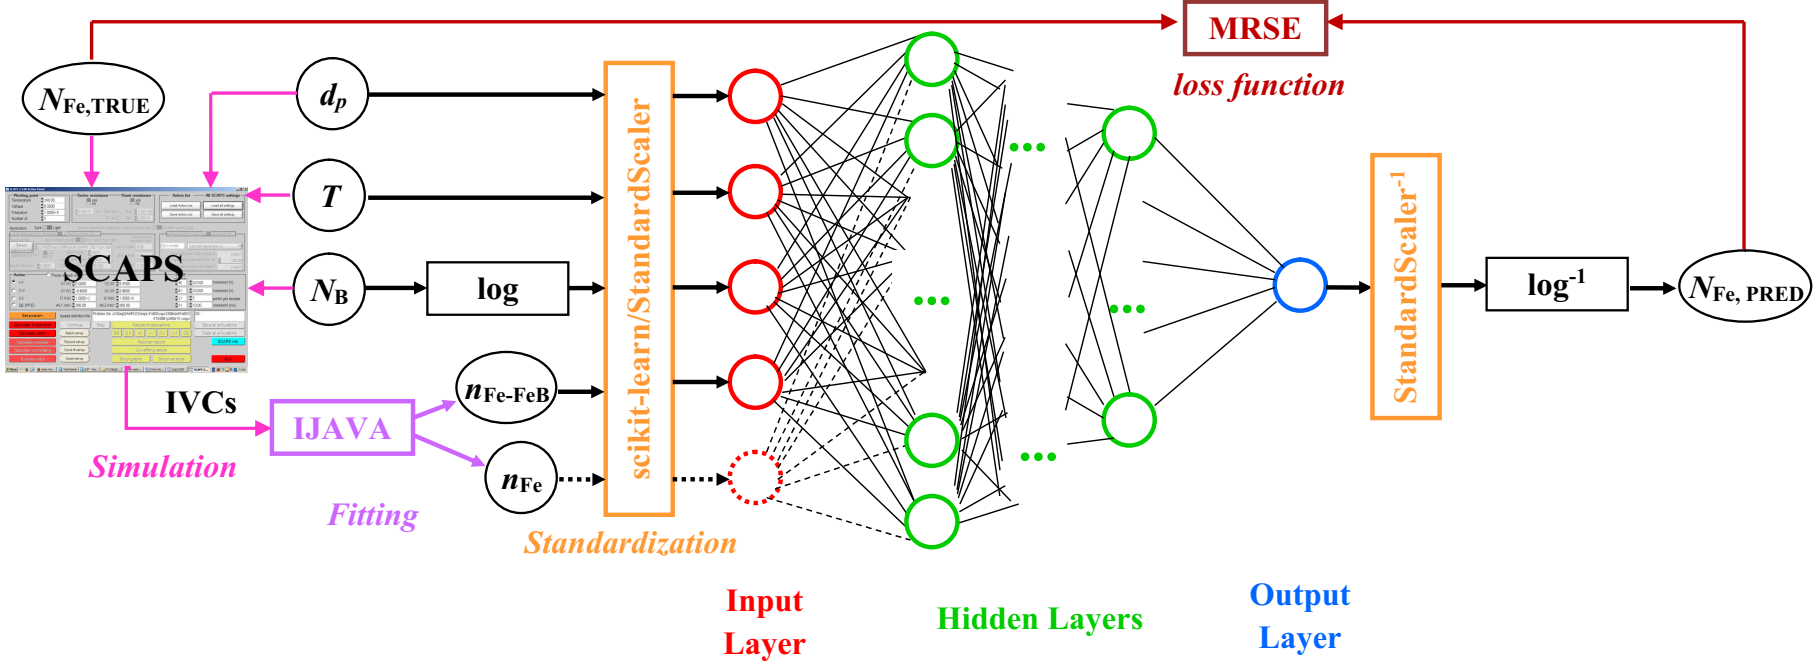
\includegraphics[width=0.8\textwidth]{Chem}
\caption{Scheme of deep learning-based approach for predicting iron concentration.
Additional details are discussed in the body of the article.
}
\label{fig_chem}
\end{figure}


\section{Simulation Details}

The $n^+$--$p$--$p^+$ structure used in calculations
had 0.5~$\mu$m thick emitter layer $n^+$ with donor concentration $N_D=10^{19}$~cm$^{-3}$;
the $p$-layer and $p^+$-layer were uniformly doped with boron;
the base $p$ had the thickness $d_p=150$--$240$~$\mu$m
and dopant concentration $N_\mathrm{B}=10^{15}$--$10^{17}$~cm$^{-3}$;
the BSF-layer $p^+$ had the thickness $d_{BSF}$ ($1$~$\mu$m)
and the acceptor concentration $N_{BSF}=5\times10^{18}$~cm$^{-3}$.

The simulations  were carried out over the temperature range $290-340$~K.
For each temperature, the SCAPS setting file was created
by using the following material parameters.
The bandgap $E_G$ and bandgap narrowing $\Delta E_G$ models were taken from
P\"{a}ssler \cite{Pasler} and Yan and Cuevas \cite{EgNarrow} respectively:
\begin{eqnarray}
\label{eqEg}
E_G=E_{G0}-\alpha\Theta\left\{\frac{1-3\Delta^2}{e^{\frac{\Theta}{T}}-1}
    +\frac{3\Delta^2}{2}\left(\sqrt[6]{1+\frac{\pi^2}{3(1+\Delta^2)}\left(\frac{2T}{\Theta}\right)^2
    +\frac{3\Delta^2-1}{4}\left(\frac{2T}{\Theta}\right)^3+\frac{8}{3}\left(\frac{2T}{\Theta}\right)^4
    +\left(\frac{2T}{\Theta}\right)^6}-1\right)\right\}\,,\\
\Delta E_G=4.20\times10^{-5}\left[\ln\left(\frac{N_{D}}{10^{14}}\right)\right]^3\,;\qquad
     \Delta E_G=4.72\times10^{-5}\left[\ln\left(\frac{N_{B,BSF}}{10^{14}}\right)\right]^3\,,
\end{eqnarray}
where
$E_{G0}=1.1701$~eV,
$\alpha=3.23\times10^{-4}$~eV/K,
$\Theta=446$~K,
$\Delta=0.51$.
The carrier thermal velocities were calculated from the model suggested by Green \citep{Nc:Green}:
\begin{equation}
\label{eqVth}
    \upsilon_{\mathrm{th},n}=\sqrt{\frac{8qkT}{0.28m_0\pi}}\,;\qquad
    \upsilon_{\mathrm{th},p}=\sqrt{\frac{8qkT}{0.41m_0\pi}}\,,
\end{equation}
where
$m_0$ is a free electron mass.
The effective state density masses in the conduction band $m^*_{dC}$ and
valence band $m^*_{dV}$ were calculated according to the model from Couderc et al. \citep{Si_ni_Couderc}
\begin{eqnarray}
  \left(\frac{m^*_{dC}}{m_0}\right)^{1.5} &=& 1.094-1.312\times10^{-5}T+6.753\times10^{-7}T^2+4.609\times10^{-10}T^3\,, \\
  \left(\frac{m^*_{dV}}{m_0}\right)^{1.5} &=& 0.3426+3.376\times10^{-3}T-4.689\times10^{-6}T^2+2.525\times10^{-9}T^3\,.
\end{eqnarray}
The carrier mobilities and the free carrier effective masses  were taken from Klaassen \cite{KLAASSEN953}
and O'Mara et al. \cite{OMara}, respectively.
The temperature and doping dependencies of Auger recombination coefficients were calculated from models by Altermatt et al. \cite{Si_Auger}:
\begin{eqnarray}
% \nonumber to remove numbering (before each equation)
   \nonumber C_{p} (T)&=& (7.91\times10^{-32}-4.13\times10^{-35}T+3.59\times10^{-37}T^2)\\
  &&\times\left(1+\left(564812T^{-1.6545}-1\right)\left(1-\tanh\left[\left\{\frac{p}{5\times10^{16}}\right\}^{0.29}\right]\right)\right)\,, \\
   C_{n} (T)&=& 2.8\times10^{-31}
  \times\left(1+\left(235548T^{-1.5013}-1\right)\left(1-\tanh\left[\left\{\frac{n}{5\times10^{16}}\right\}^{0.34}\right]\right)\right)\,.
\end{eqnarray}
The band-to-band radiation recombination coefficient was taken from Nguyen et al. \cite{Si_BtB}.

The outside surface recombination with electron and hole velocities $10^3$~cm/s ware taken into account.
For metal contacts on the rear and front surfaces,
the flat bands' conditions were assumed. 


The simulations were carried out under the assumption that defect–assisted recombination corresponds only to iron–related deep levels.
As the base and SBF-layer are uniform contaminants, iron is assumed to be in concentration
$N_{\mathrm{Fe}}=10^{10}$--$10^{13}$~cm$^{-3}$.
It is known that Fe in silicon can be in two states:
in the form of FeB pair or in the interstitial state Fe$_i$.
At near room temperature and boron concentration $>10^{14}$~cm$^{-3}$,
almost all Fe bound in FeB pairs is in equilibrium \cite{FeB:kinetic,FeBAssJAP2014,FeBAssSST2011,FeBJAP2005}.
According to Wijaranakula\cite{FeB:kinetic},
the concentration of interstitial iron atoms $N_{\mathrm{Fe}_i}$ which
remain unpaired in equilibrium state depend on temperature, doping level,
and Fermi level $F$ position.
The estimations show that at 340~K  $N_{\mathrm{Fe}_i}\simeq0.1 N_\mathrm{Fe}$
for $N_\mathrm{B}\simeq10^{15}$~cm$^{-3}$ in the quasi-neutral
region of SC base.
However, numerous researches show that temporarily dissociation of pairs can be performed either
by heating to the temperature above 200$^\circ$C,
or by applying intense illumination at room temperature \cite{FeBAssJAP2014,FeBJAP2005}.

The simulations were performed for the following two cases.
In the first case, the concentration of totally dissolved iron was given by a sum of
concentrations of interstitial iron atoms $\mathrm{Fe}_i$
and  trigonal iron-boron pairs $\mathrm{Fe}_i\mathrm{B}_s$:
\begin{equation}\label{eqNFeB}
  N_{\mathrm{Fe}}=N_{\mathrm{Fe}_i}+N_{\mathrm{Fe}_i\mathrm{B}_s}\,.
\end{equation}
The defect distributions in base and $p^+$-layer are inhomogeneous, depend on the Fermi level $F$ position, and are given by
\cite{MurphyJAP2011,FeB:kinetic}:
\begin{equation}
\label{eqNFeB}
    \frac{N_{\mathrm{FeB}}}{N_{\mathrm{Fe}}}=\frac{N_\mathrm{B}10^{-23}\exp\left(-\frac{E_b}{kT}\right)}
     {\left[1+\frac{N_\mathrm{B}}{10^{23}}\exp\left(-\frac{E_b}{kT}\right)\right]\left[1+\exp\left(-\frac{F-E_{\mathrm{Fe}_i}}{kT}\right)\right]}\,,
     \quad N_{\mathrm{Fe}_i}=N_{\mathrm{Fe}}-N_{\mathrm{FeB}}\,,
\end{equation}
where
$E_b=0.582$~eV is the binding energy of $\mathrm{Fe}_i\mathrm{B}_s$ pairs,
$E_{\mathrm{Fe}_i}$ is the donor level associated with $\mathrm{Fe}_i$.
This case corresponds to the equilibrium condition and in this article it will be referred to as ``Fe-FeB''.

In the second case, $\mathrm{Fe}_i$ was assumed to be homogeneously distributed ($N_{\mathrm{Fe}_i}=N_{\mathrm{Fe}}$).
This condition can be realized by heat treatment (210$^\circ$C, 3~min) \cite{FeB_Zong}
or intense illumination \cite{FeBLight2}. This case will be referred to as ``Fe''.

The donor level $E_{\mathrm{Fe}_i} = E_V+0.394$~eV
with electron $\sigma_{n,{\mathrm{Fe}}}=3.47\times10^{-11}T^{-1.48}$~cm$^2$ and
hole $\sigma_{p,{\mathrm{Fe}}}=4.54\times10^{-16}\exp\left(-\frac{0.05}{kT}\right)$~cm$^2$ capture cross-sections \cite{MurphyJAP2011,ROUGIEUX2018}
was associated with $\mathrm{Fe}_i$ in our simulations.
For $\mathrm{Fe}_i\mathrm{B}_s$ the donor level $E_{\mathrm{FeB}}^\mathrm{D}= E_V+0.10$~eV,
$\sigma_{n,{\mathrm{FeB}}}^\mathrm{D}=4\times10^{-13}$~cm$^2$,
$\sigma_{p,{\mathrm{FeB}}}^\mathrm{D}=2\times10^{-14}$~cm$^2$
and acceptor level $E_{\mathrm{FeB}}^\mathrm{A}= E_C-0.26$~eV,
$\sigma_{n,{\mathrm{FeB}}}^\mathrm{A}=5.1\times10^{-9}T^{-2.5}$~cm$^2$,
$\sigma_{p,{\mathrm{FeB}}}^\mathrm{A}=3.32\times10^{-10}\exp\left(-\frac{0.262}{kT}\right)$~cm$^2$
\cite{Istratov1999,MurphyJAP2011,ROUGIEUX2018}
were used.

The dark forward IV characteristics were generated by SCAPS over a voltage range to $0.45$~V.
According to the two-diode model, the dark SC current is given by \citep{Breitenstein2013}
\begin{equation}
\label{eqIVd}
    I=I_{01}\left[\exp\left(-\frac{q(V-R_sI)}{kT}\right)-1\right]
      + I_{02}\left[\exp\left(-\frac{q(V-R_sI)}{nkT}\right)-1\right]
      +\frac{V-R_sI}{R_{sh}}\,,
\end{equation}
where
$I_{01}$ and $I_{02}$ are saturation currents,
$R_{sh}$ and $R_s$ are shunt and series resistances.
The two-diode model is often applied to describe real Si SCs:
in Eq.~(\ref{eqIVd}) the first diode represents the ``ideal'' diode
and the first term in the equation describes recombination
in the base depth and emitter, including their surfaces;
the second diode is the so-called recombination diode
and the second term describes recombination within the depletion region \citep{Breitenstein2013}.
The simulated data were fitted by Eq.~(\ref{eqIVd})
with $n$, $I_{01}$, $I_{02}$,
$R_{sh}$, and $R_s$ as fitting parameters.
The fitting was performed by meta--heuristic method IJAVA \cite{IJAVA}.
The typical example of IV curves and fitting results is shown
in Supplementary Material.
It should be noted that
i)~the influence of both $R_s$ (obtained values $<10^{-2}$~$\Omega$) and $R_{sh}$
(obtained values $>10^{18}$~$\Omega$) can be neglected in the simulated IVs;
ii)~the contribution of recombination diode current is essential at low bias only
and the voltage range $(0-0.45)$~V is quite sufficient
to determine the ideality factor values accurately.

In our further calculations we used the ideality factors
obtained in  Fe-case and Fe-FeB-case
which are referred to as  $n_\mathrm{Fe}$ and $n_\mathrm{Fe-FeB}$ hereafter.
The typical simulated dependencies of  the ideality factor are shown in Fig.~\ref{fig_nValues}
and in Supplementary Material.
The detailed discussion about $n_\mathrm{Fe}$ and $n_\mathrm{Fe-FeB}$ values are presented elsewhere \cite{OlikhJPS},
however it should be noted that
(i)~$n$ can be the same for different  values of SC parameters;
(ii)~dependencies of $n_\mathrm{Fe}$ and $n_\mathrm{Fe-FeB}$ differ not only in absolute values but also in behavior, although insignificantly.

\begin{figure}[t]
\centering
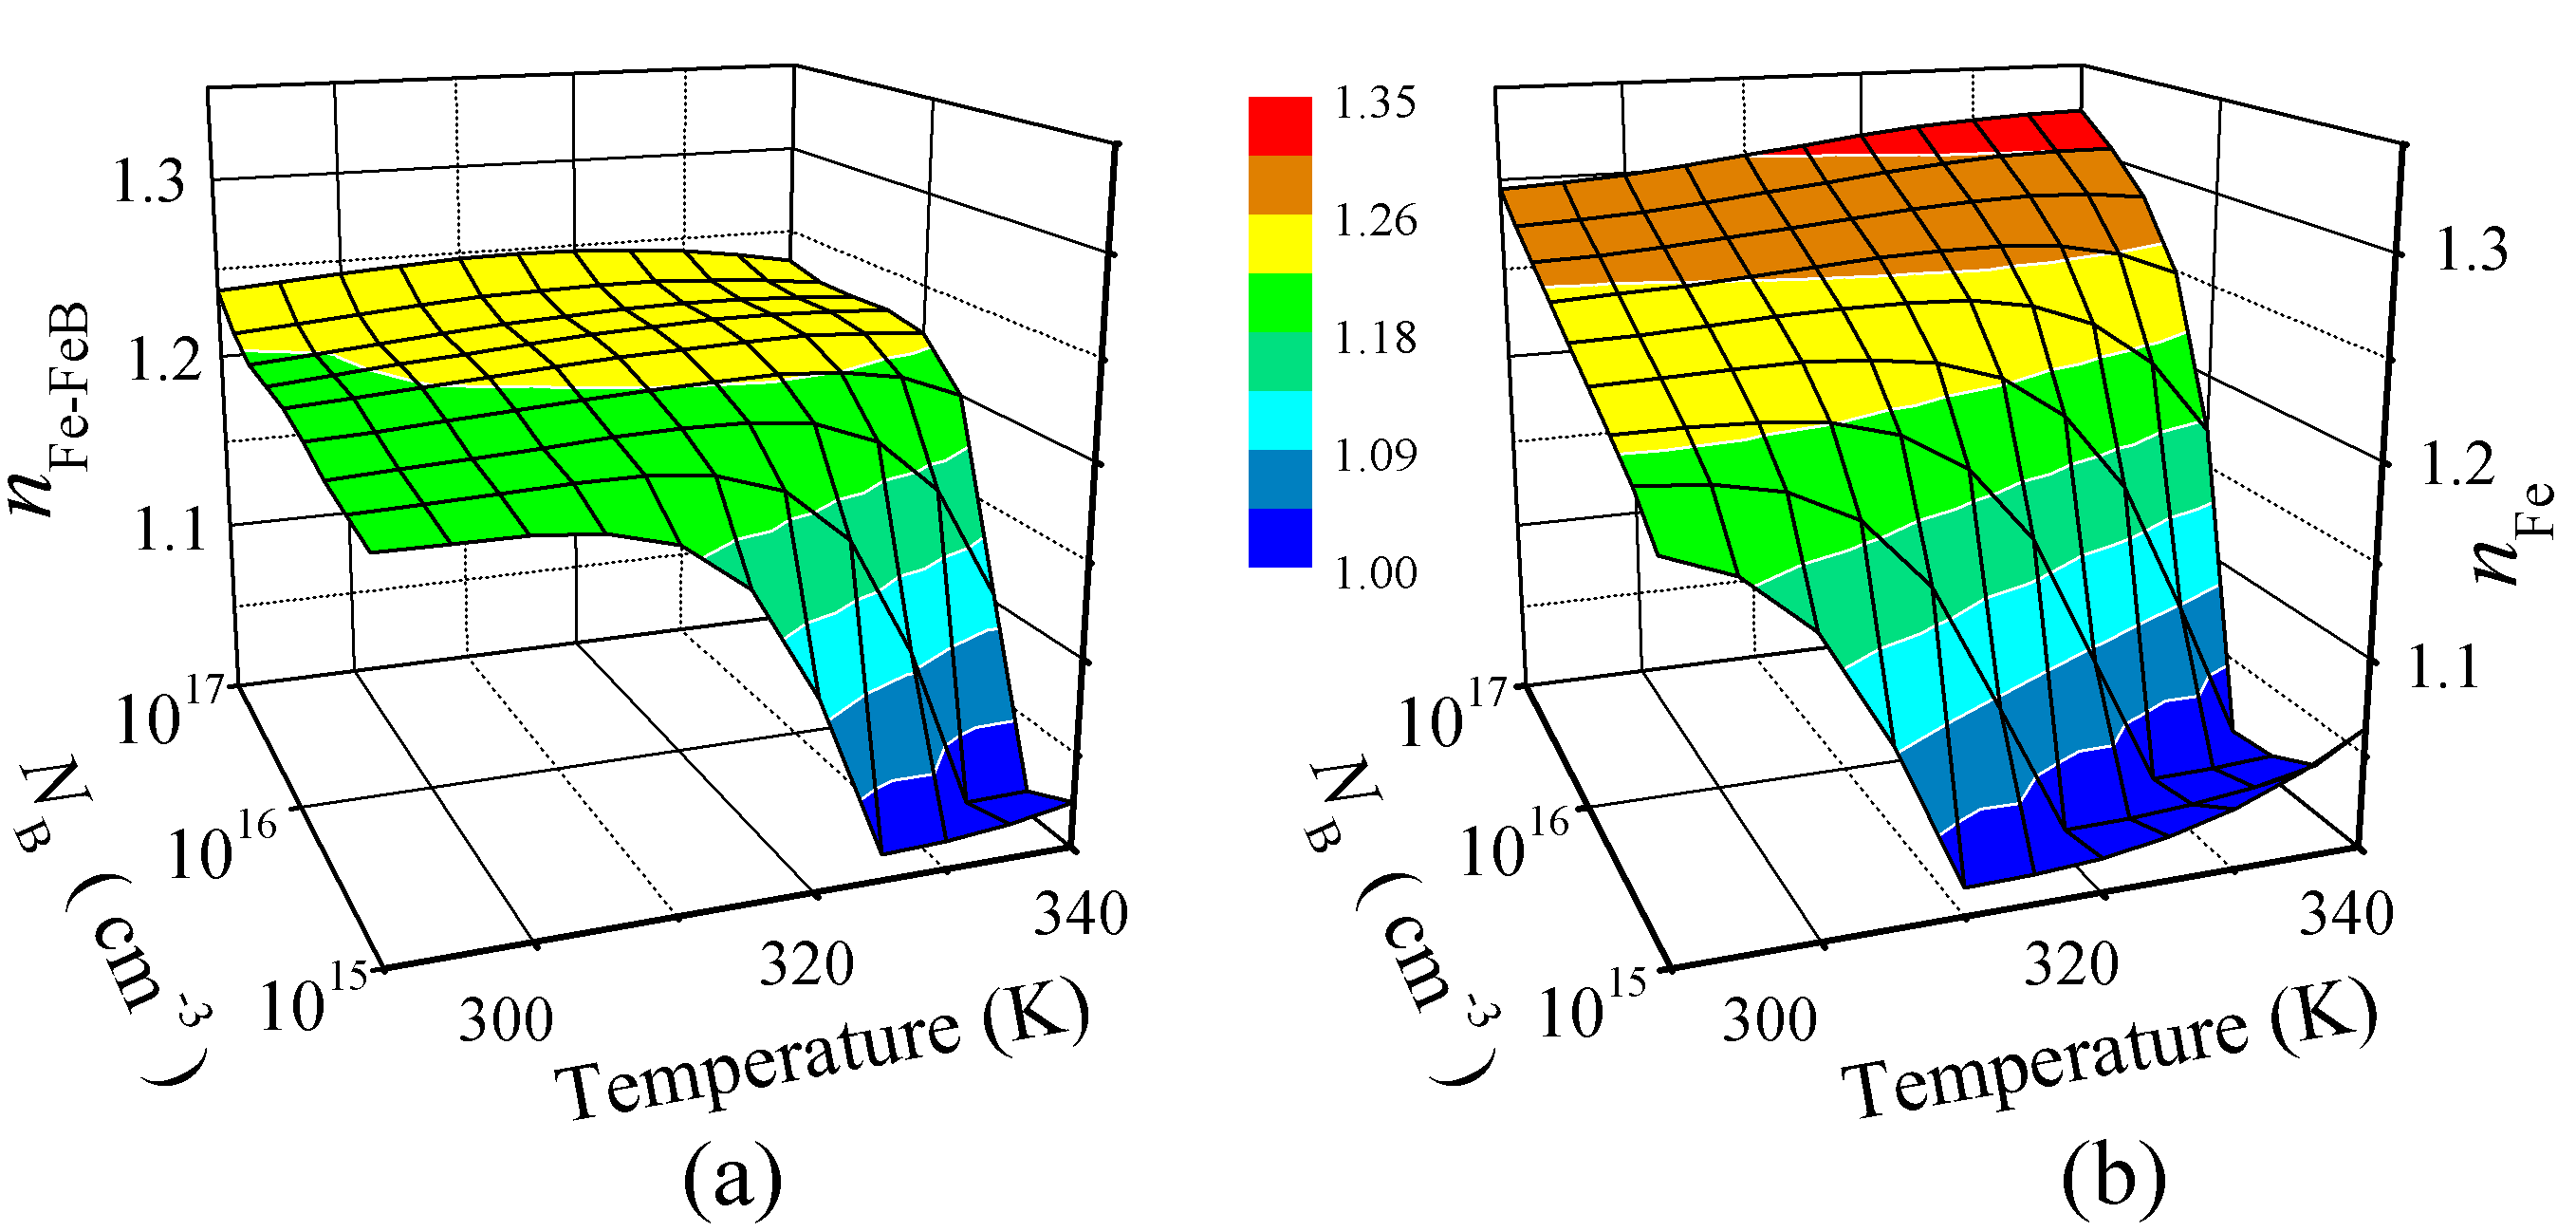
\includegraphics[width=0.48\textwidth]{Fig1a}
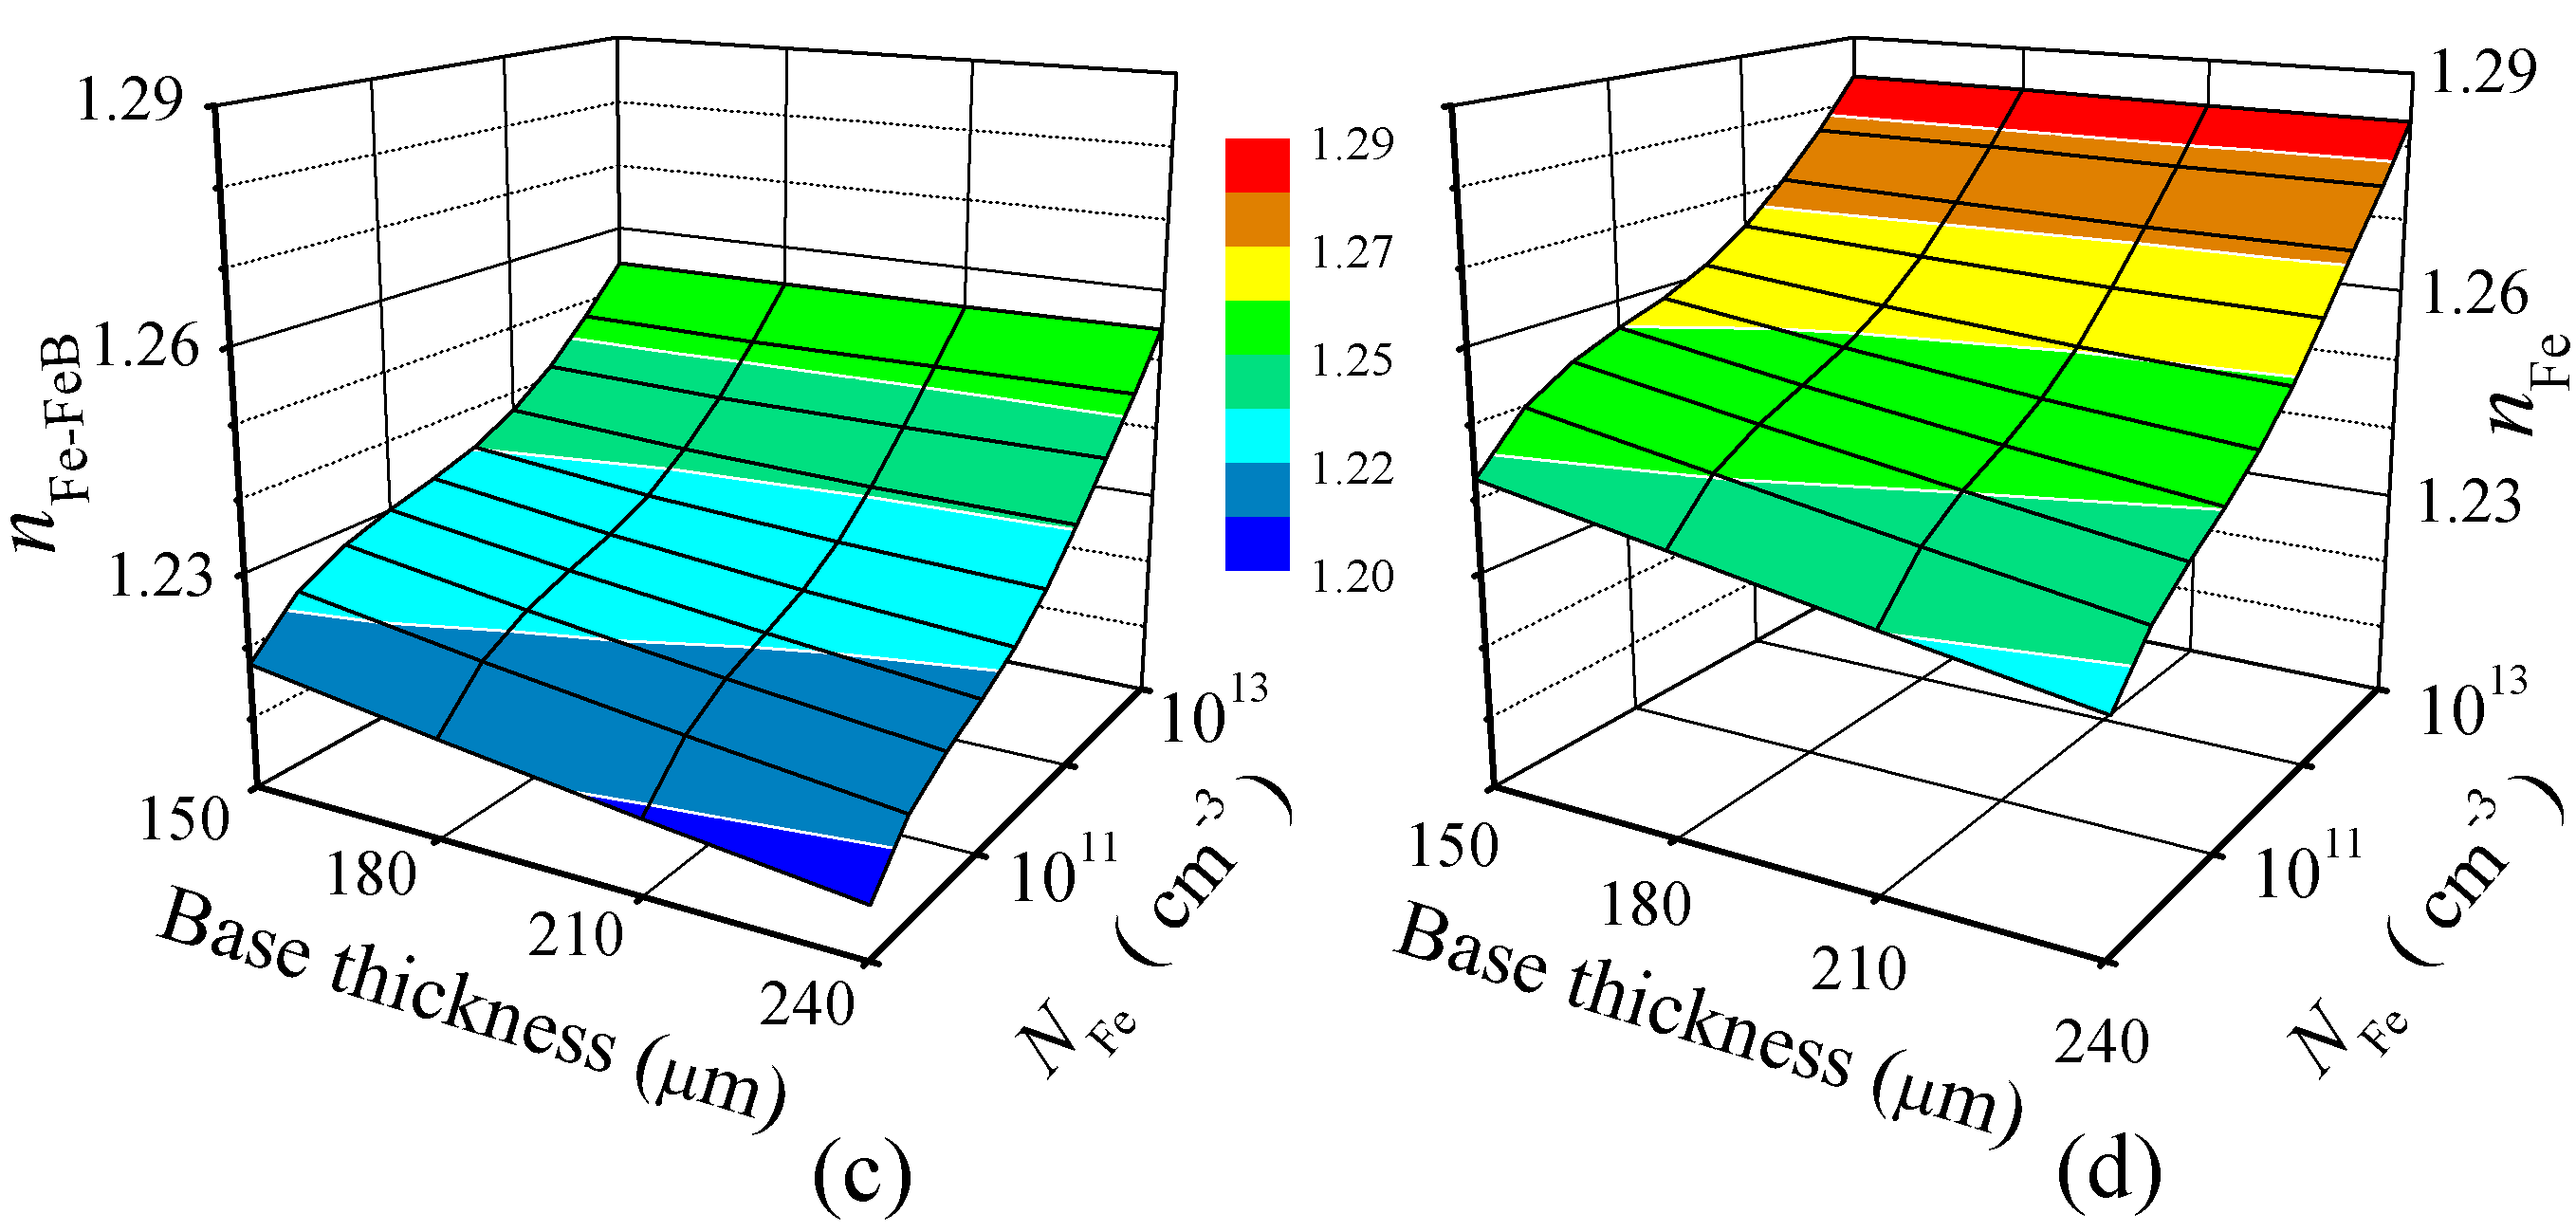
\includegraphics[width=0.48\textwidth]{Fig1b}
\caption{Ideality factor versus temperature and boron concentration (a, b)
or base thickness and iron concentration (c,d).
The Fe-FeB-case (a, c) and Fe-case (b, d).
$N_\mathrm{Fe}=10^{10}$~cm$^{-3}$ (a,b),
$d_p=180$~$\mu$m (a, b),
$N_\mathrm{B}=10^{16}$~cm$^{-3}$ (c, d),
$T=320$~K (c, d).
}
\label{fig_nValues}
\end{figure}

\section{Deep neural network models}

Deep neural network training  requires a large number of samples.
In order to build a training dataset, we used IV characteristics
simulated by using 4 $d_p$ values, 9 $N_\mathrm{B}$ values, 11 $T$ values, and 19 $N_{\mathrm{Fe}}$ values
which are regularly distributed
(for $T$ and $d_p$ in linear scale,
for  $N_{\mathrm{Fe}}$ and $N_\mathrm{B}$ in logarithmic scale)
over the  ranges $150$--$240$~$\mu$m, $10^{15}$--$10^{17}$~cm$^{-3}$, $290-340$~K, and
$10^{10}$--$10^{13}$~cm$^{-3}$, respectively.
Therefore, 7524 IV characteristics were simulated in Fe-case and in Fe-FeB-case.



In addition, several test datasets were prepared.
For instance, the test dataset labeled ``Fe-varied'' consists of two subsets.
The $N_{\mathrm{Fe}}$ values
$1.300\times10^{10}$, $2.471\times10^{10}$, $4.696\times10^{10}$,
$8.927\times10^{10}$, $1.697\times10^{11}$, $3.225\times10^{11}$,
$6.130\times10^{11}$, $1.165\times10^{120}$, $2.214\times10^{12}$,
$4.209\times10^{12}$, $8.000\times10^{12}$~cm$^{-3}$
(not used during training dataset creation),
$T$ values 290, 295, 300, 305, 310, 315, 320, 325, 330, 335, 340~K
(used during training dataset creation),
$d_p$ value 180~$\mu$m (used during training dataset creation),
and $N_\mathrm{B}$ values
$1.778\times10^{15}$, $5.623\times10^{15}$, $10^{16}$,
$3.162\times10^{16}$, $10^{17}$~cm$^{-3}$
(used during training dataset creation)
were used to prepare the first subset.
Thus, the first subset is based on 605 pairs of IV characteristics.
The $N_{\mathrm{Fe}}$ values
$1.200\times10^{110}$, $2.234\times10^{11}$, $4.160\times10^{11}$,
$7.746\times10^{11}$, $1.442\times10^{12}$, $2.685\times10^{12}$,
$5.000\times10^{12}$~cm$^{-3}$
(not used during training dataset creation),
$T$ values 290, 300, 310, 320, 330, 340~K
(used during training dataset creation),
$d_p$ values 210, 240~$\mu$m (used during training dataset creation),
and $N_\mathrm{B}$ values
$3.162\times10^{15}$, $10^{16}$,
$10^{17}$~cm$^{-3}$
(used during training datset creation)
were used to prepare the second subset of Fe-varied test dataset.
Thus, Fe-varied test dataset is based on $605+252=857$~pairs of IV characteristics.

The similar approach was used to prepare ``d-varied'' (1189 samples), ``T-varied'' (832 samples), and ``B-varied'' (514 samples) test datasets.
The base thickness, doping level, temperature, and iron concentration values
which are different from those in training dataset values were used to prepare ``All-varied'' dataset (684 samples).

The precise values of parameters are listed in Supplementary Material.

We have tried to construct a DNN that could estimate iron contamination by using
SC parameters ($d_p$ and $N_\mathrm{B}$), measured temperatures, and the result of IV fitting (the ideality factor).
As shown in Fig.~\ref{fig_chem}, two DNNs with different input parameters are under consideration.
The input sample of the first DNN consists of $\{d_p,\log N_\mathrm{B},T,n_\mathrm{Fe-FeB}\}$.
In practice, this input set can be obtained from one dark IV measurement.
This neural network is referred to as DNN$_\mathrm{FeFeB}$ hereafter.
The second DNN uses  $\{d_p,\log N_\mathrm{B},T,n_\mathrm{Fe-FeB},n_\mathrm{Fe}\}$ in the input layer.
In practice, to obtain a set like this additional SC processing (e.g., intense illumination) and two IV measurements are required.
Further on this neural network is referred to as DNN$_\mathrm{FeFeB-Fe}$.


The dense deep neural network was implemented through a high-level Keras API provided by TensorFlow \cite{Keras}.
The input layers consist of four or five nodes --- see Fig.~\ref{fig_chem}.
In the output layer, one node and linear activation were used.
The five configurations of the hidden layers  were considered:
(i)~``pipe'': each hidden layer contains equal number of nodes;
(ii)~``trapezium'': six hidden layers, number of neurons linearly decreases from 100\% (first layer) to 50\% (last layer);
(iii)~``triangle'': ten layers, number of neurons linearly decreases from 100\% (first layer) to 10\% (last layer);
(iv)~``butterfly'': two serial reflected trapezium configurations;
(v)~``fir'': two serial trapezium configurations.


The mean squared relative error (MSRE) was chosen as the loss function:
\begin{equation}
\label{eqMSRE}
    \mathrm{MSRE}=\frac{1}{N_s}\sum_{i=1}^{N_s}\frac{(N_\mathrm{Fe,TRUE,i}-N_\mathrm{Fe,PRED,i})^2}{N_\mathrm{Fe,TRUE,i}\cdot N_\mathrm{Fe,PRED,i}}\,,
\end{equation}
where
$N_s$ is the number of samples in dataset,
$N_\mathrm{Fe,TRUE,i}$ is the iron concentration used in the $i$--th sample simulation, and
$N_\mathrm{Fe,PRED,i}$ is the DNN prediction for the $i$--th sample.

Hyperparameters include the number of nodes for the first hidden layer,
the number of hidden layers (in pipe configuration),
the batch size,
the activation function,
the optimizer,
the learning rate,
the preprocessing method,
the dropout rate,
the regularization function,
the regularization rate,
and the weight initializer.
The grid search (coarse tuning to limit one hyperparameter) and random search (fine tuning) were performed over the predefined hyperparameter space
shown in Table~\ref{tabHP} and the best hyperparameter combination was chosen.


\begin{table}%[width=\linewidth,cols=2,pos=h]
\caption{Hyperparameter space for DNNs.}\label{tabHP}
\begin{tabular}{ll}%{\tblwidth}{@{} LL@{} }
\headrow
\thead{Hyperparameter}& \thead{Values}\\
%Hyperparameter & Values\\
%\midrule
\# nodes for first
hidden layer & 30, 40, 50, 75, 100, 120, 150 \\
\# hidden layers & 4, 5, 6, 8, 10, 15 \\
 batch size & 8, 16, 32, 64, 128 \\
activation function & ReLu, sigmoid, tanh, SELU, ELU \\
optimizer & SGD, RMSprop, Adam, Adadelta, Adagrad, Adamax, Nadam, Ftrl \\
learning rate & $10^{-5}$, $10^{-4}$, $10^{-3}$, $10^{-2}$\\
\# epochs & 100, 300, 400, 600, 1000, 1500\\
preprocessing method & StandartScaler, MinMaxScaler \\
regularization function& None, L2, L1, Dropout\\
regularization rate & $10^{-5}$, $10^{-4}$, $10^{-3}$, $10^{-2}$\\
dropout rate & 0.2, 0.3, 0.4, 0.5 \\
weight initializer& Xavier Normal or Uniform, He Normal or Uniform, Random Normal or Uniform, Ones\\
\hline
\end{tabular}
\end{table}

To estimate DNN training, 10--fold cross--validation was used.
The performance of the DNN models on test datasets was evaluated by using three metrics:
MSRE, coefficient of determination $R^2$, and coefficient of correlation $R$.
Finally, to increase the DNNs performance, a full dataset consisting of training dataset and all the test datasets  was used for training of the models.

\section{Results and Discussion}
\subsection{Synthetic IV curves}

The results of hyperparameter search are listed in Table~\ref{tabChosenHP}.
In particular,
for DNN$_\mathrm{FeFeB}$ and DNN$_\mathrm{FeFeB-Fe}$
the trapezium and pipe configurations are chosen, respectively.


\begin{table}%[width=.9\linewidth,cols=3,pos=h]
\caption{Chosen hyperparameter combinations.}\label{tabChosenHP}
\begin{tabular}{lll}%{\tblwidth}{@{} LLL@{} }
\headrow
\thead{Hyperparameter} & \thead{DNN$_\mathrm{FeFeB}$}&\thead{DNN$_\mathrm{FeFeB-Fe}$}\\
\# nodes for hidden layers & 120, 108, 96, 84, 72, 60& 100, 100, 100, 100 \\
 batch size & 32 &32 \\
activation function & ReLu & ELU \\
optimizer & Adamax & Adamax\\
learning rate & $10^{-3}$& $10^{-3}$\\
\# epochs & 400 & 1500\\
preprocessing method & StandartScaler& StandartScaler\\
regularization function& None& None\\
weight initializer& Xavier Normal & Xavier Normal\\
\hline
\end{tabular}
\end{table}


The training and test results of DNN$_\mathrm{FeFeB}$ are presented in Table~\ref{table_CV},
Table~\ref{table_MSRE}, and Fig.~\ref{fig_TrDNN1}.
As seen, MSRE of prediction by DNN$_\mathrm{FeFeB}$ is sufficiently large.
However, it should be noted that
in most cases the predictions with big differences between $N_\mathrm{Fe,TRUE,i}$ and $N_\mathrm{Fe,PRED,i}$ are not numerous.
In particular, squared relative error (SRE) does not exceed 0.05 for 87\%, 88\%, and 96\% samples in
T-varied, d-varied and Fe-varid datasets respectively --- see bars in Fig.~\ref{fig_TrDNN1}.
In the case of B-varied dataset (with doping level value non--used in the training dataset),
the biggest $\mathrm{MSRE}=1.06$  is associated with those not often  samples that have a really great SRE (>20)
while  SRE is less than 0.05 for 54\% samples.
The worst predictions are quite expectedly to be observed for the All-varied dataset:
$R^2$ equals 0.813 and SRE$<0.05$ for only 18\% samples.
On the other hand, the Fe-varied dataset is most similar to real situation and
the determination and correlation coefficients are high enough (0.991 and 0.996) in this case.

\begin{table}%[width=.9\linewidth,cols=3,pos=h]
\caption{Results of 10--fold cross--validation}\label{table_CV}
\begin{tabular}{lcc}%{\tblwidth}{@{} LLL@{} }
\headrow
\thead{Dataset} & \multicolumn{2}{c}{MSRE}\\
\headrow
 & \thead{DNN$_\mathrm{FeFeB}$}&\thead{DNN$_\mathrm{FeFeB-Fe}$}\\
training&$0.31\pm0.07$&$0.03\pm0.01$ \\
full&$0.28\pm0.05$& $0.03\pm0.01$\\
\hline
\end{tabular}
\end{table}


\begin{table}%[width=.9\linewidth,cols=7,pos=h]
\caption{DNN's testing results}\label{table_MSRE}
\begin{tabular}{lcccccc}%{\tblwidth}{@{} LLLLLLL@{} }
\headrow
\thead{Dataset} & \multicolumn{3}{c}{DNN$_\mathrm{FeFeB}$}& \multicolumn{3}{c}{DNN$_\mathrm{FeFeB-Fe}$}\\
\headrow
 & \thead{MSRE} & \thead{$R^2$}& \thead{$R$} & \thead{MSRE} & \thead{$R^2$}& \thead{$R$}\\
T--varied&0.41 &0.936 &0.967 & 0.020& 0.994&0.997 \\
d--varied&0.37 &0.961&0.980& 0.018&0.996&0.998\\
B--varied&1.06&0.881&0.939& 0.084&0.991&0.995\\
Fe--varied&0.06 &0.991&0.996& 0.005&0.999&0.999\\
All--varied&0.54 &0.813&0.901& 0.138&0.948&0.974\\
\hline
\end{tabular}
\end{table}

\begin{figure}[tb]
\centering
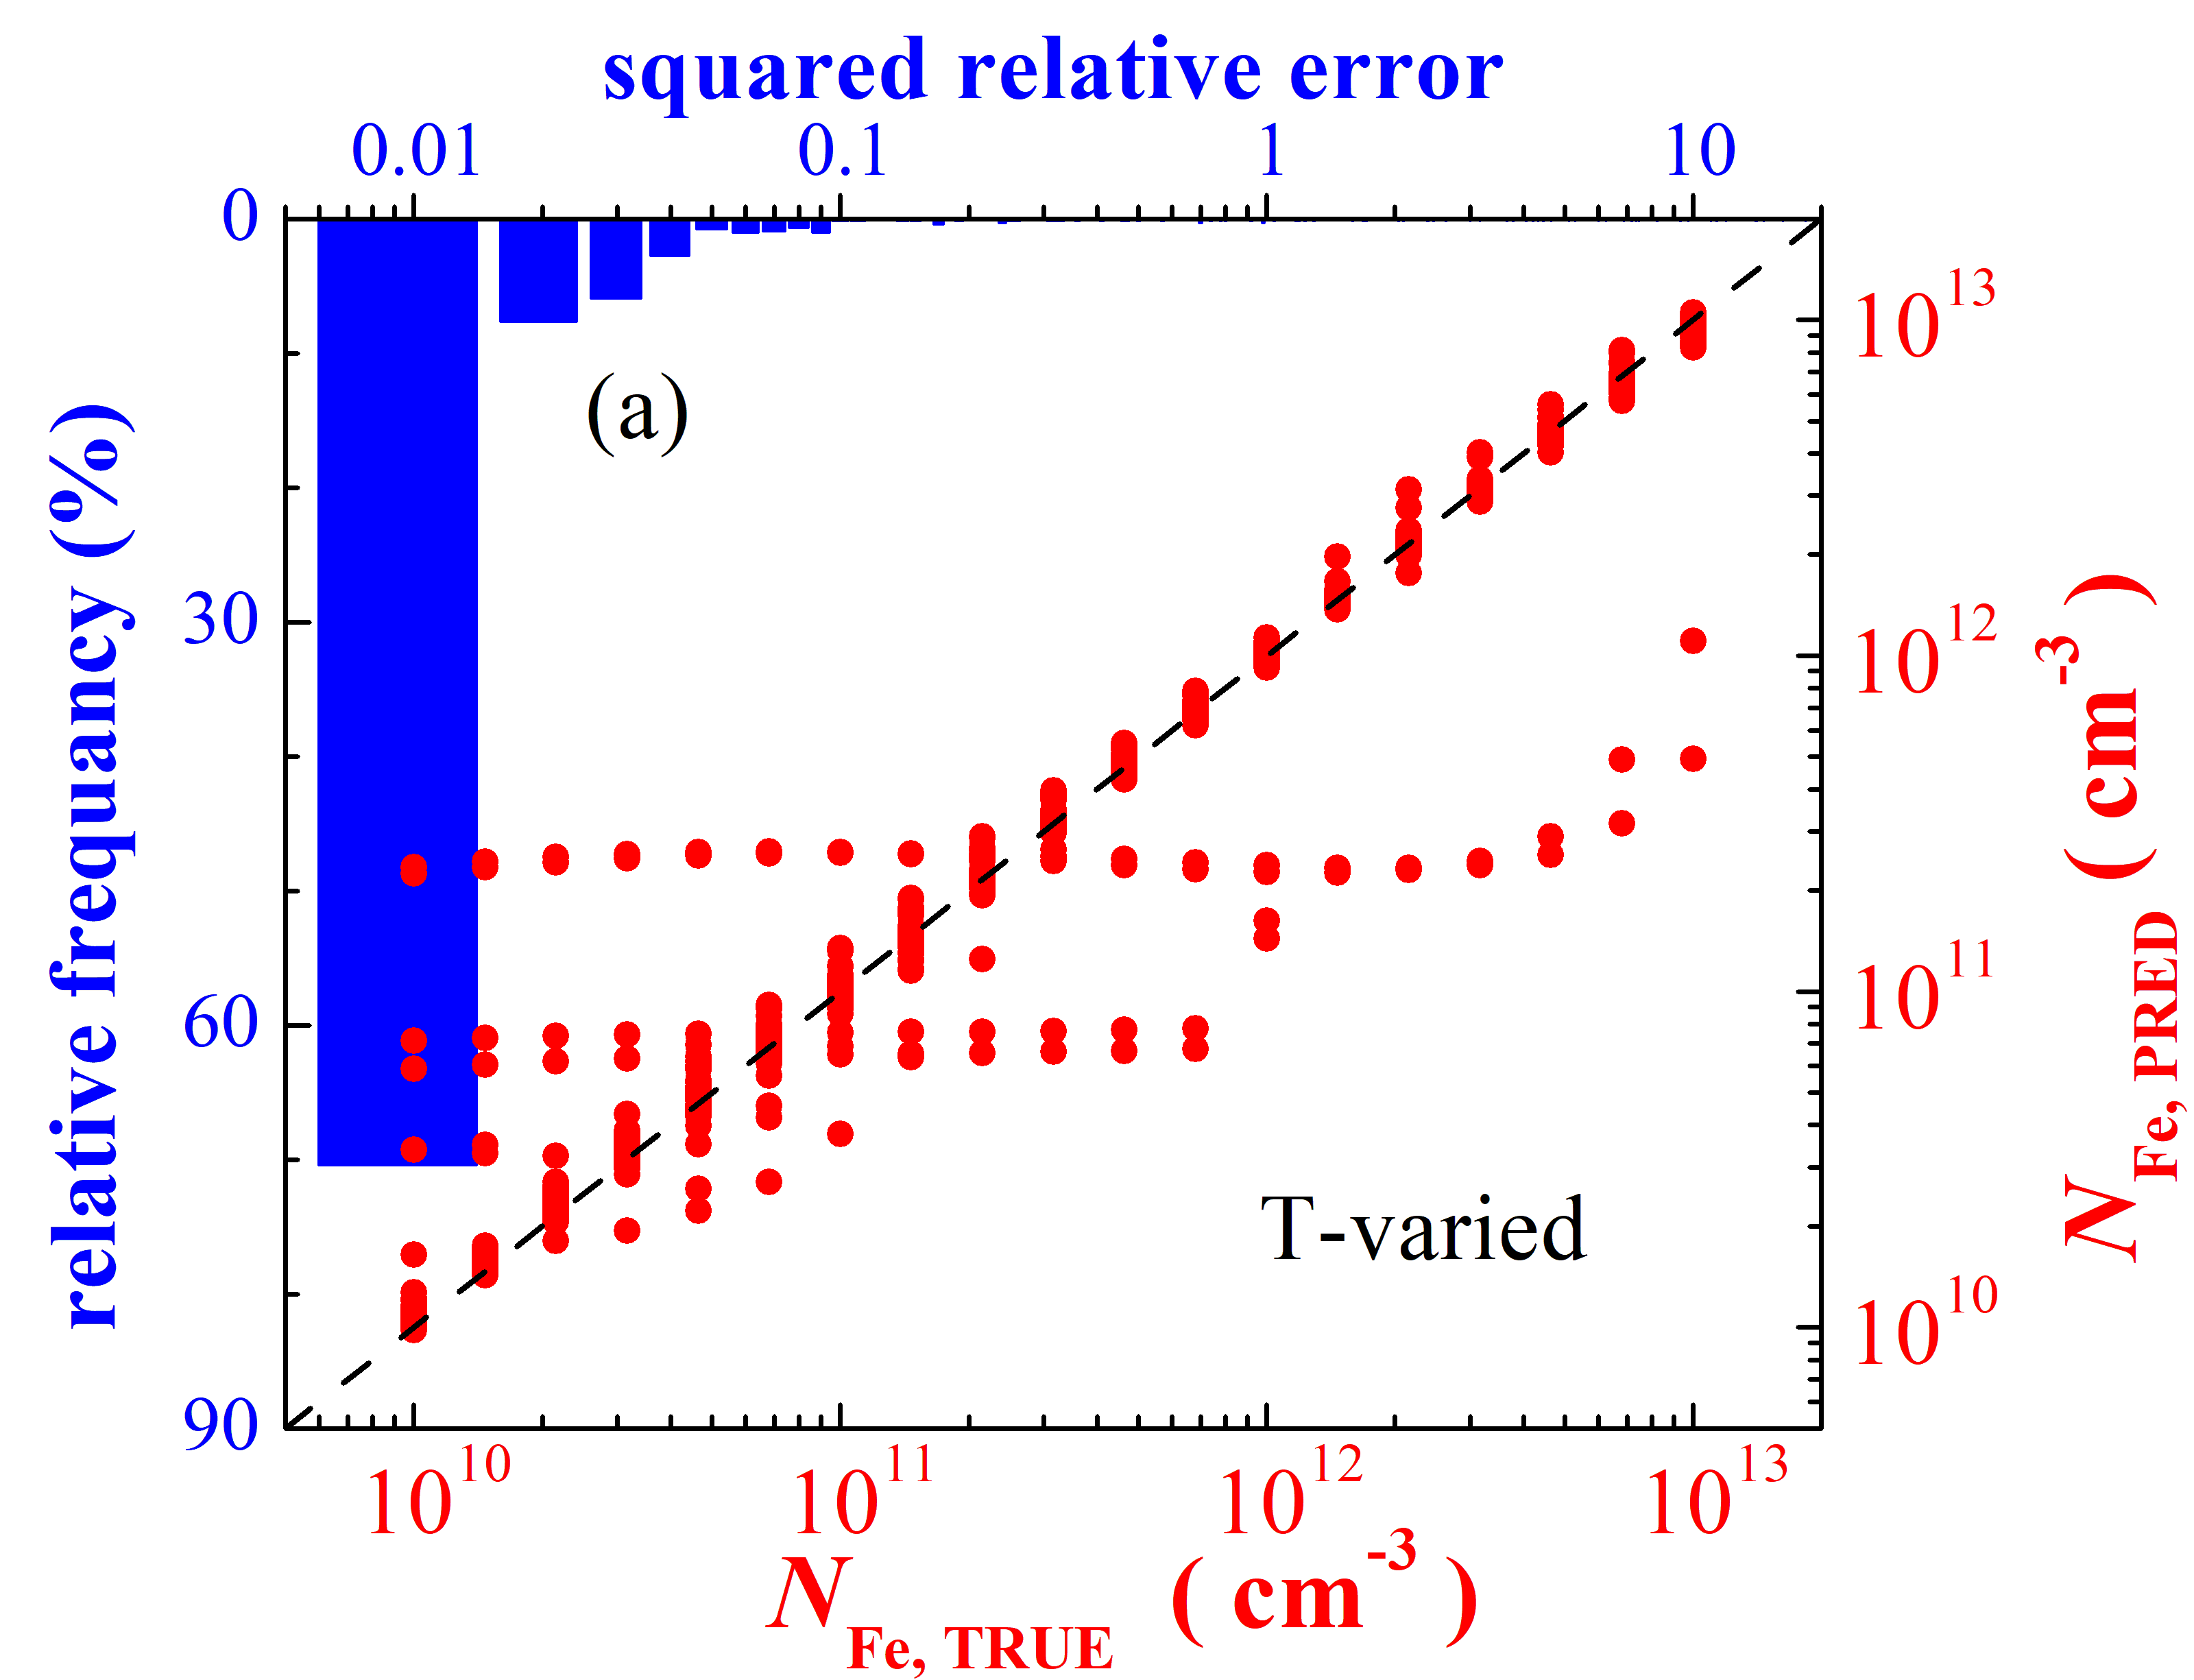
\includegraphics[width=0.32\textwidth]{F3a}
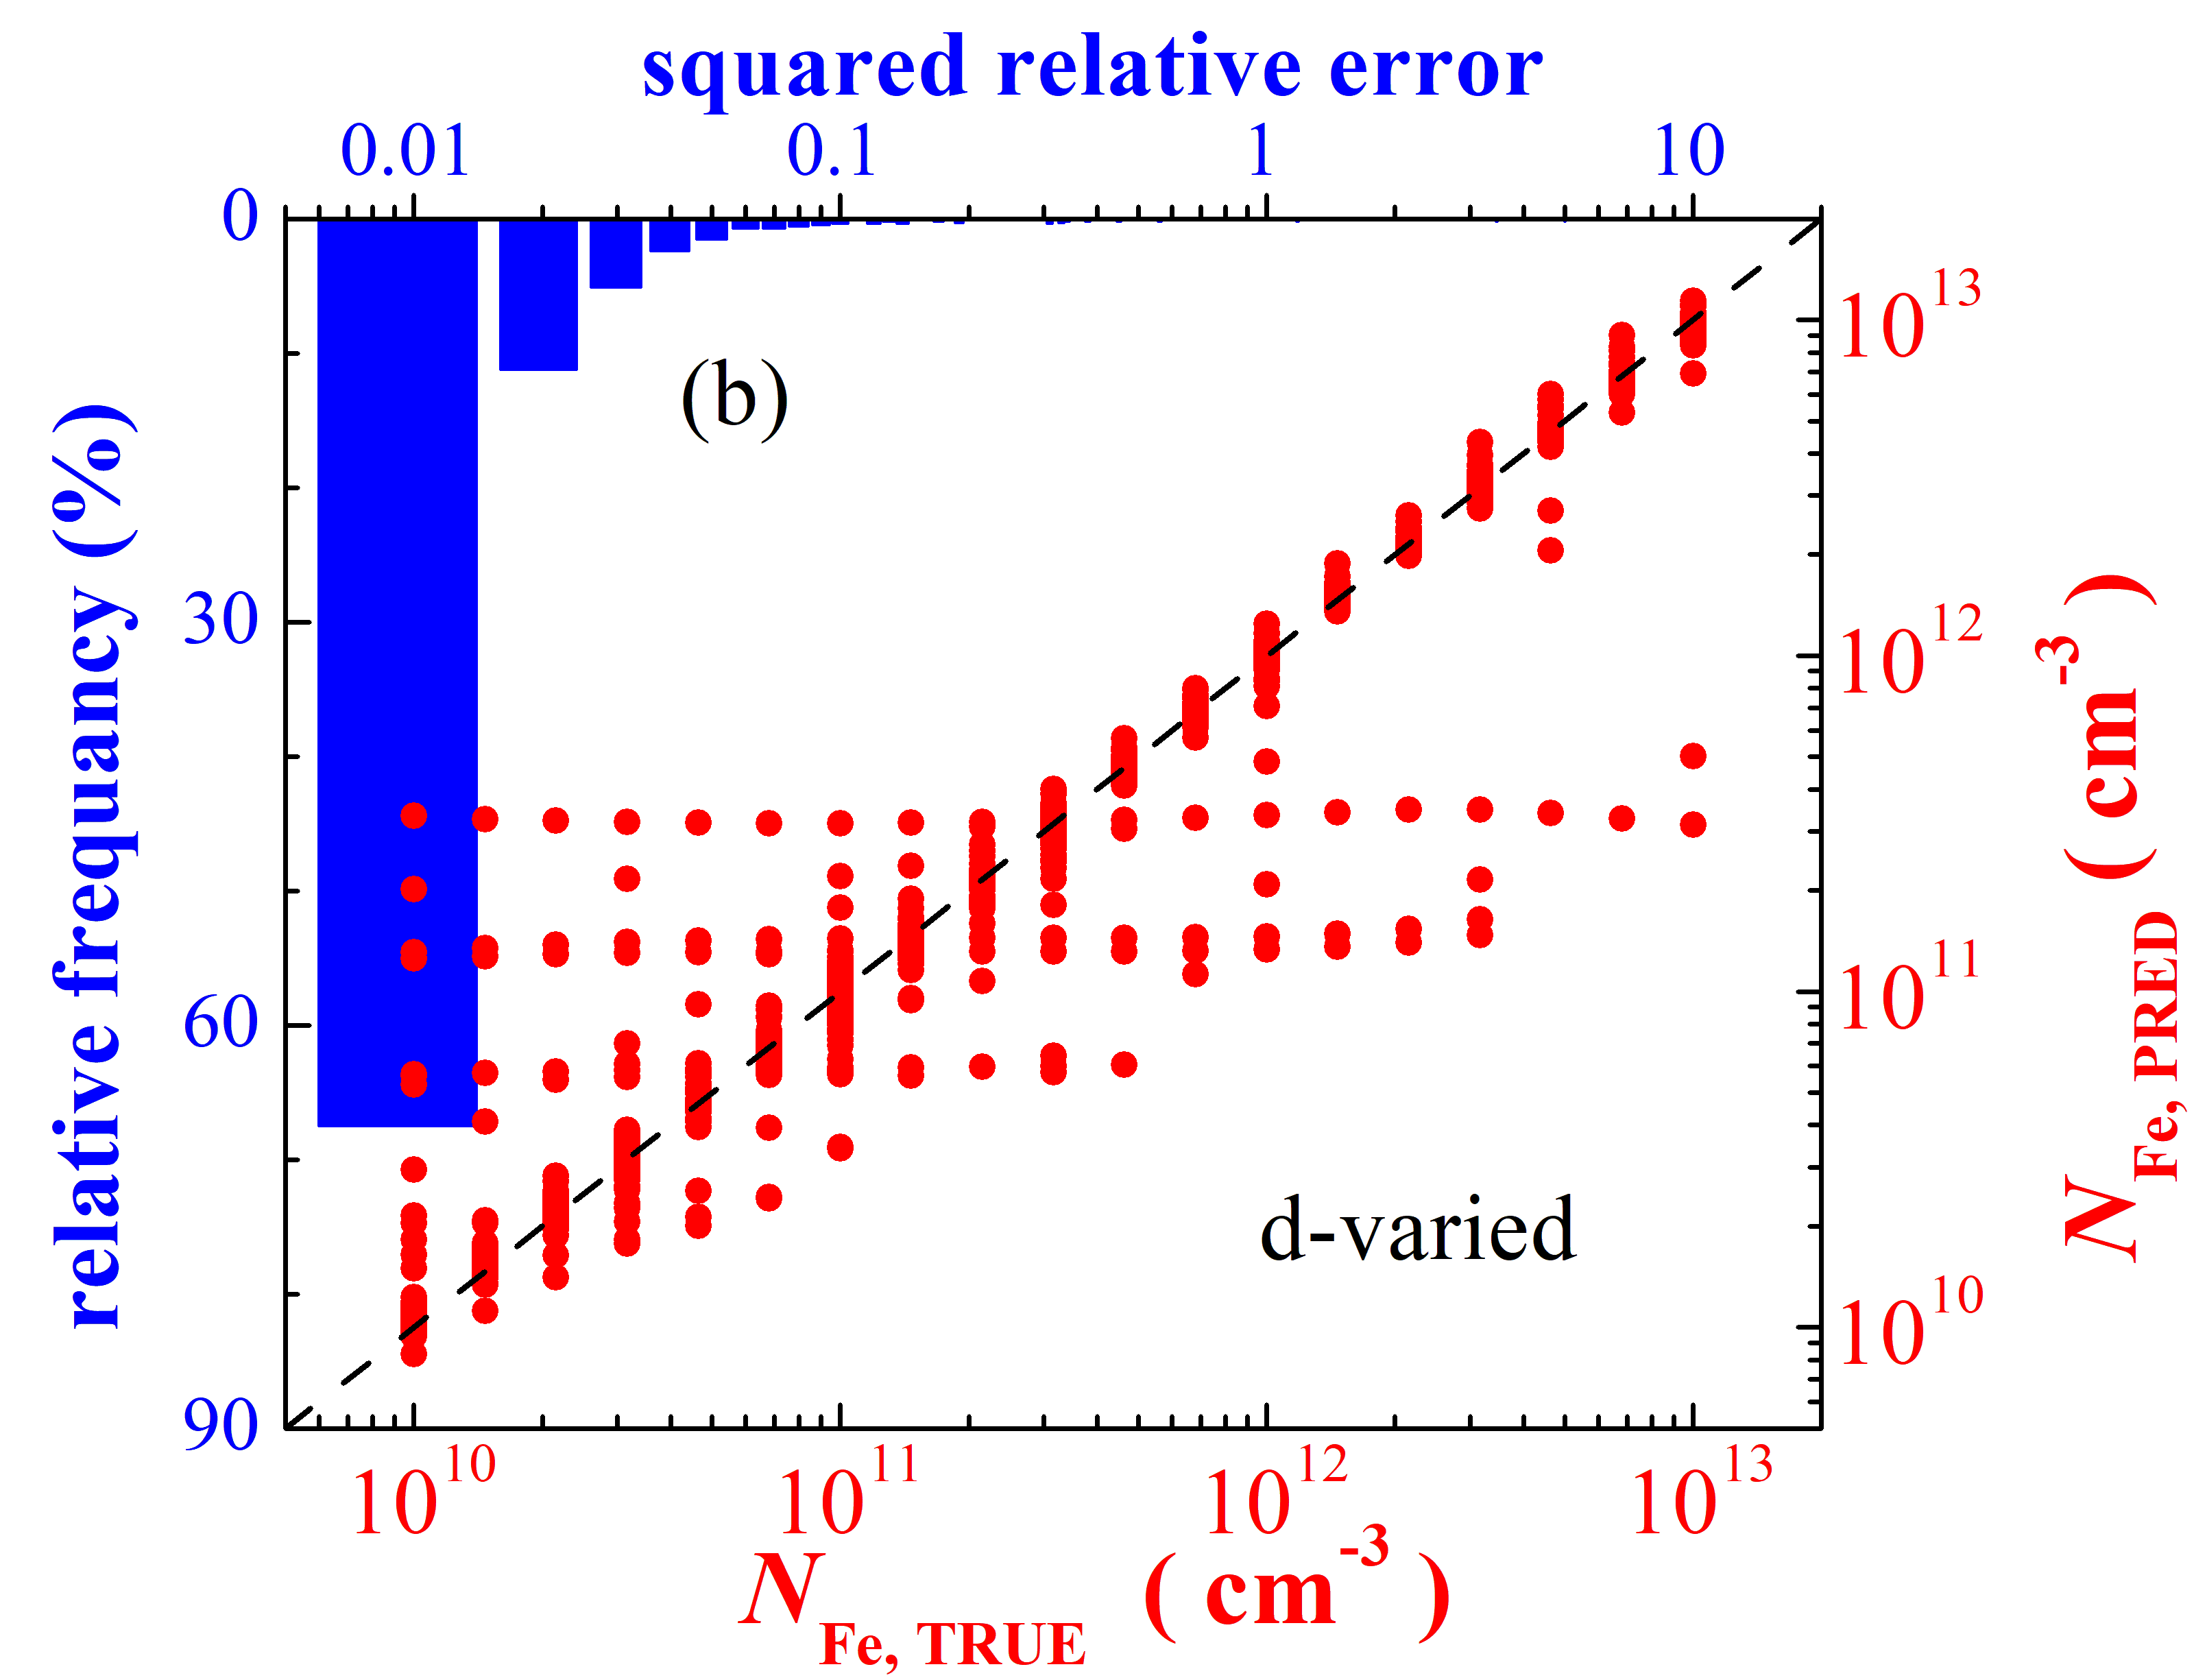
\includegraphics[width=0.32\textwidth]{F3b}
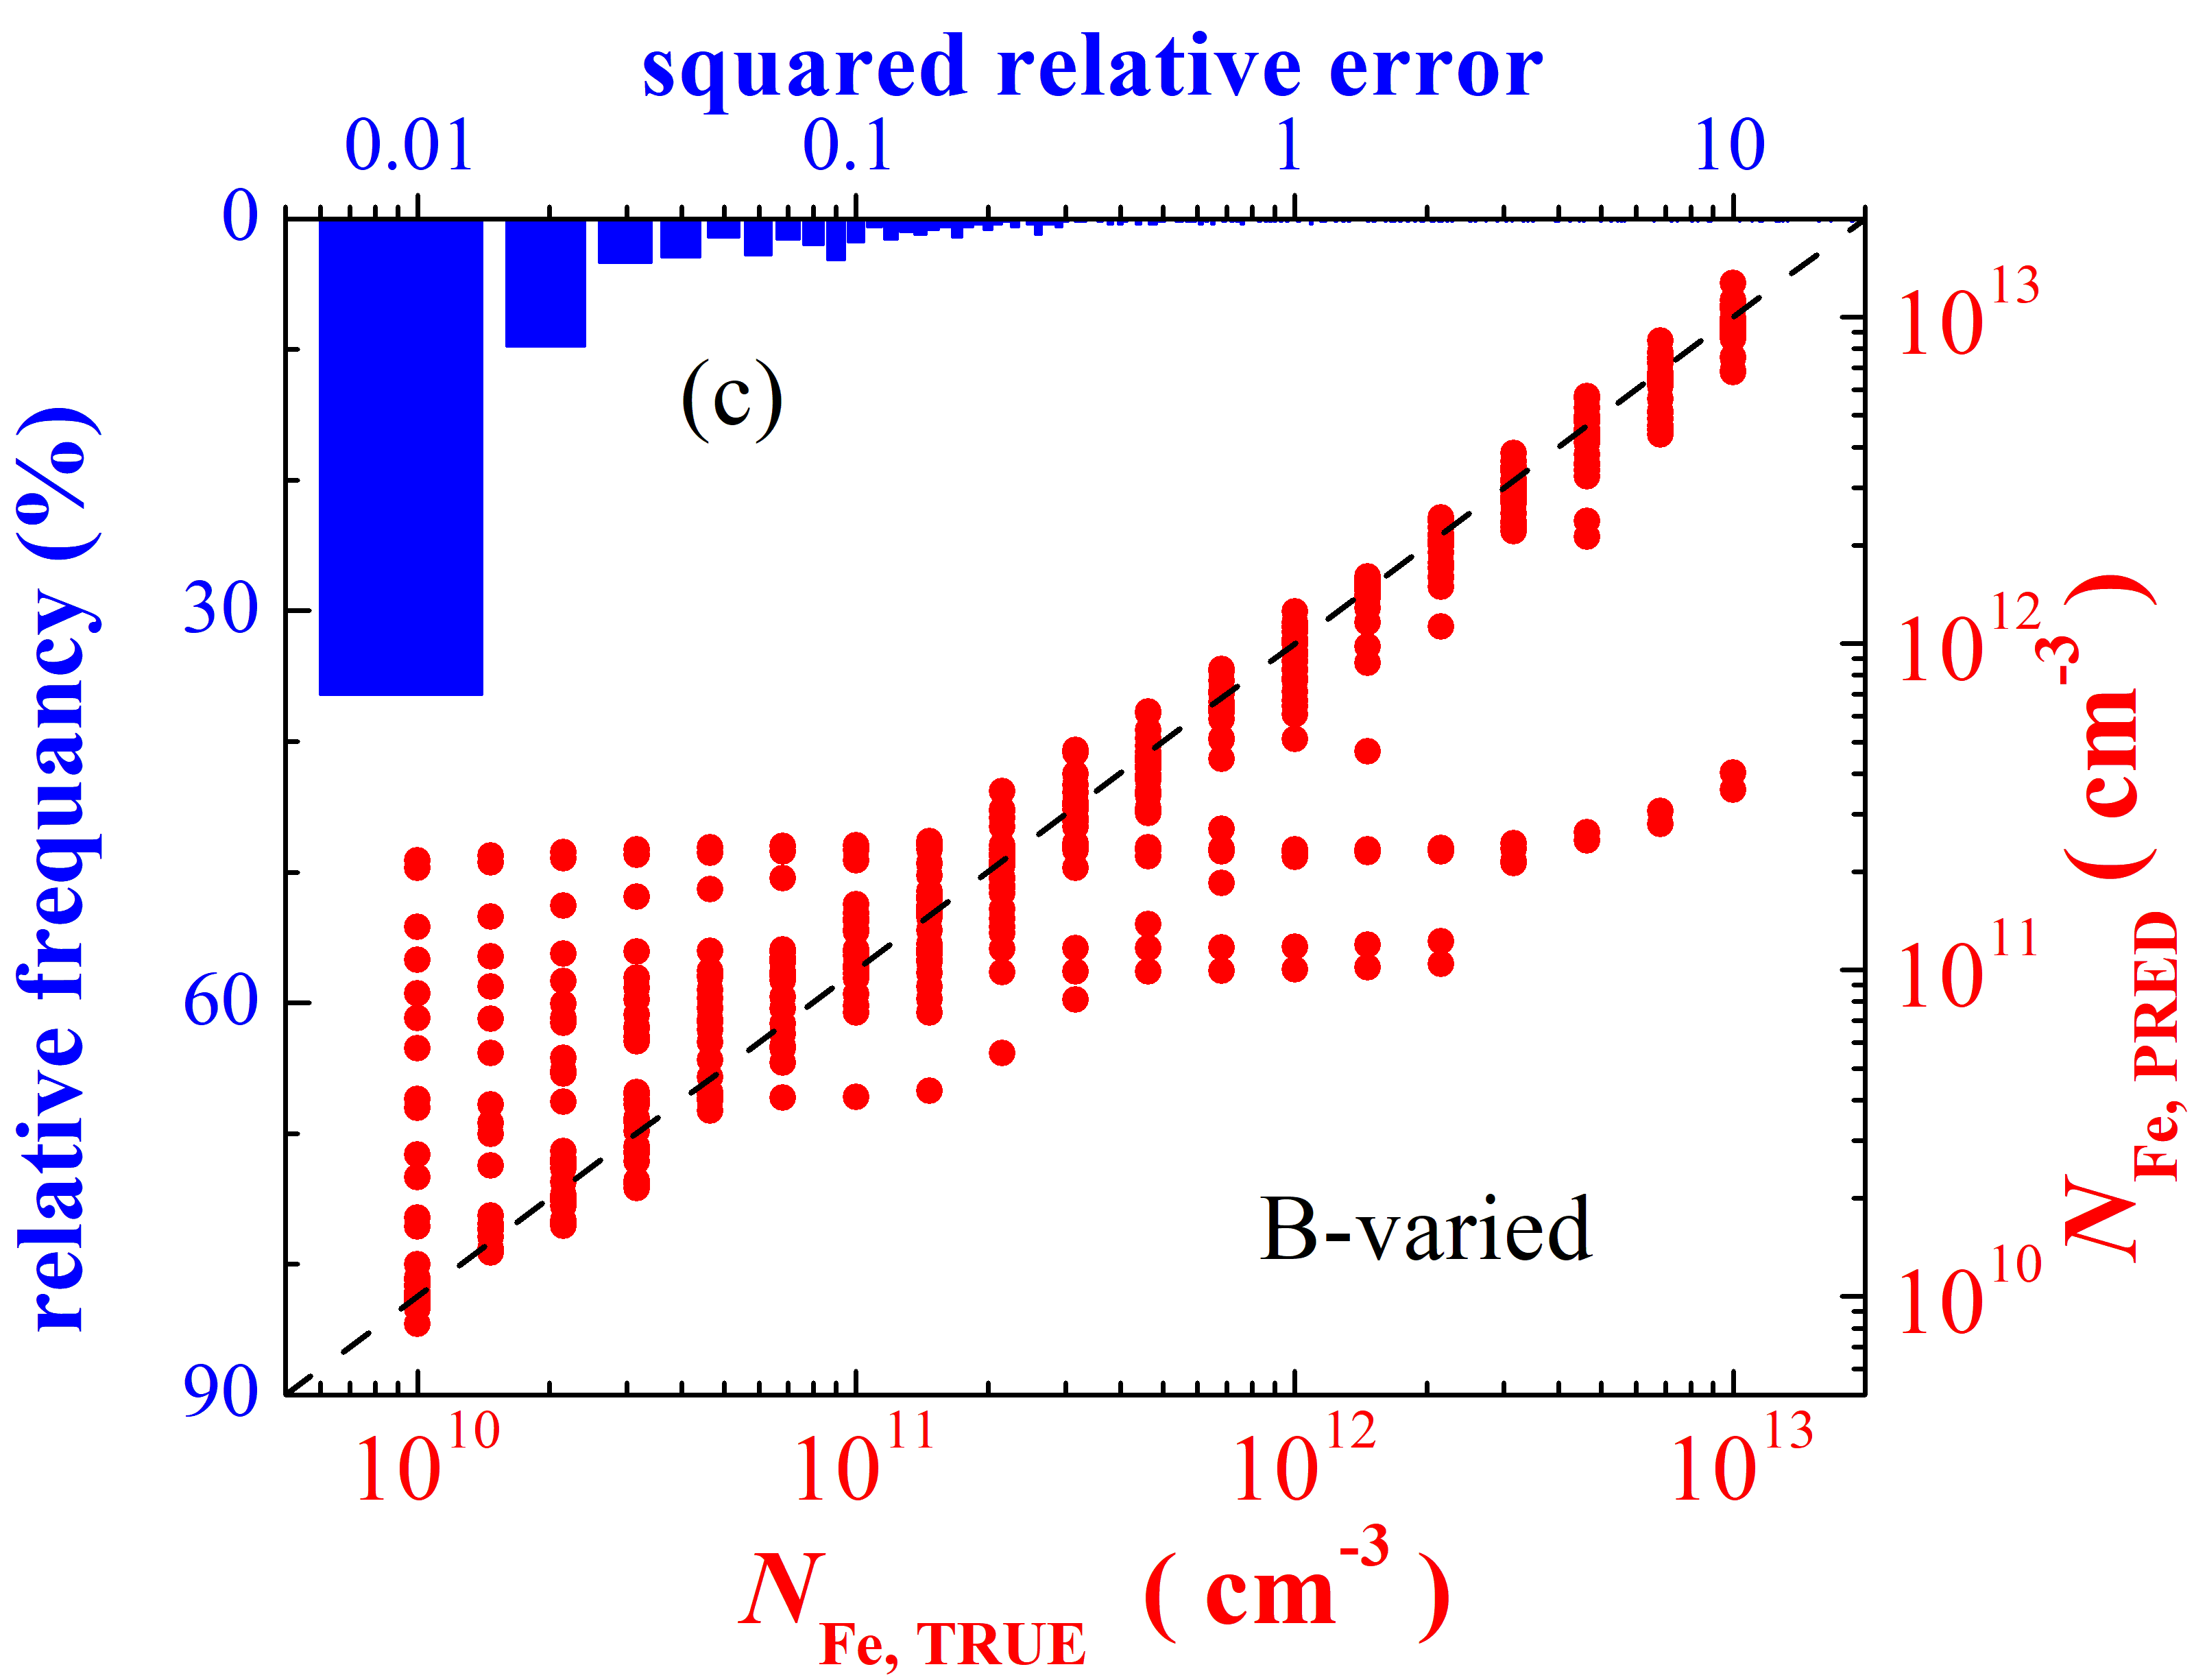
\includegraphics[width=0.32\textwidth]{F3c}
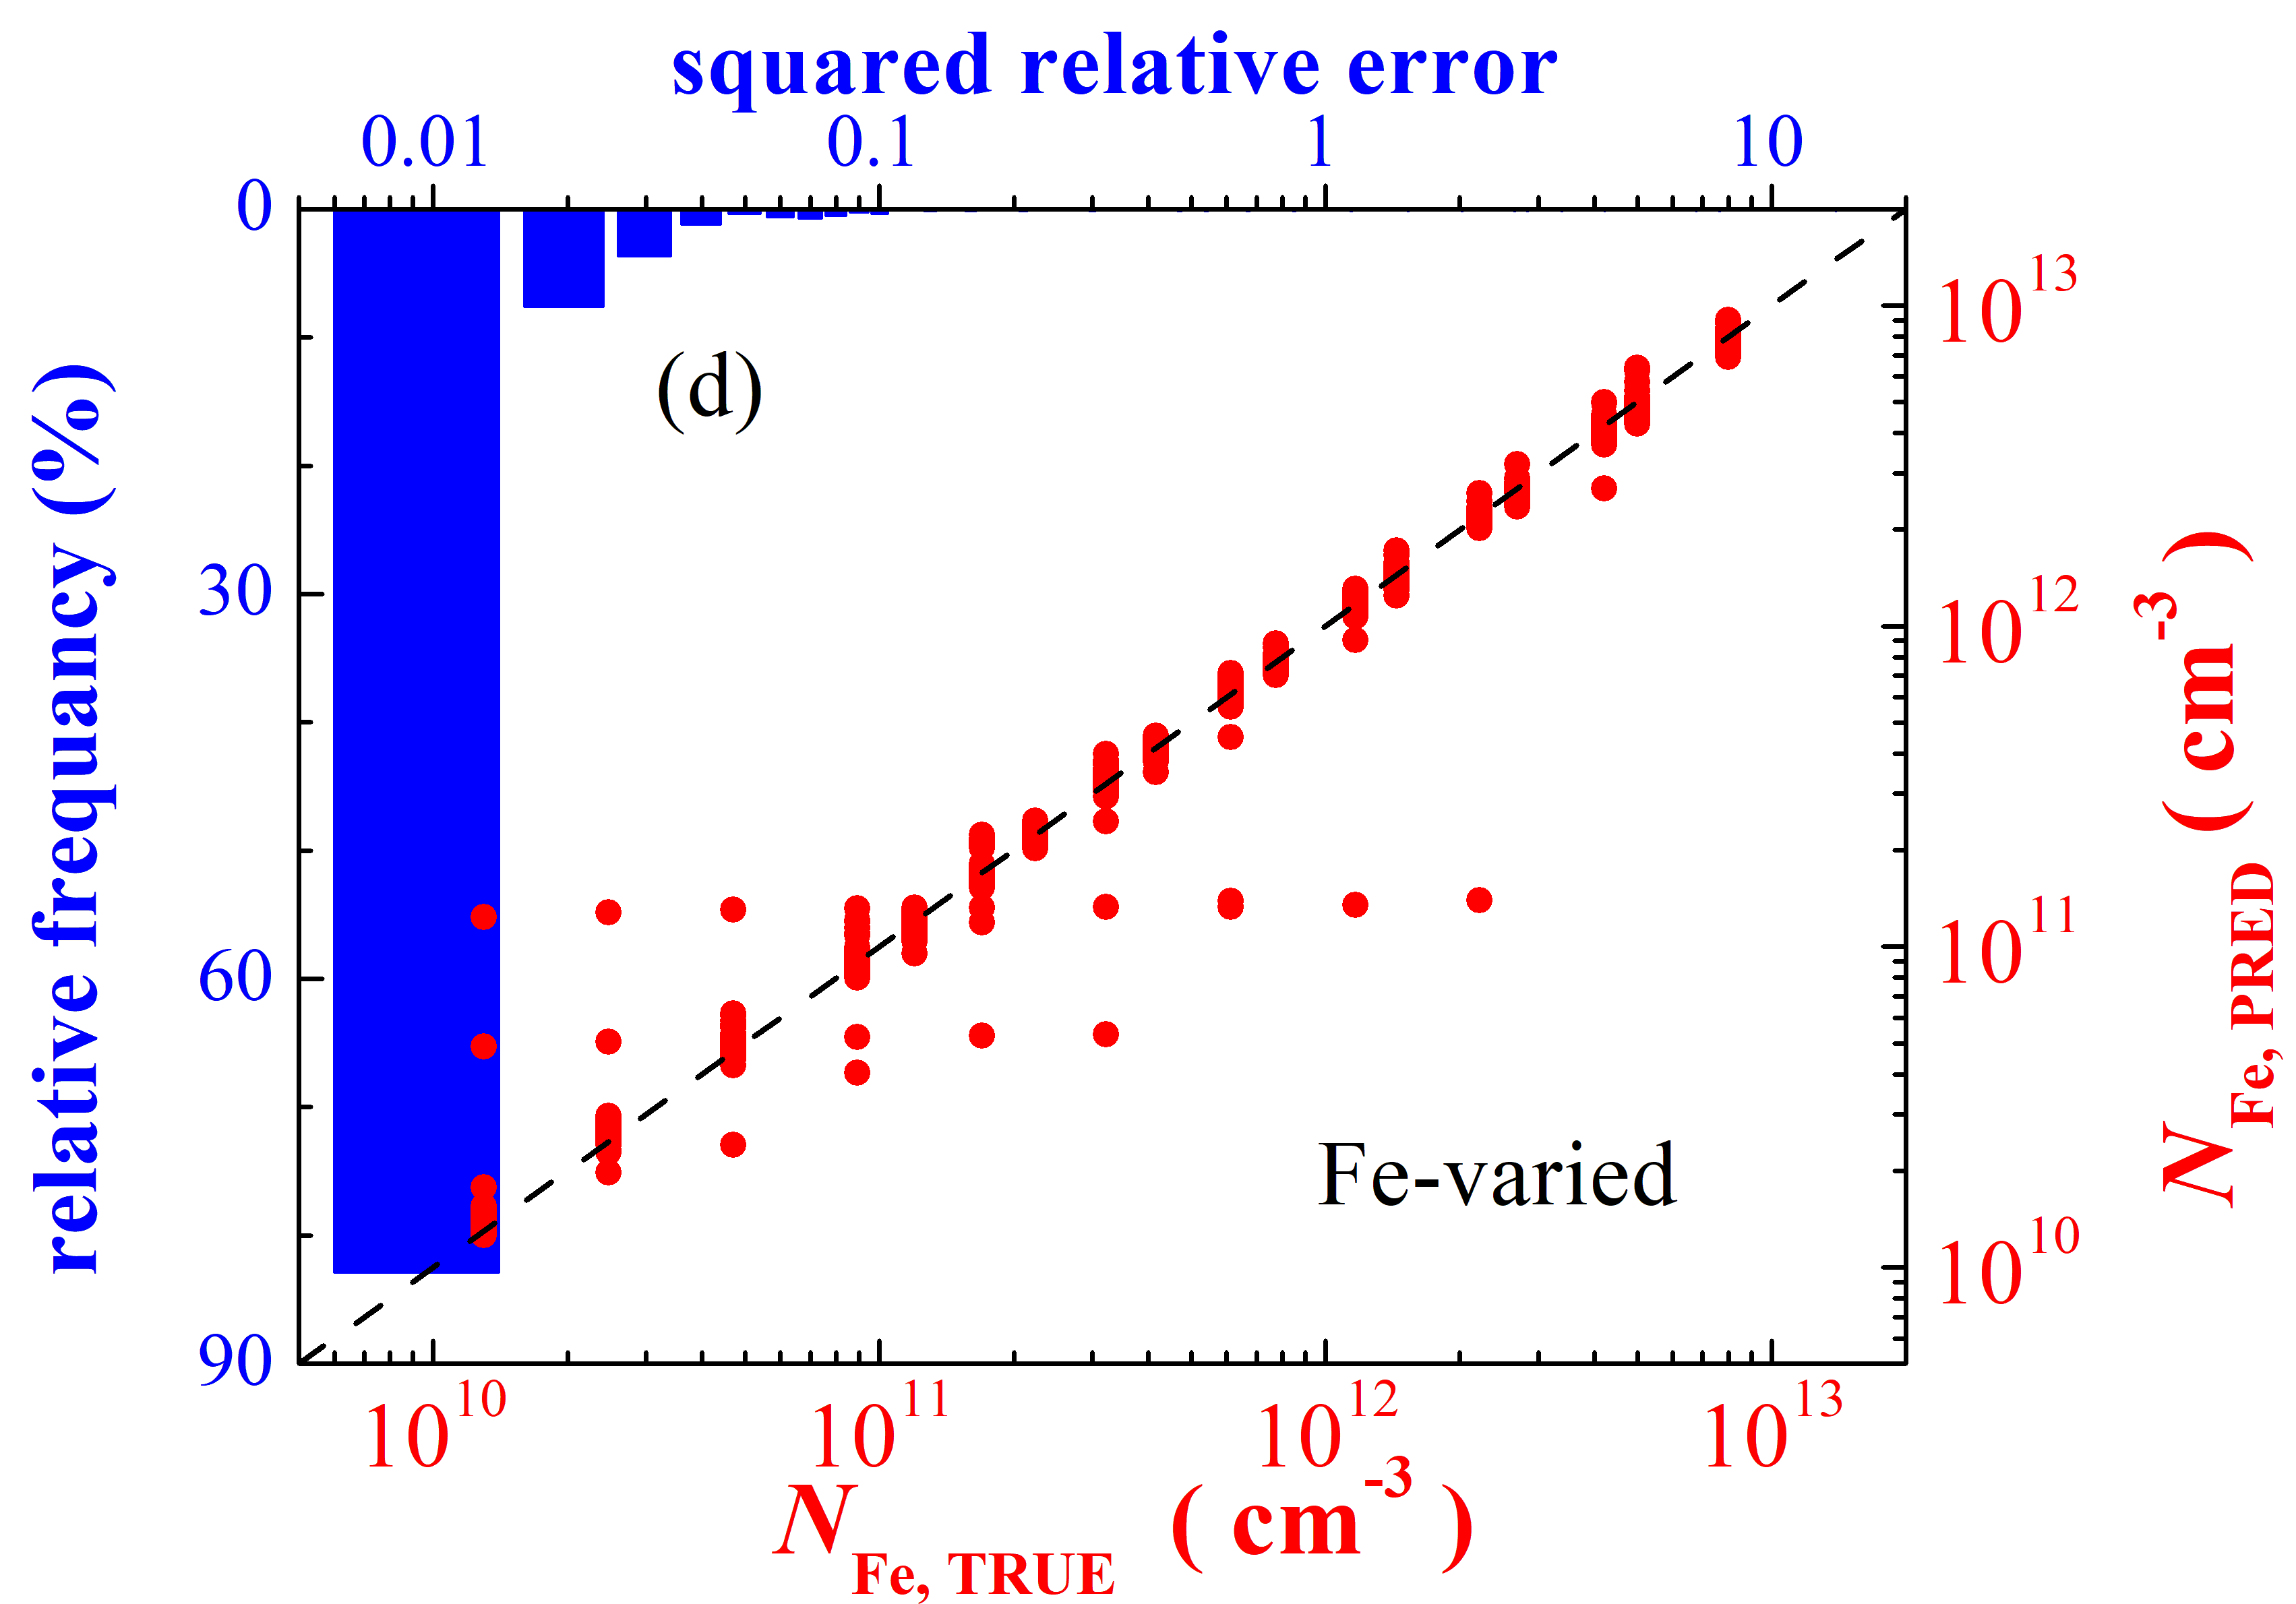
\includegraphics[width=0.32\textwidth]{F3d}
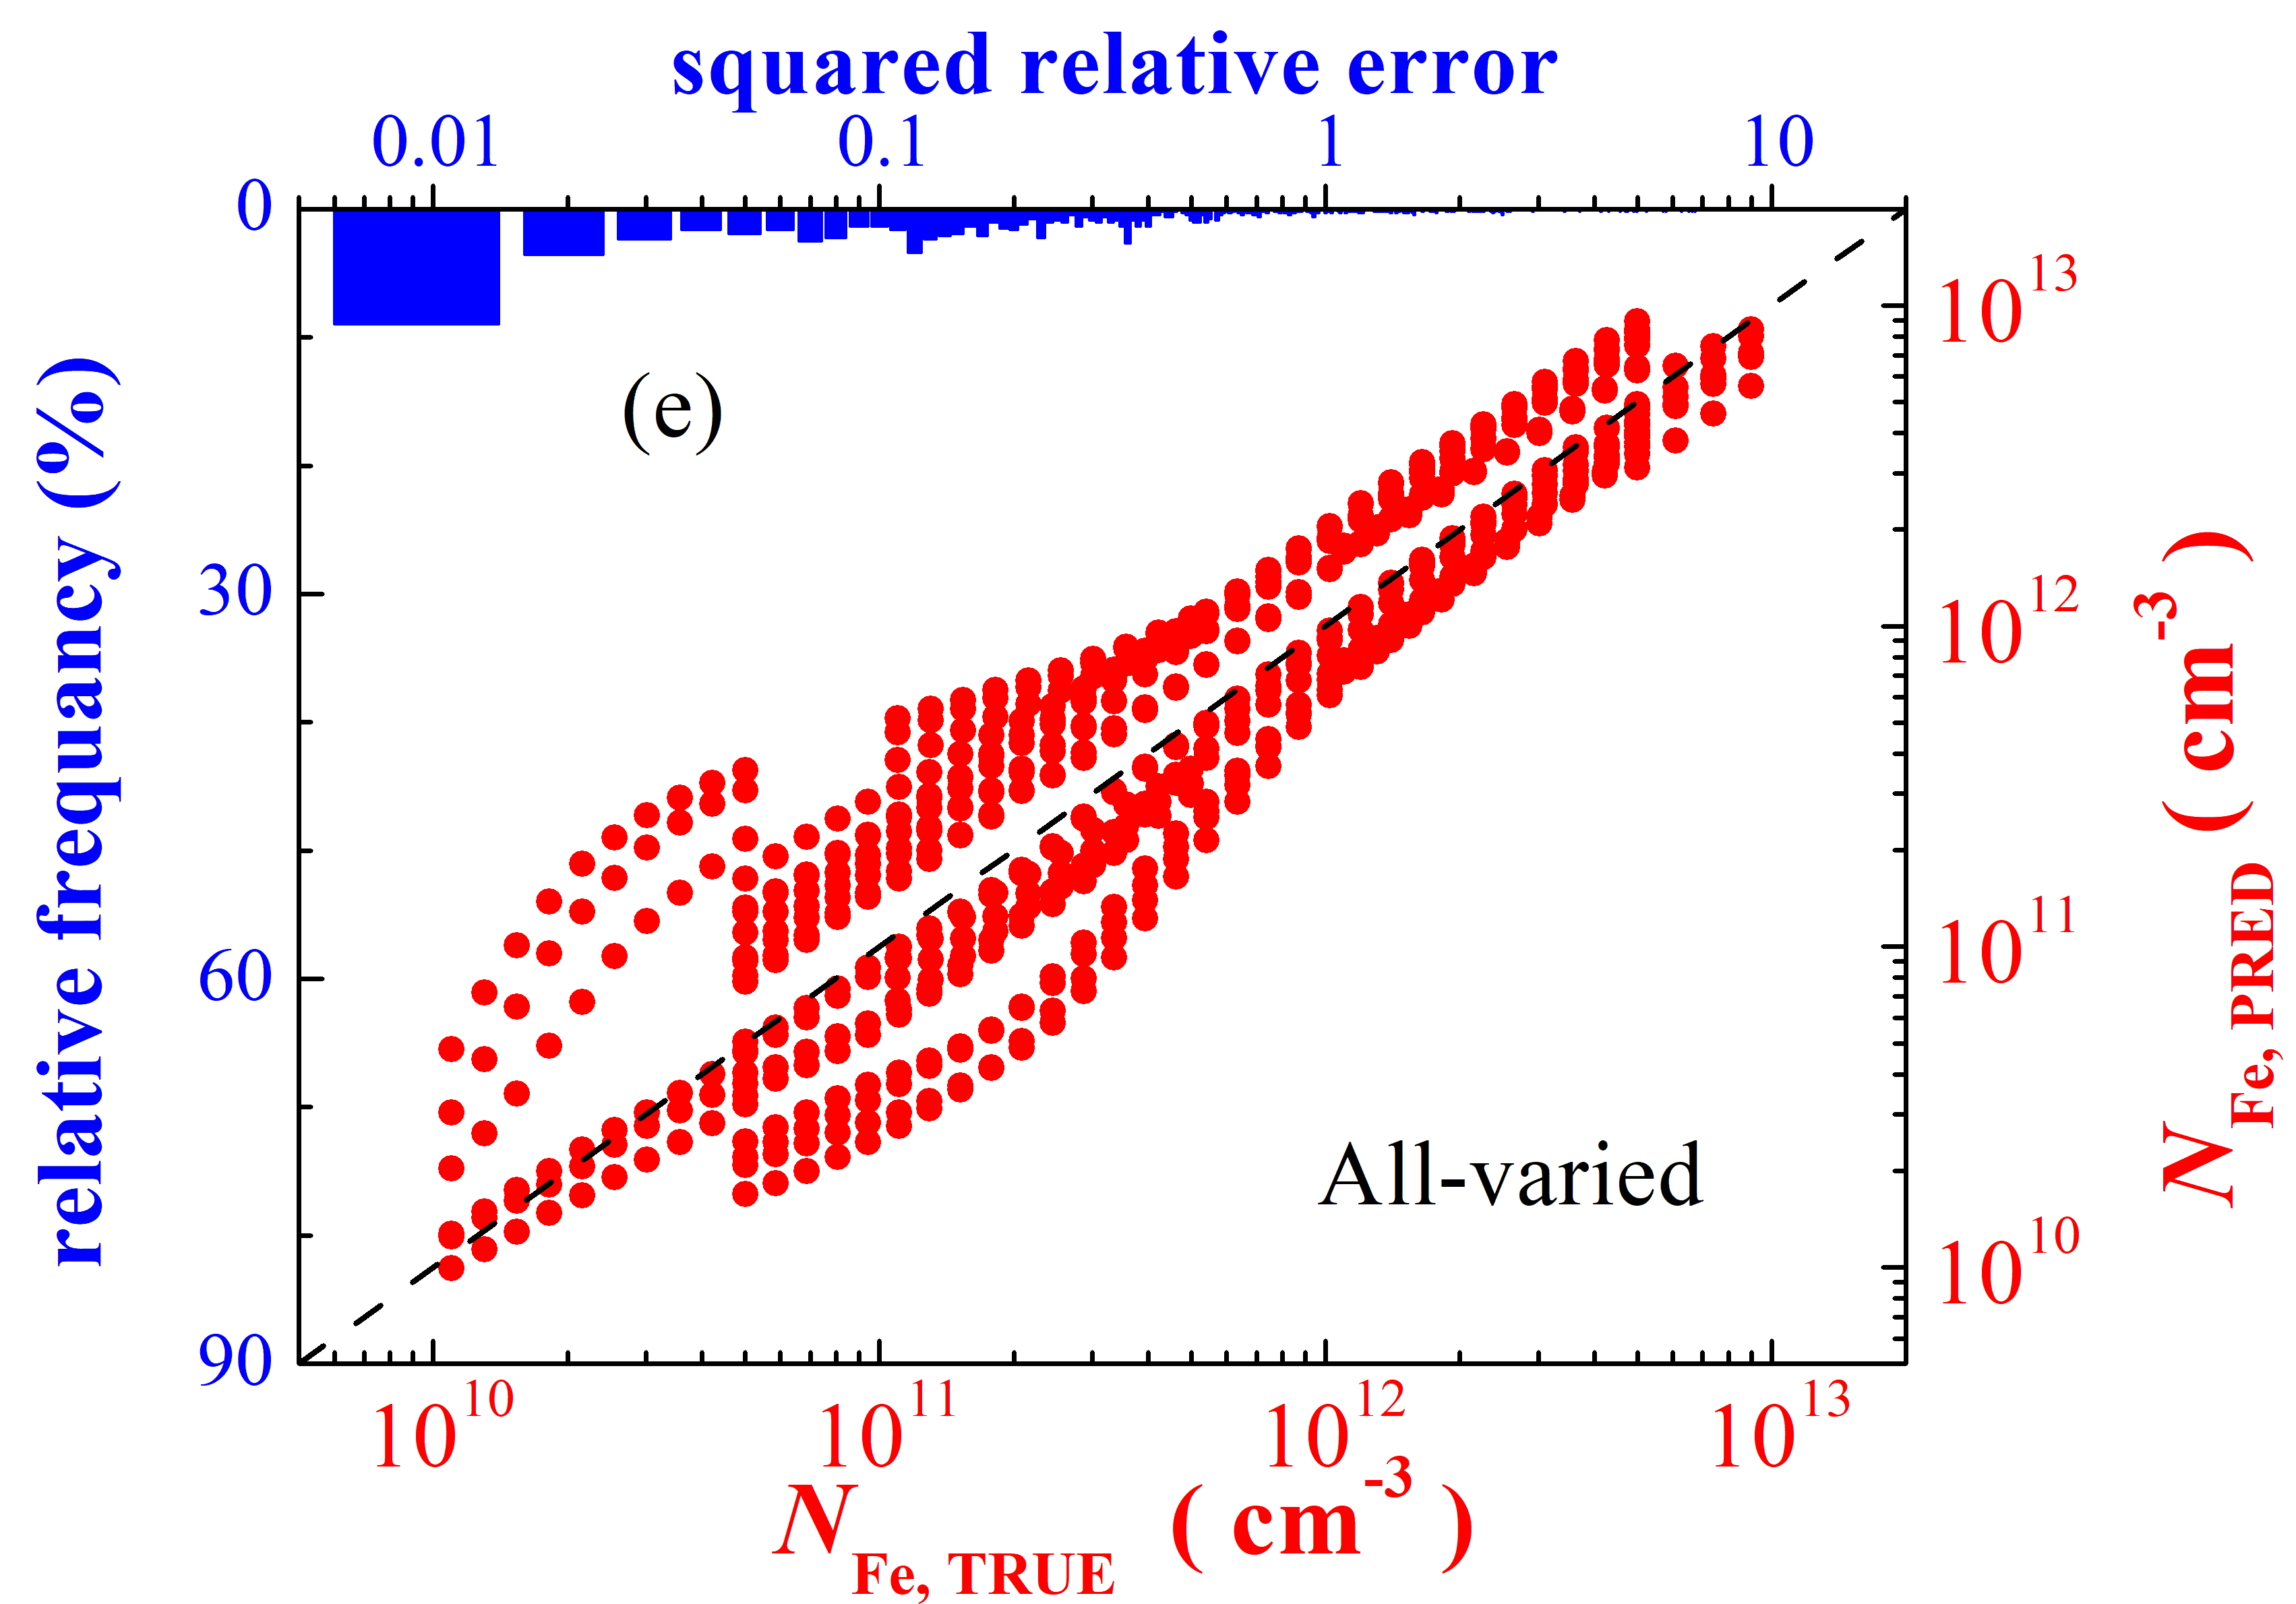
\includegraphics[width=0.32\textwidth]{F3e}
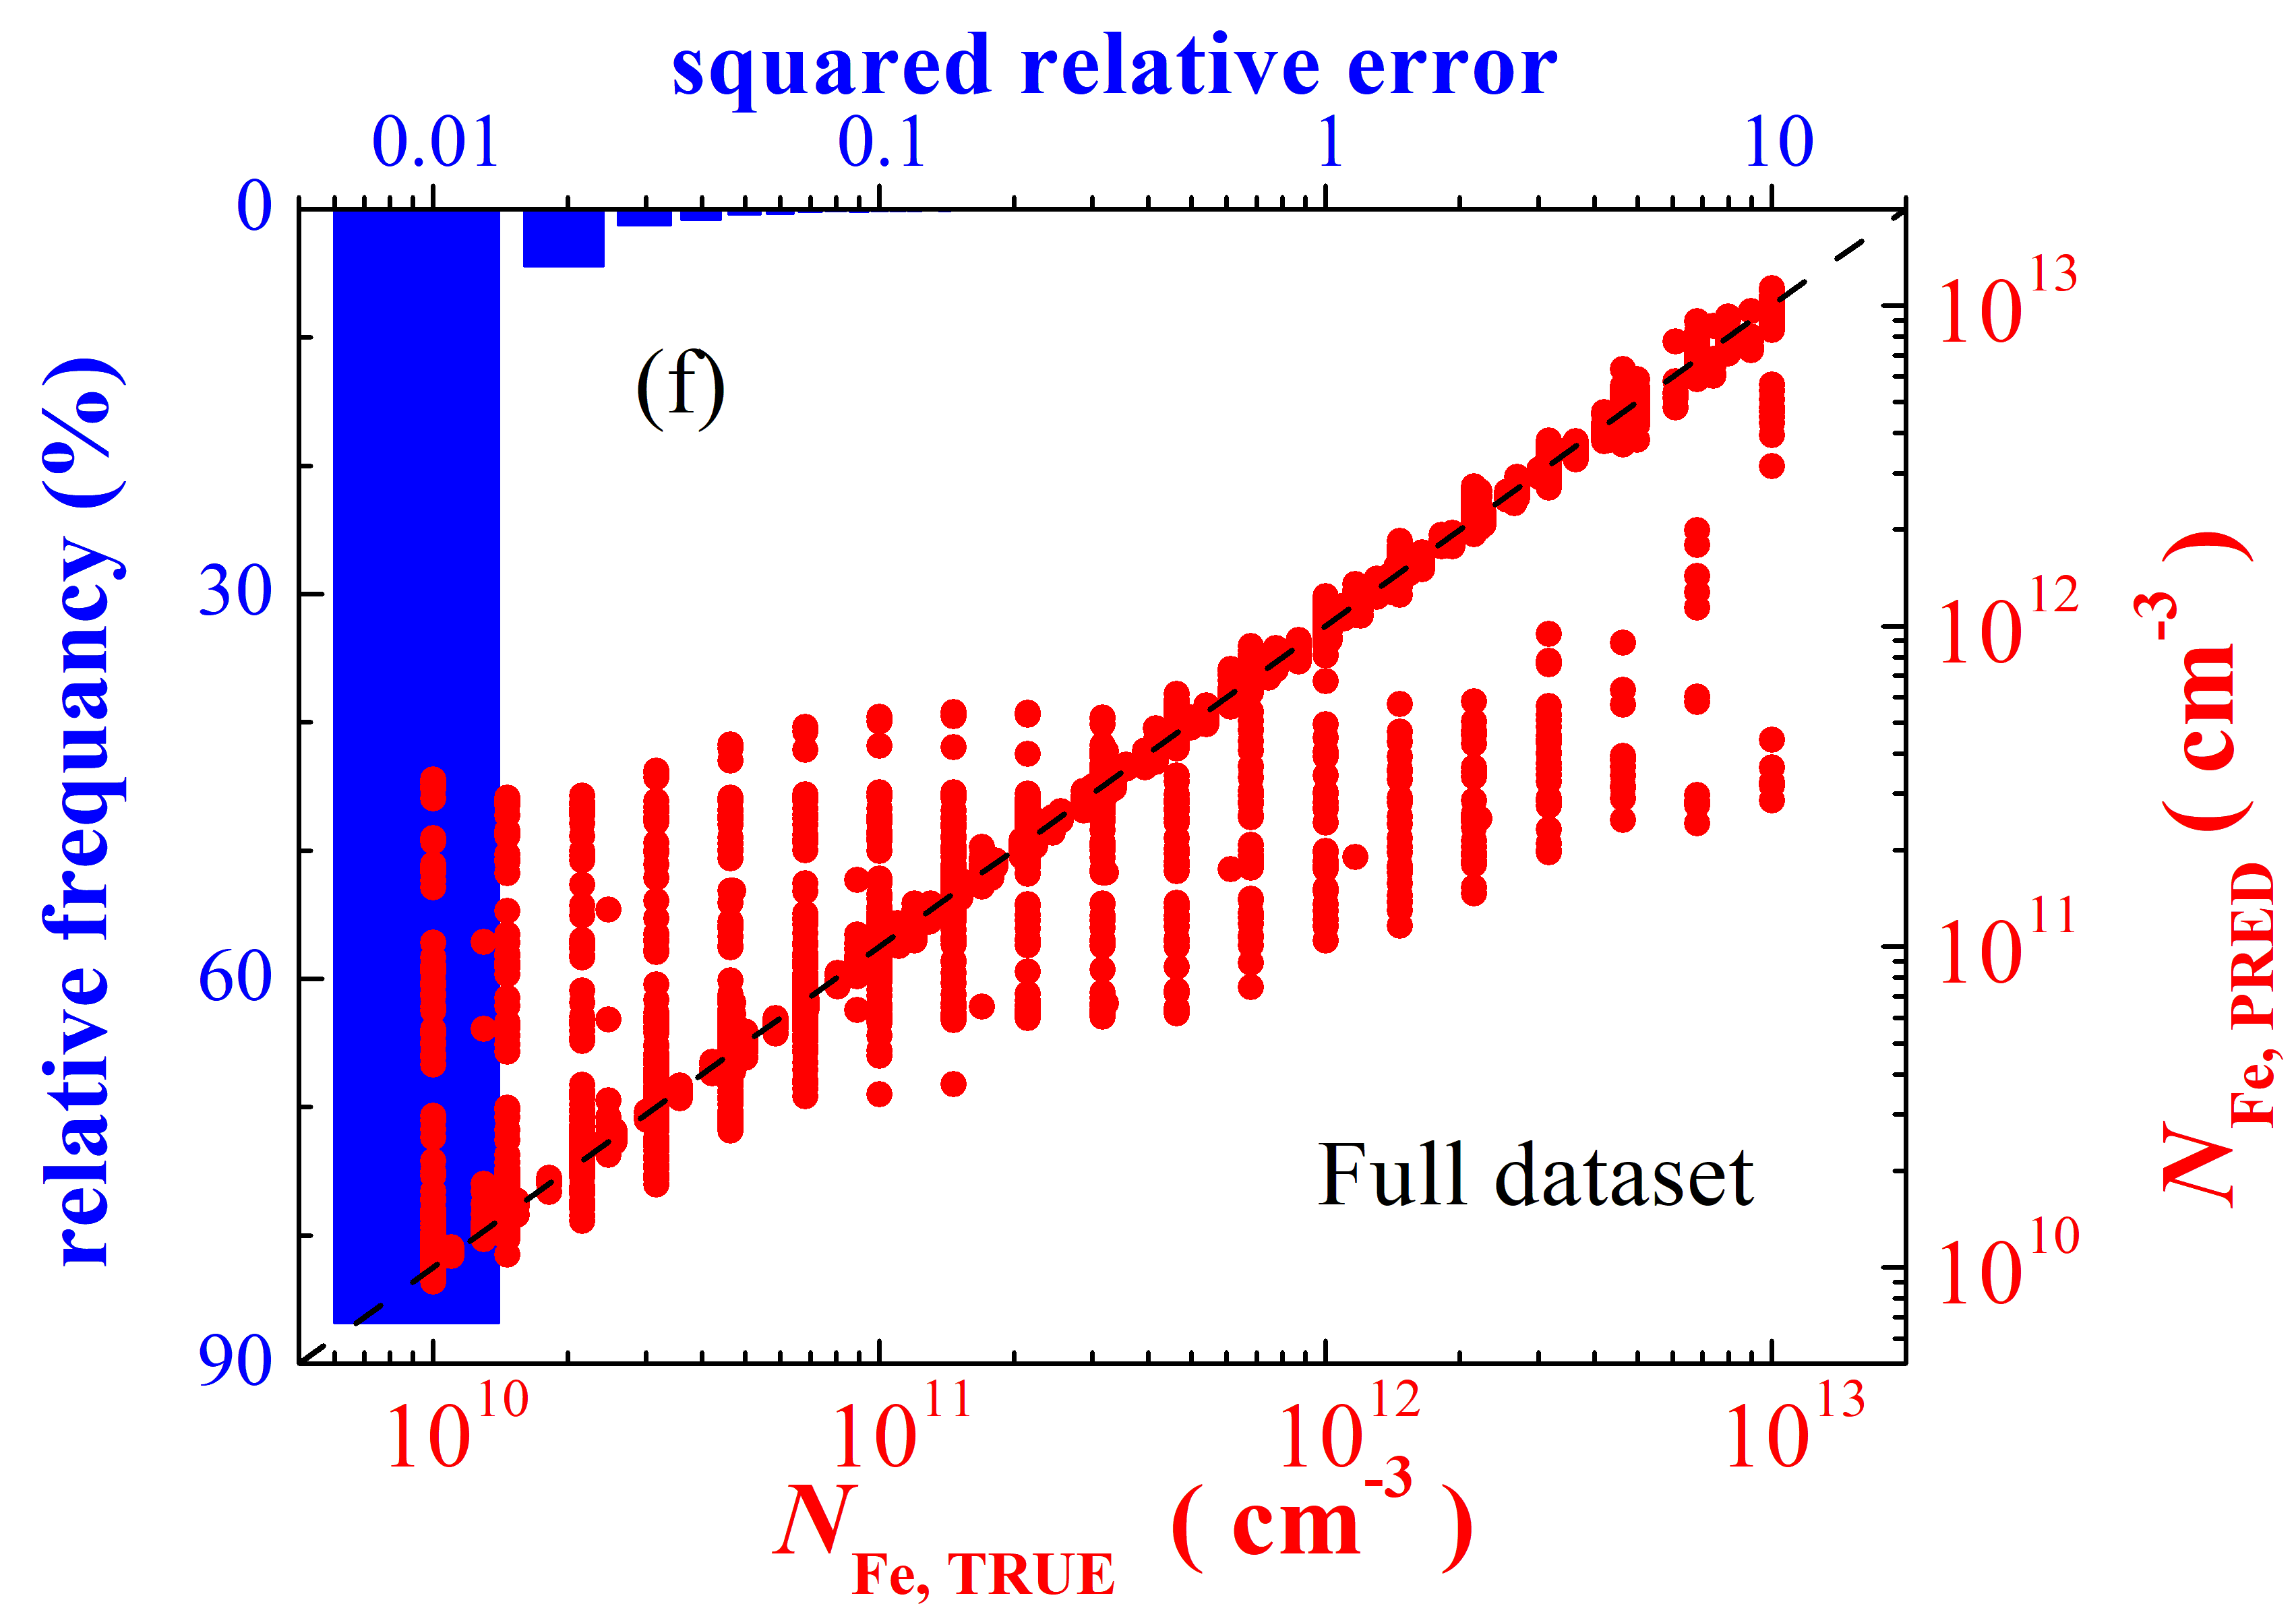
\includegraphics[width=0.32\textwidth]{F3f}
\caption{Iron concentrations are plotted against those generated by DNN$_\mathrm{FeFeB}$
on  T-varied (a),
d-varied (b),
B-varied (c),
Fe-varied (d),
All-varied (e),
and full (f) datasets (red points).
Bars represent histograms of squared relative error.
DNN was learned by training (a)--(e) or full (f) dataset.
The black dashed lines are the identify lines servings as the references.}
\label{fig_TrDNN1}
\end{figure}

We have also considered the DNN prediction error versus SC parameters  ---
see Figs.~\ref{fig_Temp}--~\ref{fig_Fe}.
The figures present data for training dataset; the results for test datasets are similar
(see Supplementary Material).
In particular, Fig.~\ref{fig_Temp}(a) shows a considerable increase in prediction error,
which is observed at $T>320$~K for DNN$_\mathrm{FeFeB}$.
As seen from Fig.~\ref{fig_Temp}(c), at $T=340$~K the maximum SRE is about 20 and
SRE below 0.01 is observed for 55\% of the samples
whereas these values are equal to 0.02 and 83\% at $T=290$~K
(Fig.~\ref{fig_Temp}(b)).
It has been shown previously \cite{OlikhJPS} that temperature rise causes the increase in
the intrinsic recombination contributions to the ideality factor.
As a result, the signature of Shockley-Read-Hall (SRH) recombination in $n$ value becomes less prominent
and DNN predictive ability decreases.

As shown in Fig.~\ref{fig_depth}, the SC base thickness practically does not influence the prediction error
(the mean value as well as relative frequency).
However, as seen from Fig.~\ref{fig_nValues}(c,d),
the ideality factor depends on base thickness at constant $N_\mathrm{Fe}$.
Therefore $d_p$ is a significant parameter for DNN training


\begin{figure}[tb]
\centering
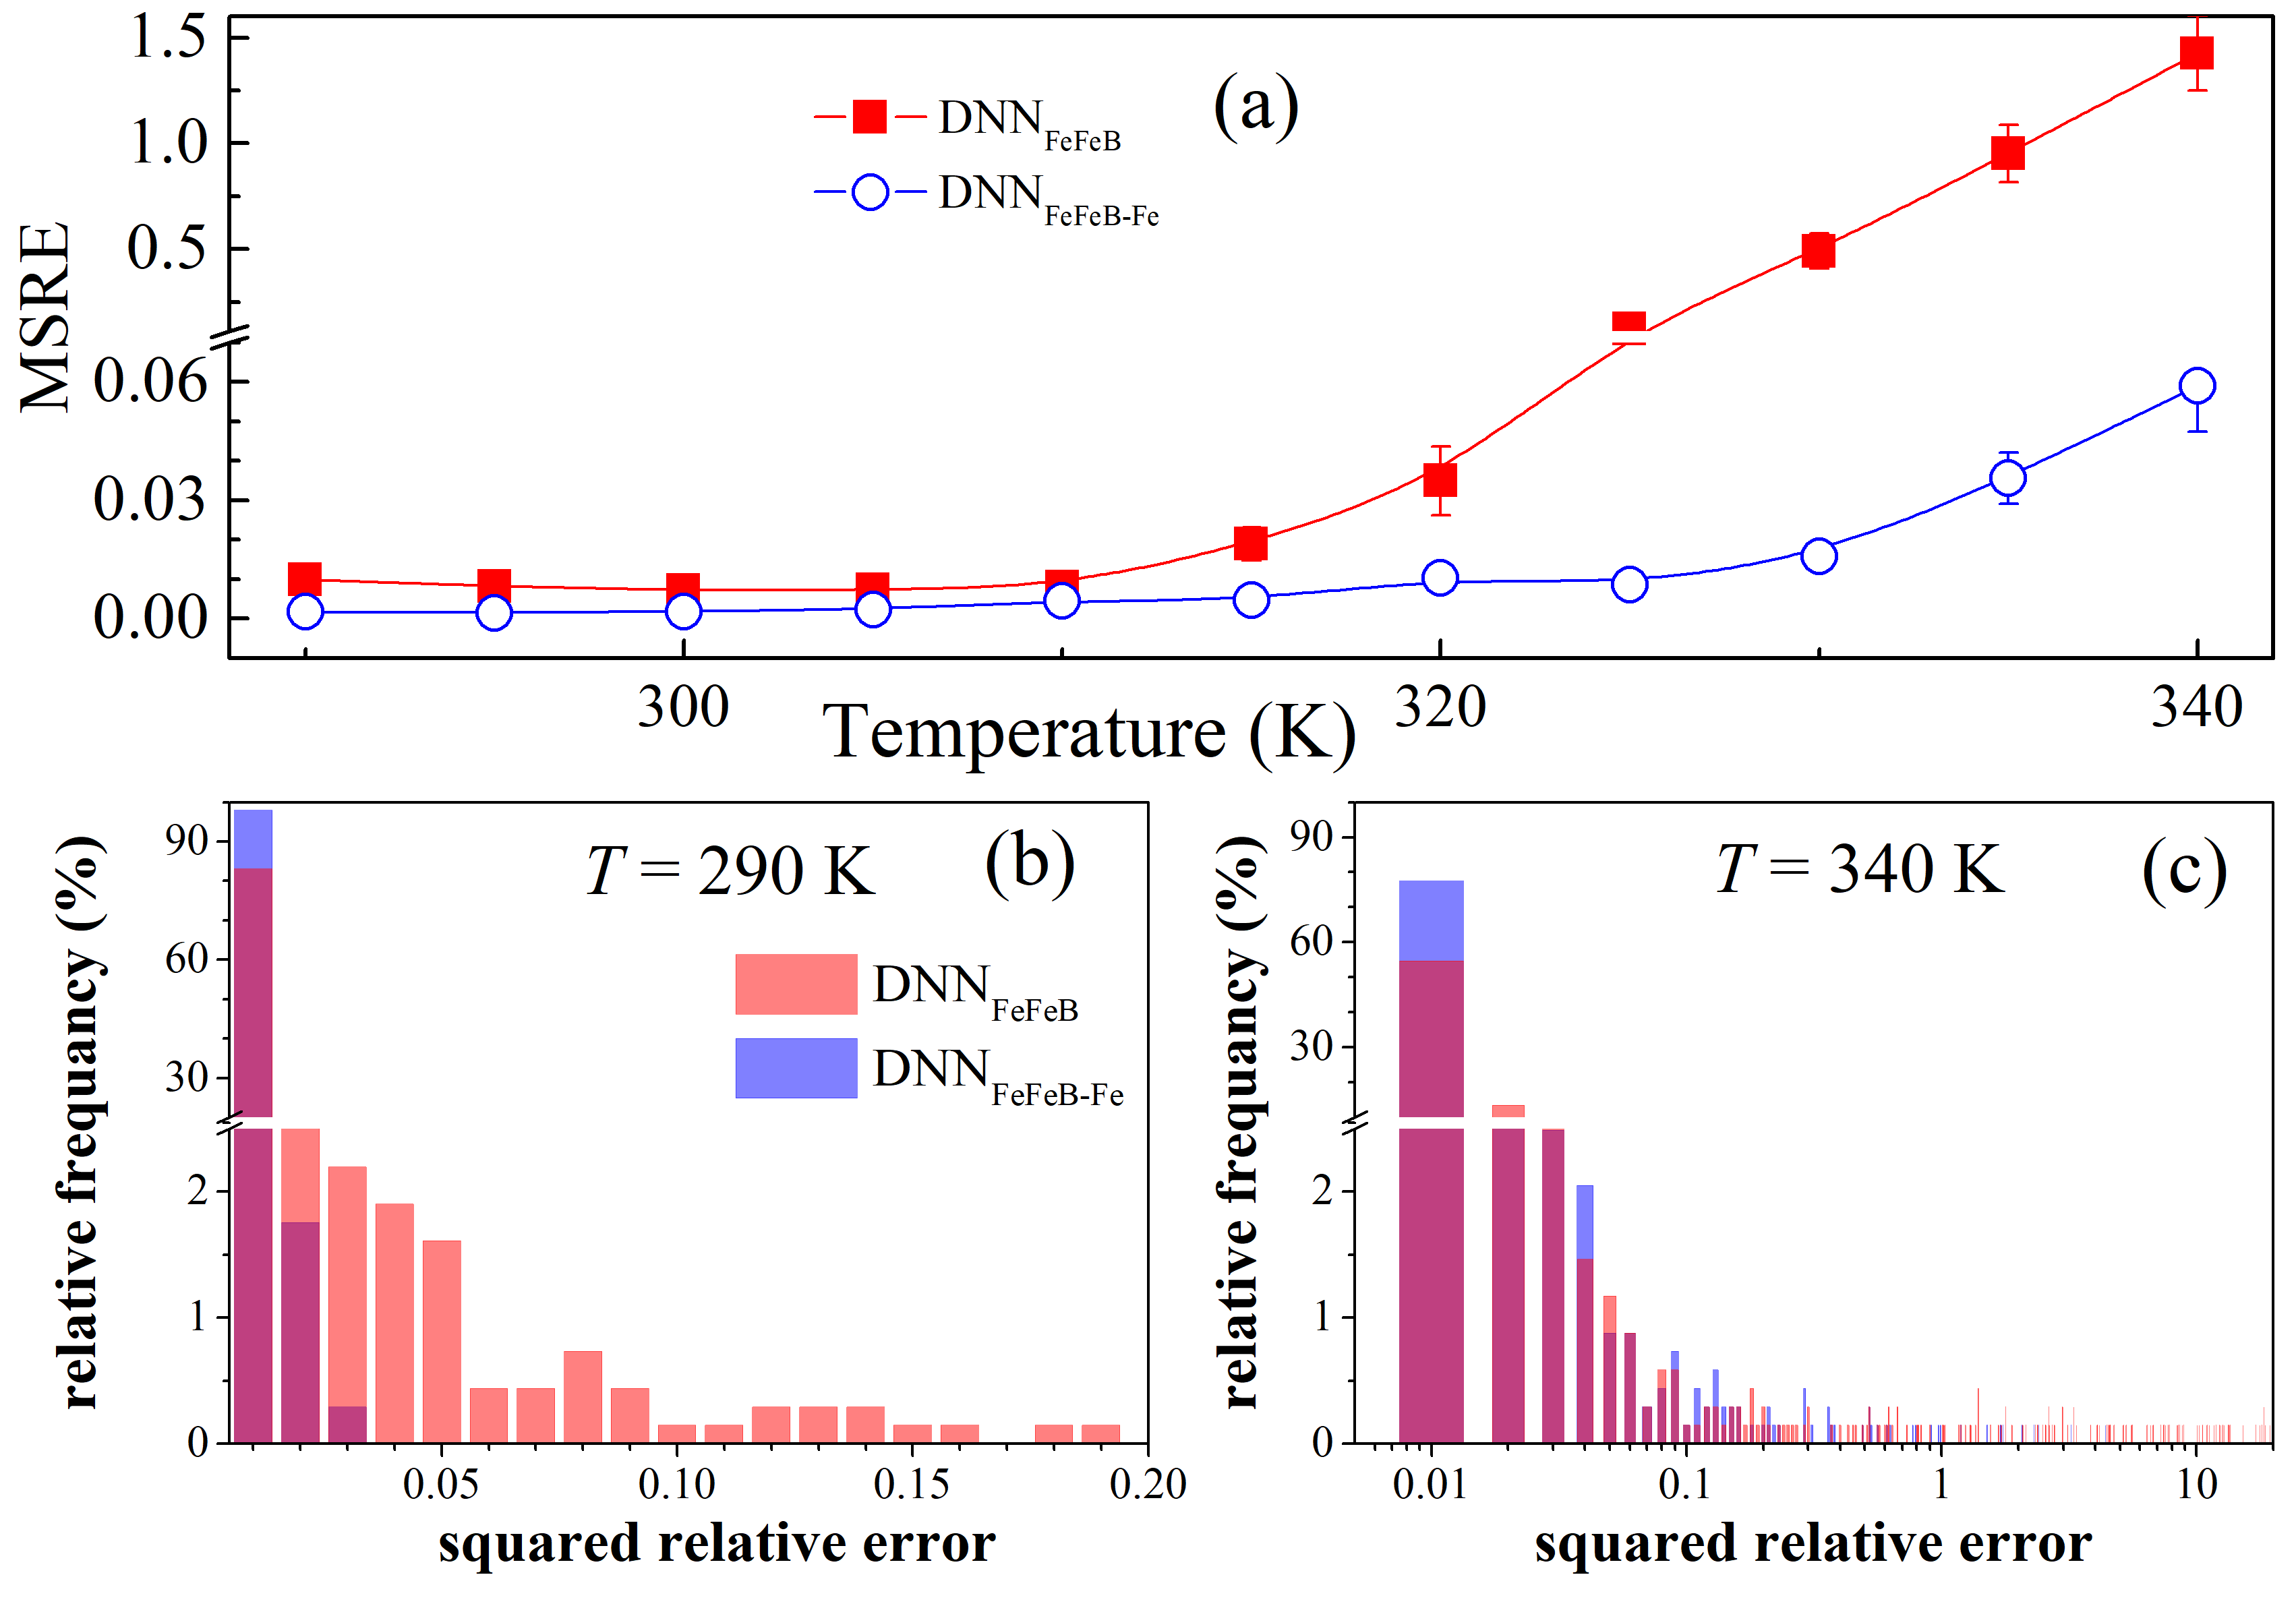
\includegraphics[width=0.48\textwidth]{F4} \hfill
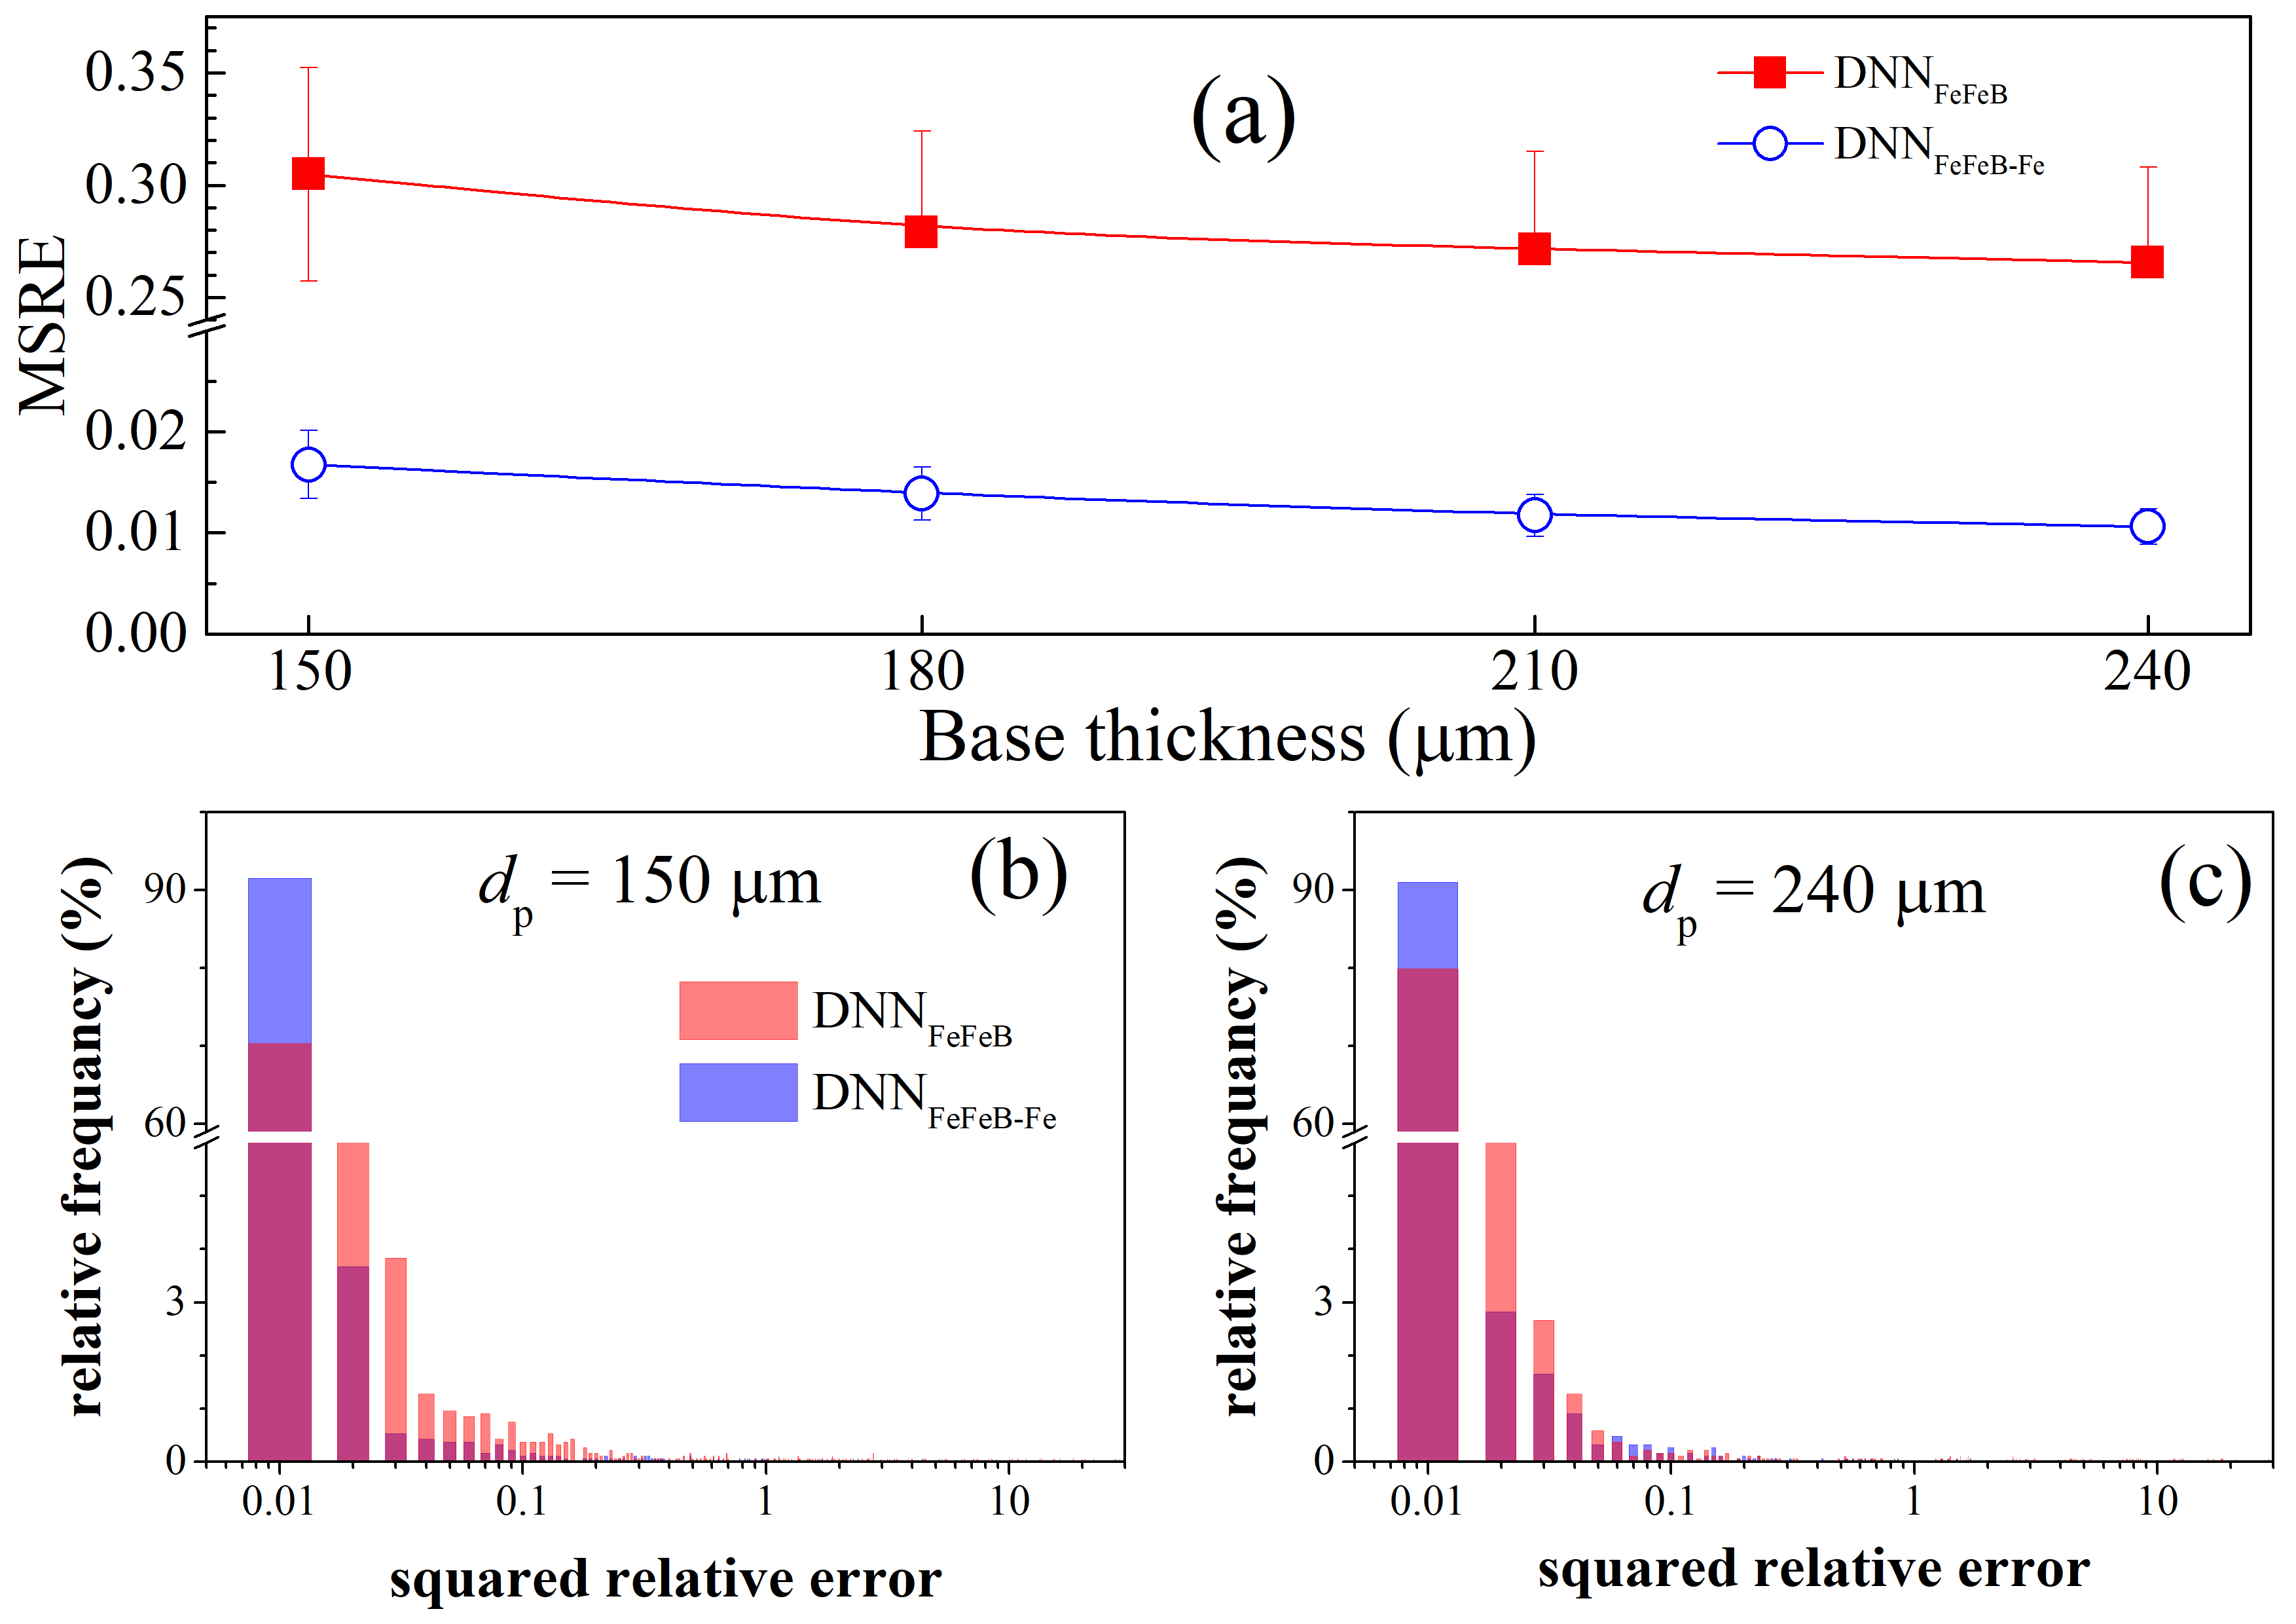
\includegraphics[width=0.48\textwidth]{F5} \\
\parbox[t]{0.48\textwidth}
{\caption{(a) Dependence of the MSRE (training dataset) on the temperature.
(b),(c) Histograms of squared relative error for $T=290$~K and $T=340$~K.
Red: DNN$_\mathrm{FeFeB}$; blue: DNN$_\mathrm{FeFeB-Fe}$.
}
\label{fig_Temp}} \hfill
\parbox[t]{0.48\textwidth}{\caption{(a) Dependence of the MSRE (training dataset) on the base thickness.
(b),(c) Histograms of squared relative error for $d_p=150$~$\mu$m and $d_p=240$~$\mu$m.
Red: DNN$_\mathrm{FeFeB}$; blue: DNN$_\mathrm{FeFeB-Fe}$.}
\label{fig_depth}}
\end{figure}

The predictive error increases sharply as the doping level decreases --- see Fig.~\ref{fig_B}(a).
In particular,  the maximum SRE is about 0.05 for $N_\mathrm{B}=10^{17}$~cm$^{-3}$ (Fig.~\ref{fig_B}(c))
whereas SRE below 0.05 is only for 56\% of samples with $N_\mathrm{B}=10^{15}$~cm$^{-3}$ (Fig.~\ref{fig_B}(b)).
The occupation of holes in Fe-related level determines SRH recombination efficiency.
According to the Fermi-Dirac statistics,
the probability of hole occupation in a non-degenerate $p$-type semiconductor with full acceptor depletion can be expressed as
\begin{equation}
\label{eqfp}
 f_p=\frac{1}{1+\frac{N_V}{N_\mathrm{B}}\exp\left(\frac{E_V-E_{\mathrm{Fe}_i}}{kT}\right)}\,.
\end{equation}
If $N_\mathrm{B}$ decreases, the level is filled with the electron,
the SRH recombination stops
and the ideality factor value sharply decreases  --- Fig.~\ref{fig_nValues}(a,b).
Moreover, in case of low doping,   impurities have only a weak influence
on the ideality factor, and therefore the increase of MSRE is observed.
And finally, we believe that the additional factor causing the error to increase
at high temperatures is the level filling.


\begin{figure}[tb]
\centering
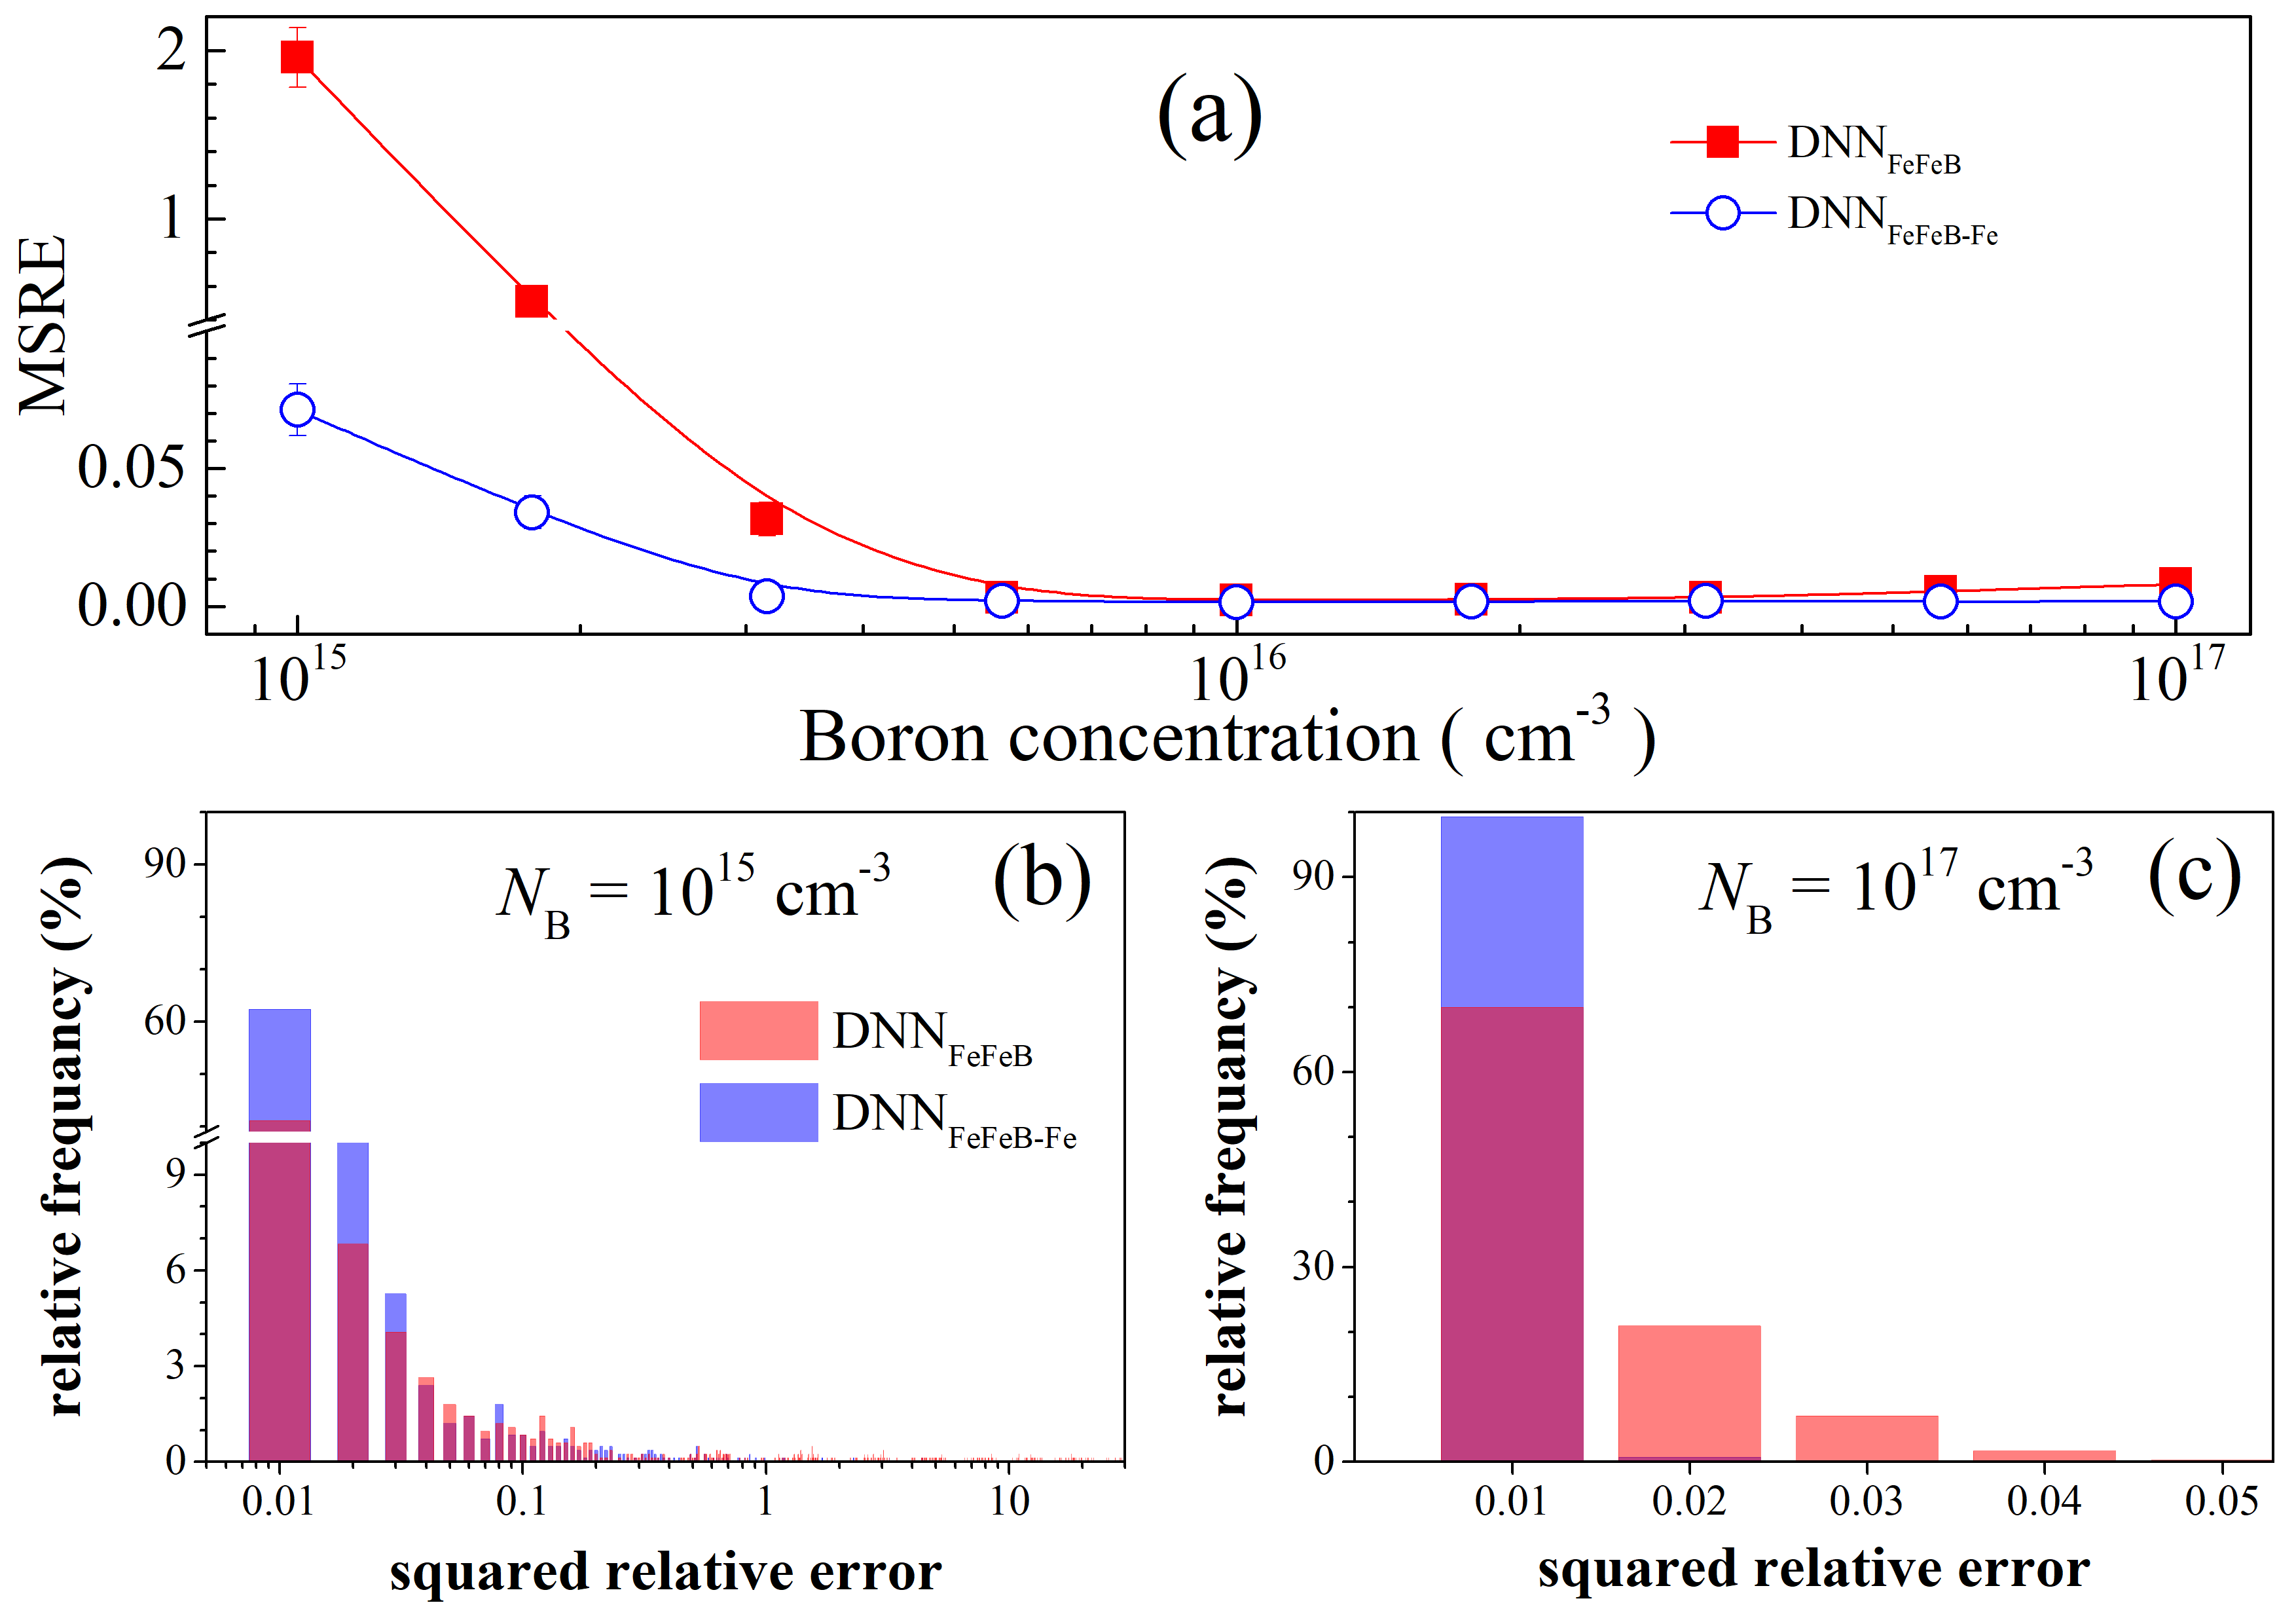
\includegraphics[width=0.48\textwidth]{F6} \hfill
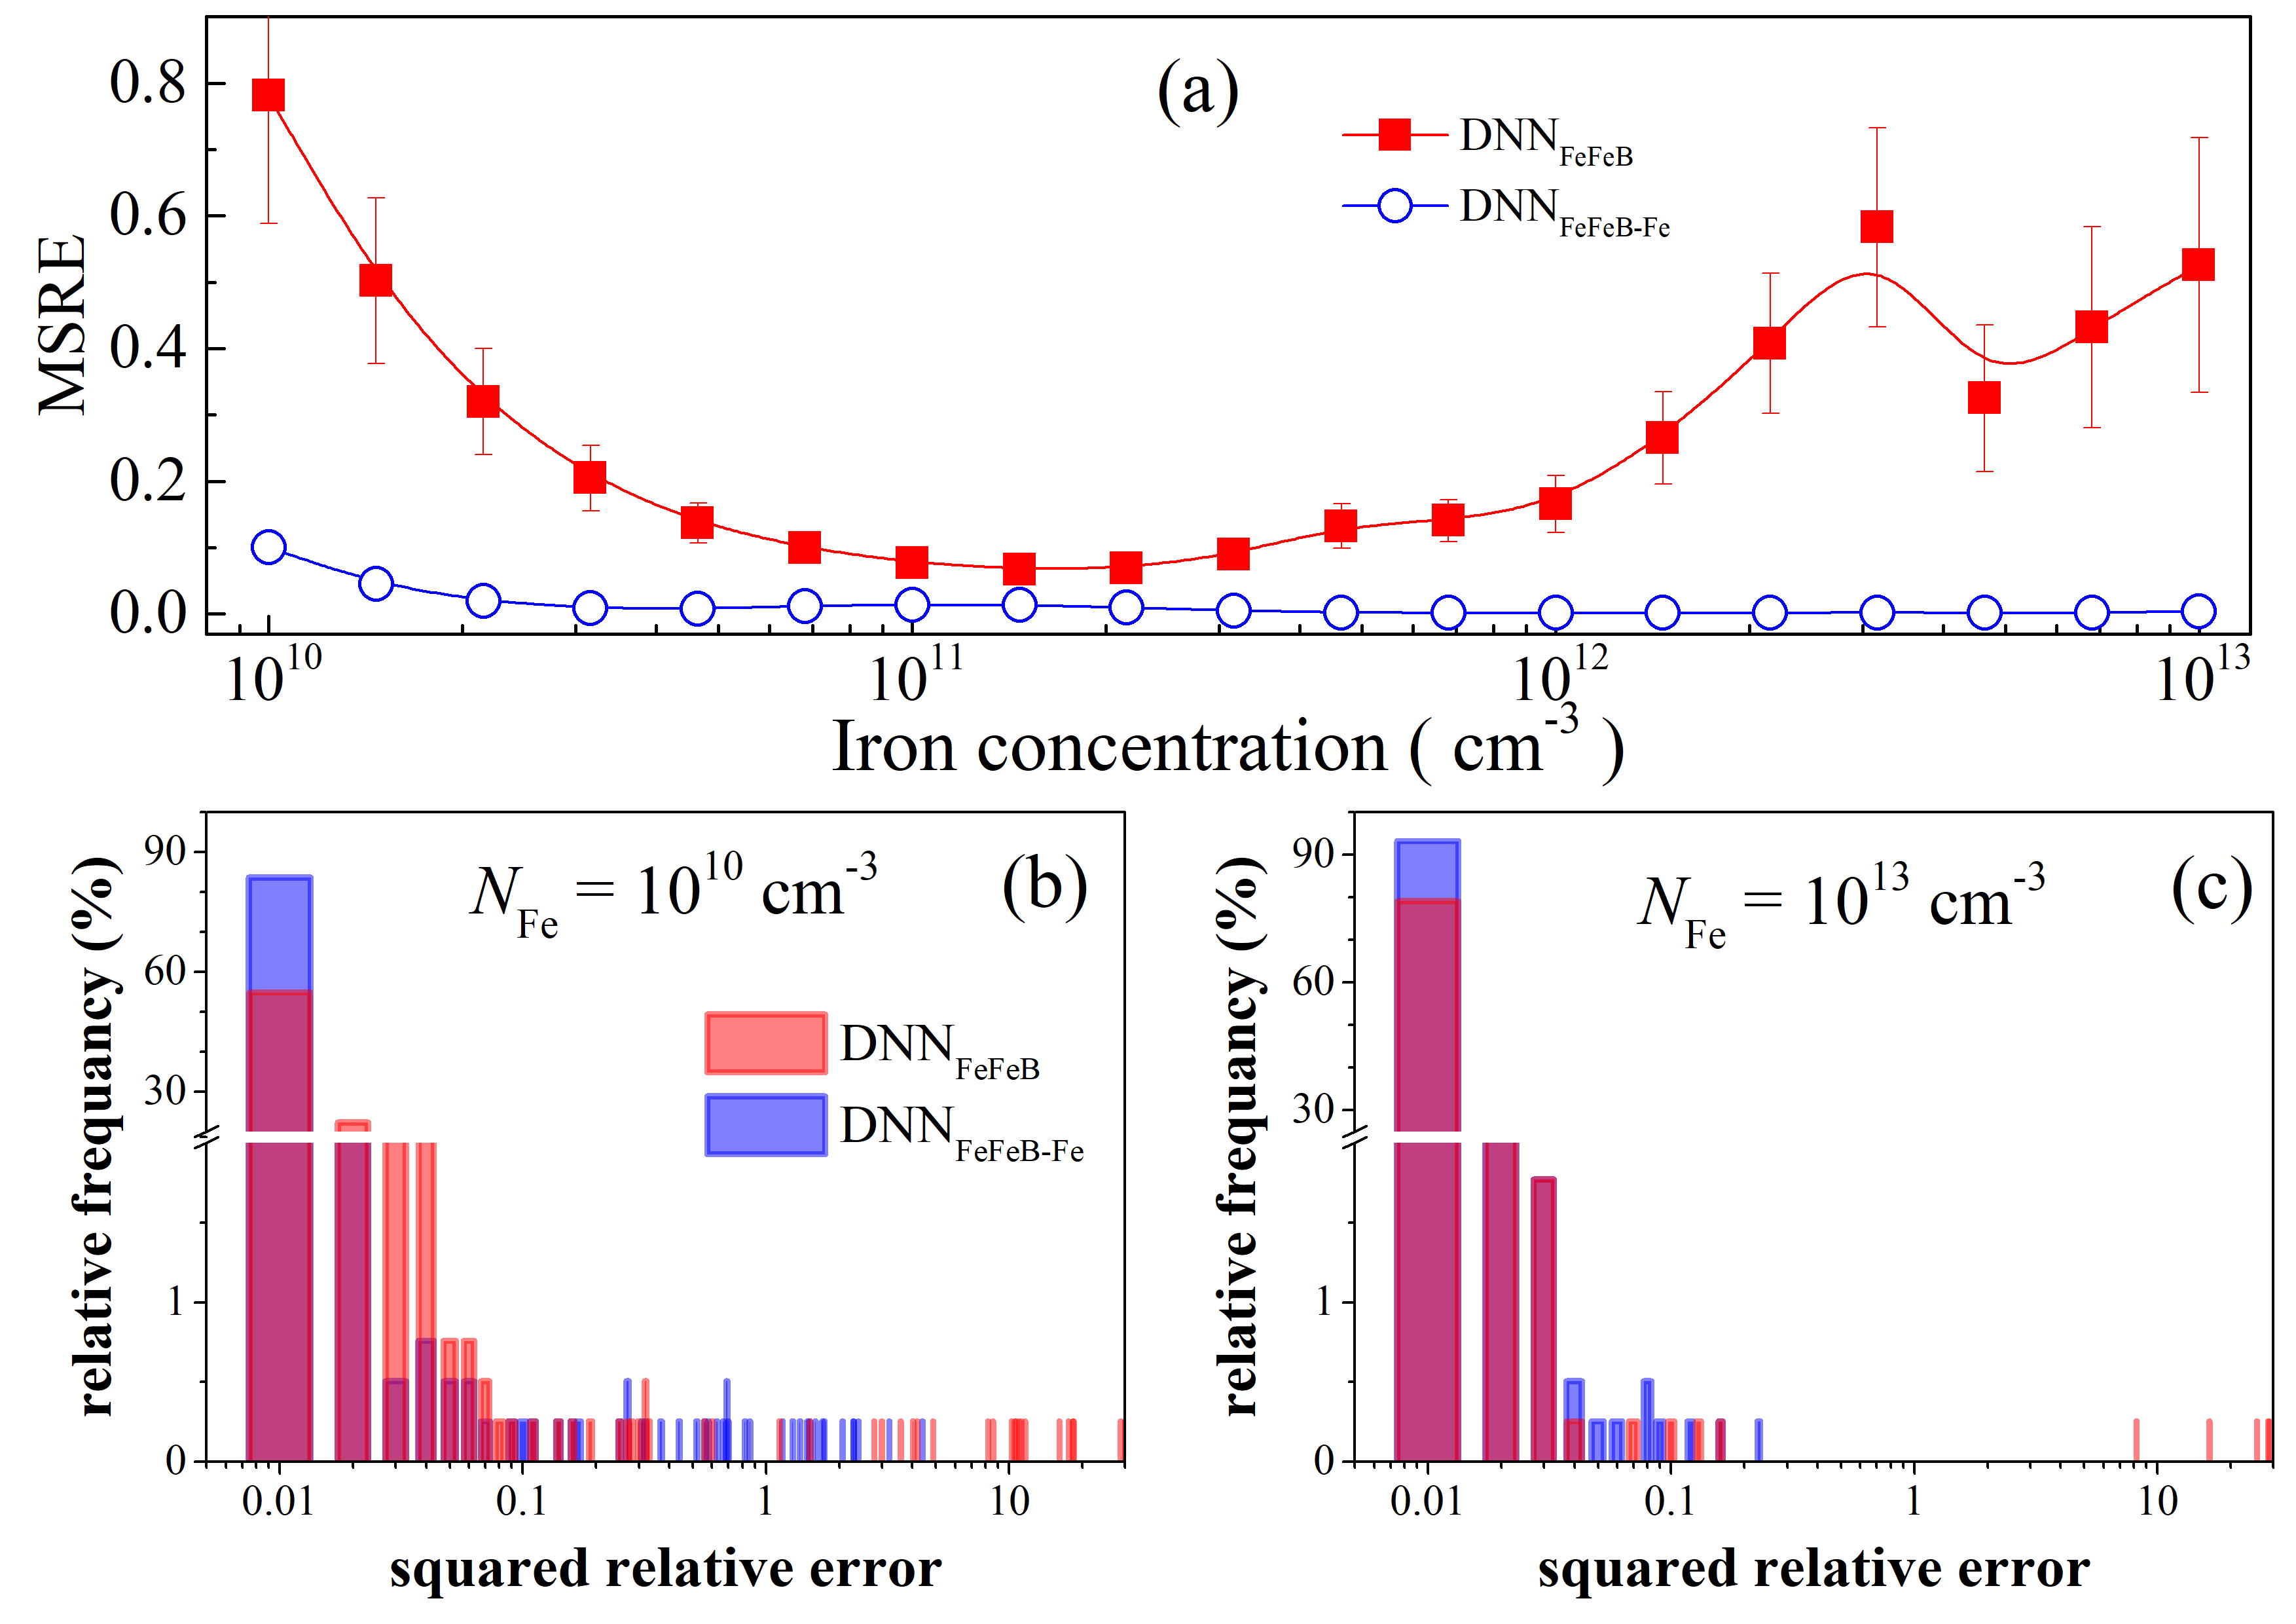
\includegraphics[width=0.48\textwidth]{F7} \\
\parbox[t]{0.48\textwidth}
{\caption{(a) Dependence of the MSRE (training dataset) on the boron concentration.
(b),(c) Histograms of squared  relative error for $N_\mathrm{B}=10^{15}$~cm$^{-3}$ and $N_\mathrm{B}=10^{17}$~cm$^{-3}$.
Red: DNN$_\mathrm{FeFeB}$; blue: DNN$_\mathrm{FeFeB-Fe}$.
}
\label{fig_B}} \hfill
\parbox[t]{0.48\textwidth}{\caption{(a) Dependence of the MSRE (training dataset) on the iron concentration.
(b),(c) Histograms of squared  relative error for $N_\mathrm{Fe}=10^{10}$~cm$^{-3}$ and $N_\mathrm{Fe}=10^{13}$~cm$^{-3}$.
Red: DNN$_\mathrm{FeFeB}$; blue: DNN$_\mathrm{FeFeB-Fe}$.}
\label{fig_Fe}}
\end{figure}

Fig.~\ref{fig_Fe}(a) shows that MSRE increases at both low and high iron concentrations.
The first $N_\mathrm{Fe}$ area of poor DNN accuracy is entirely predictable,
the second one seems to be rather surprising.
But according to Fig~\ref{fig_Fe}(c), the MSRE increase is most likely to be due to the fact
that only a few samples are predicted with a great SRE
at $N_\mathrm{Fe}=10^{13}$~cm$^{-3}$
whereas SRE increases more systematically when $N_\mathrm{Fe}=10^{13}$~cm$^{-3}$ --- Fig~\ref{fig_Fe}(b).

The ideality factor value for the case when only interstitial iron ($n_\mathrm{Fe}$)
is available gives extra information about the defects in comparison with $n_\mathrm{Fe-FeB}$.
It is not surprising that DNN$_\mathrm{FeFeB-Fe}$ has better operating parameters compared to
DNN$_\mathrm{FeFeB}$ --- see Table~\ref{table_CV}, Table~\ref{table_MSRE}, Fig.~\ref{fig_TrDNN2}.
The predictions improve:
MSRE decreases,
there is no huge difference between the values of $N_\mathrm{Fe,TRUE}$ and $N_\mathrm{Fe,PRED}$,
the range of SRE becomes  narrow
(Figs.~\ref{fig_Temp}-\ref{fig_TrDNN2}).
As shown in Fig.~\ref{fig_TrDNN2}, the maximum SRE does not exceed one even in the case of All-varied dataset,
and SRE is below 0.02 for 93\%, 92\%, 73\%, and 97\% of the samples in T-varied, d-varied, B-varied, and Fe-varied datasets respectively.
It should be noted that  for Fe-varied datasets both $R^2$ and  $R$  are 0.999.


\begin{figure}[bt]
\centering
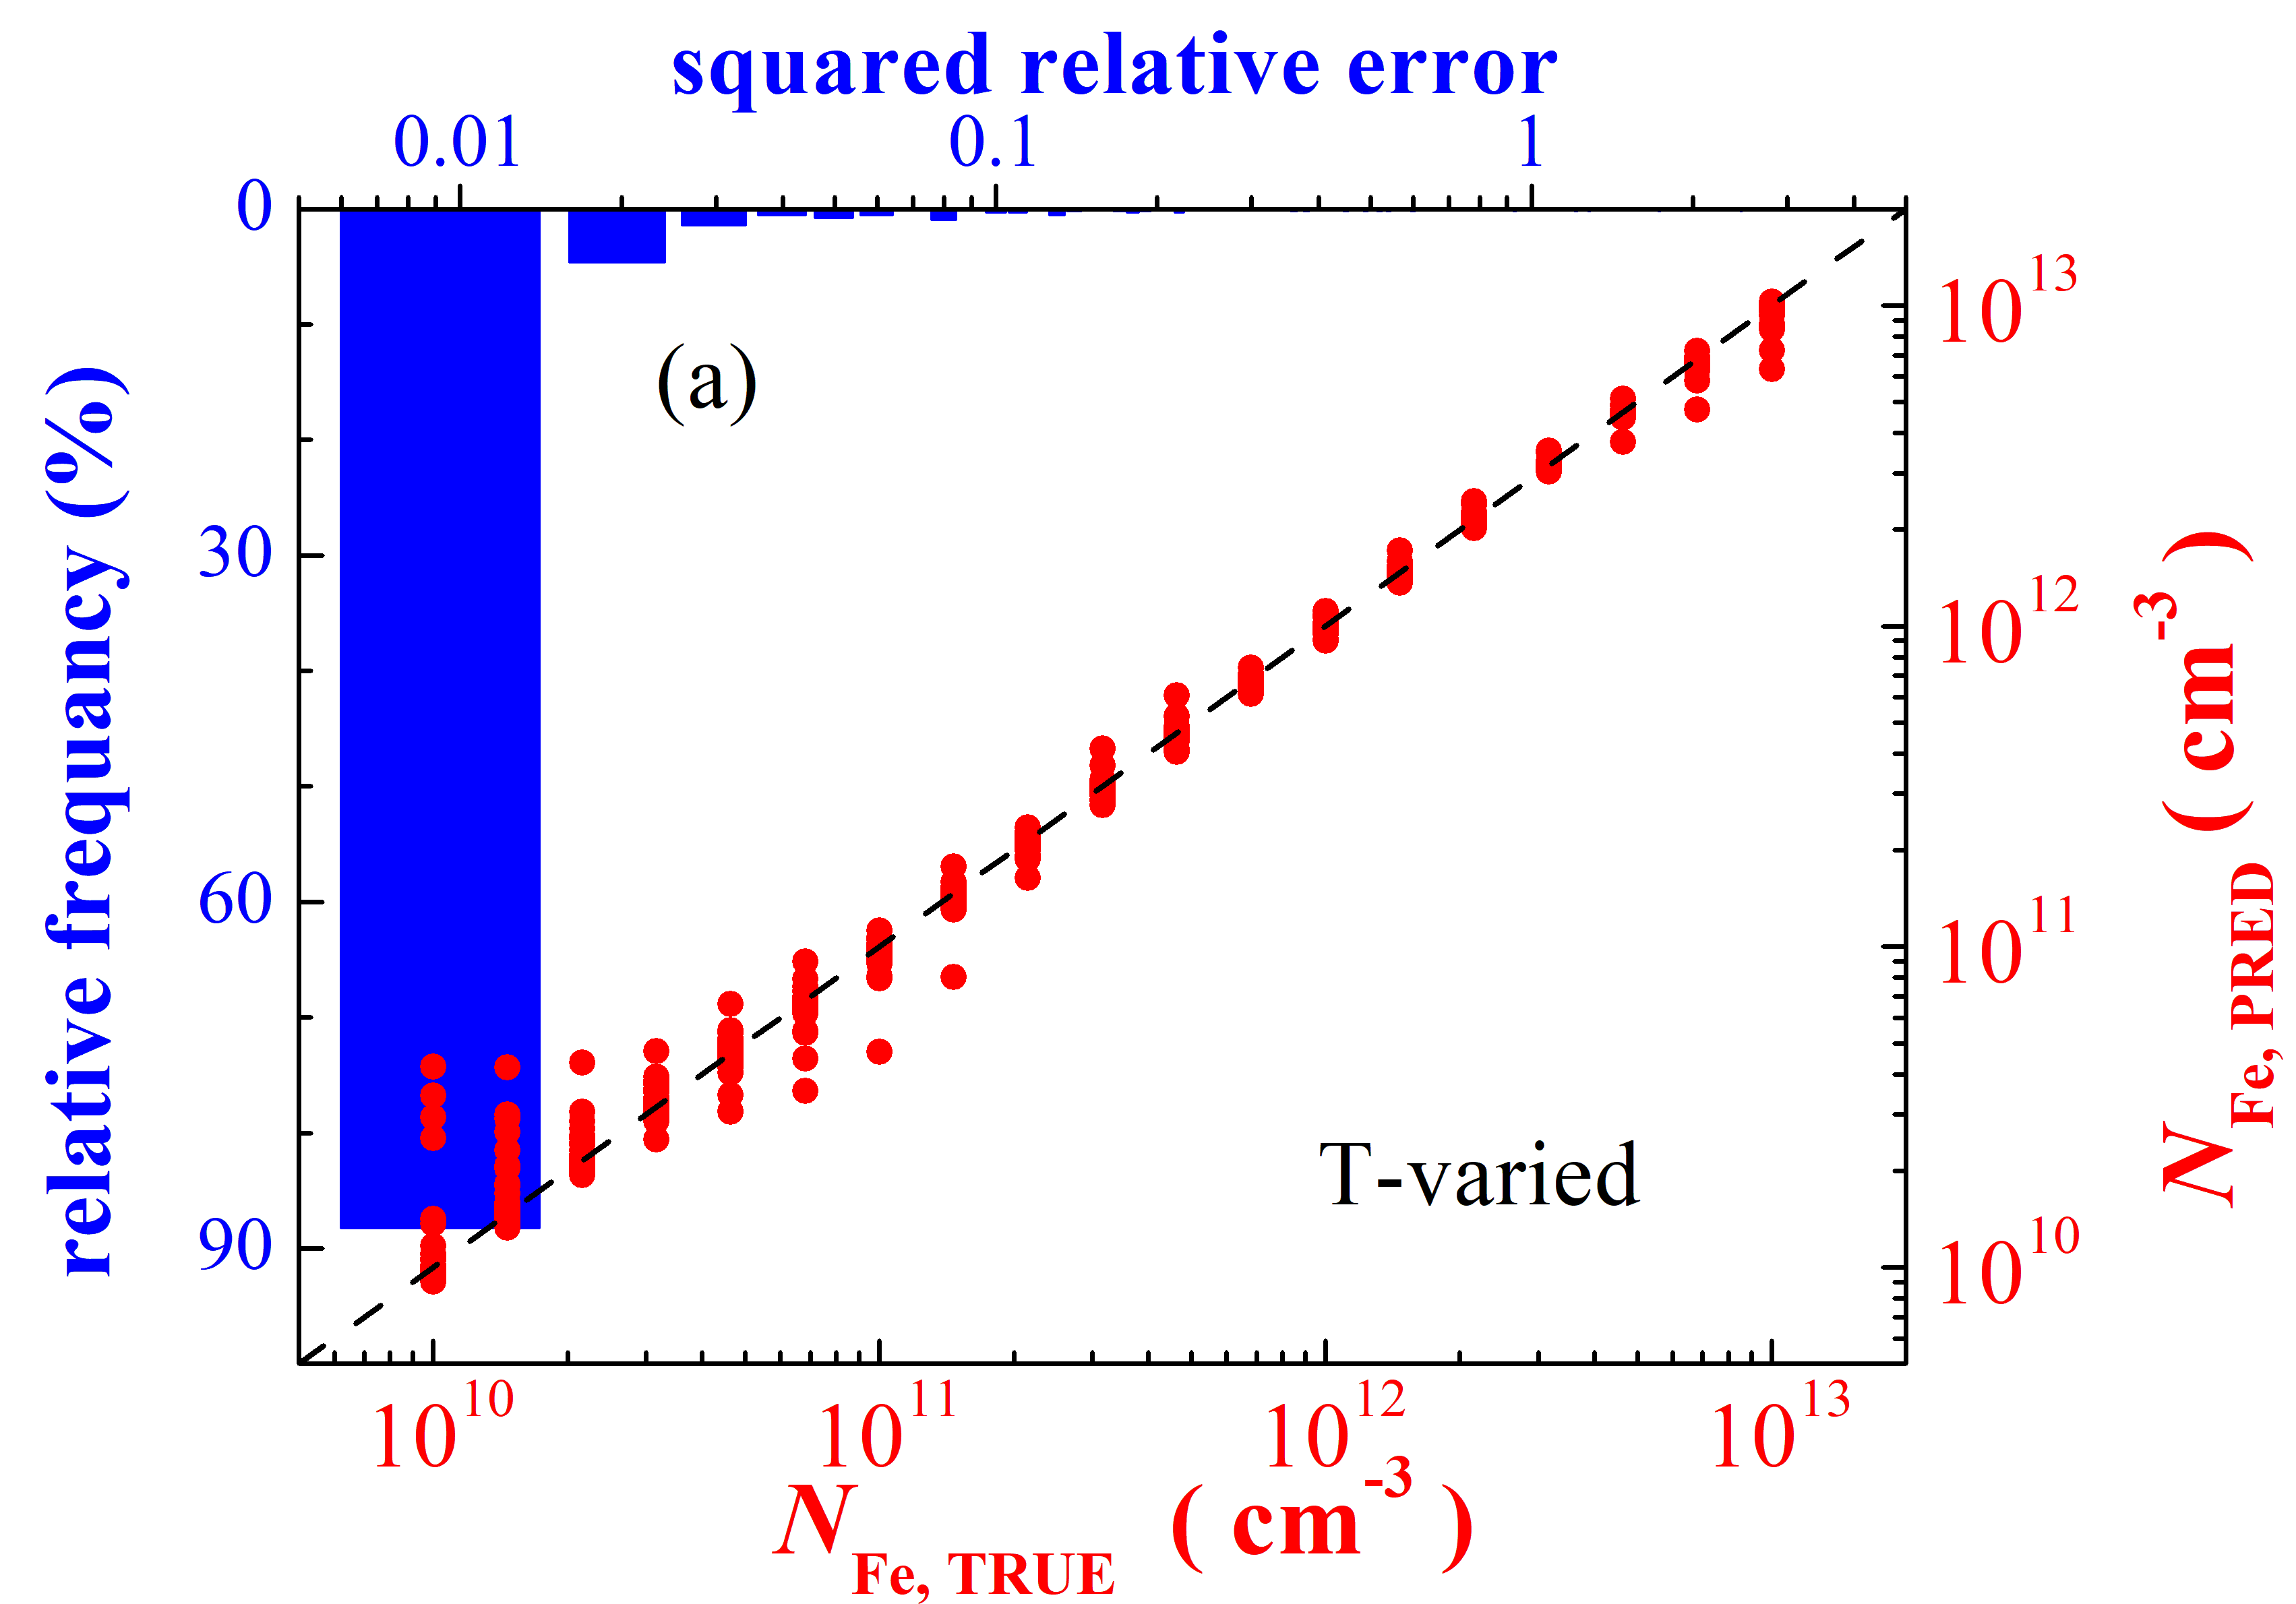
\includegraphics[width=0.32\textwidth]{F8a}
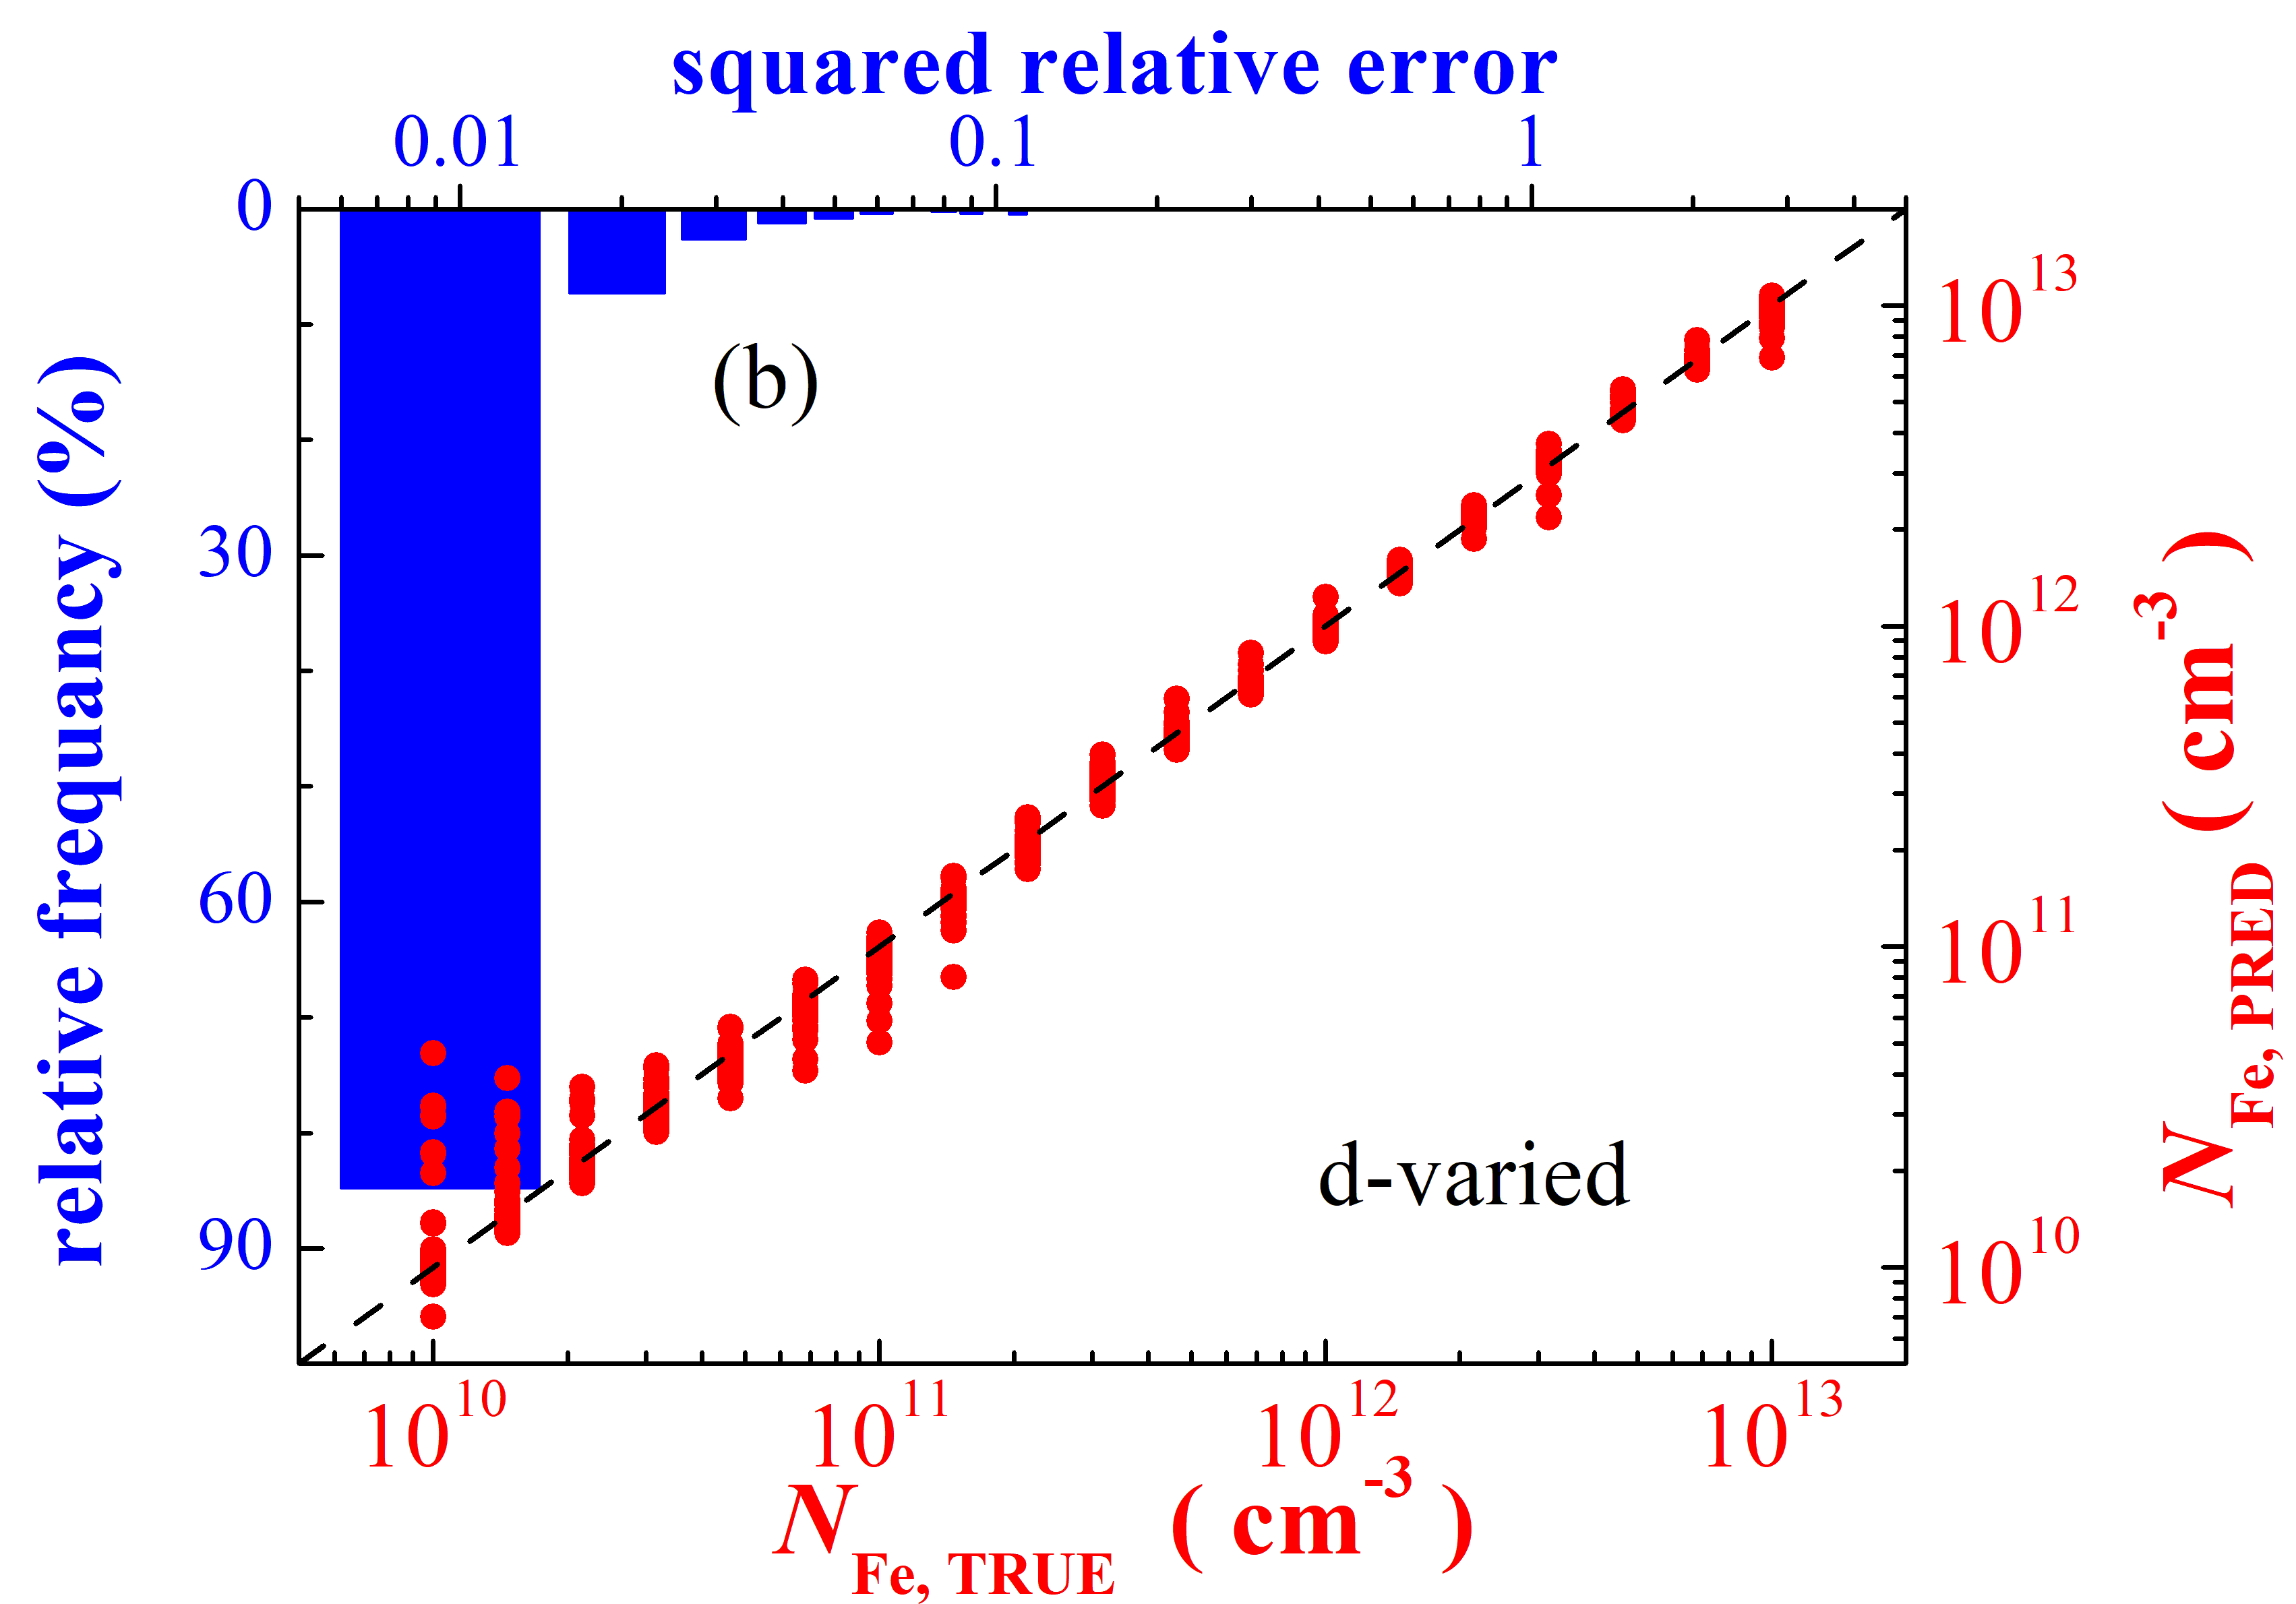
\includegraphics[width=0.32\textwidth]{F8b}
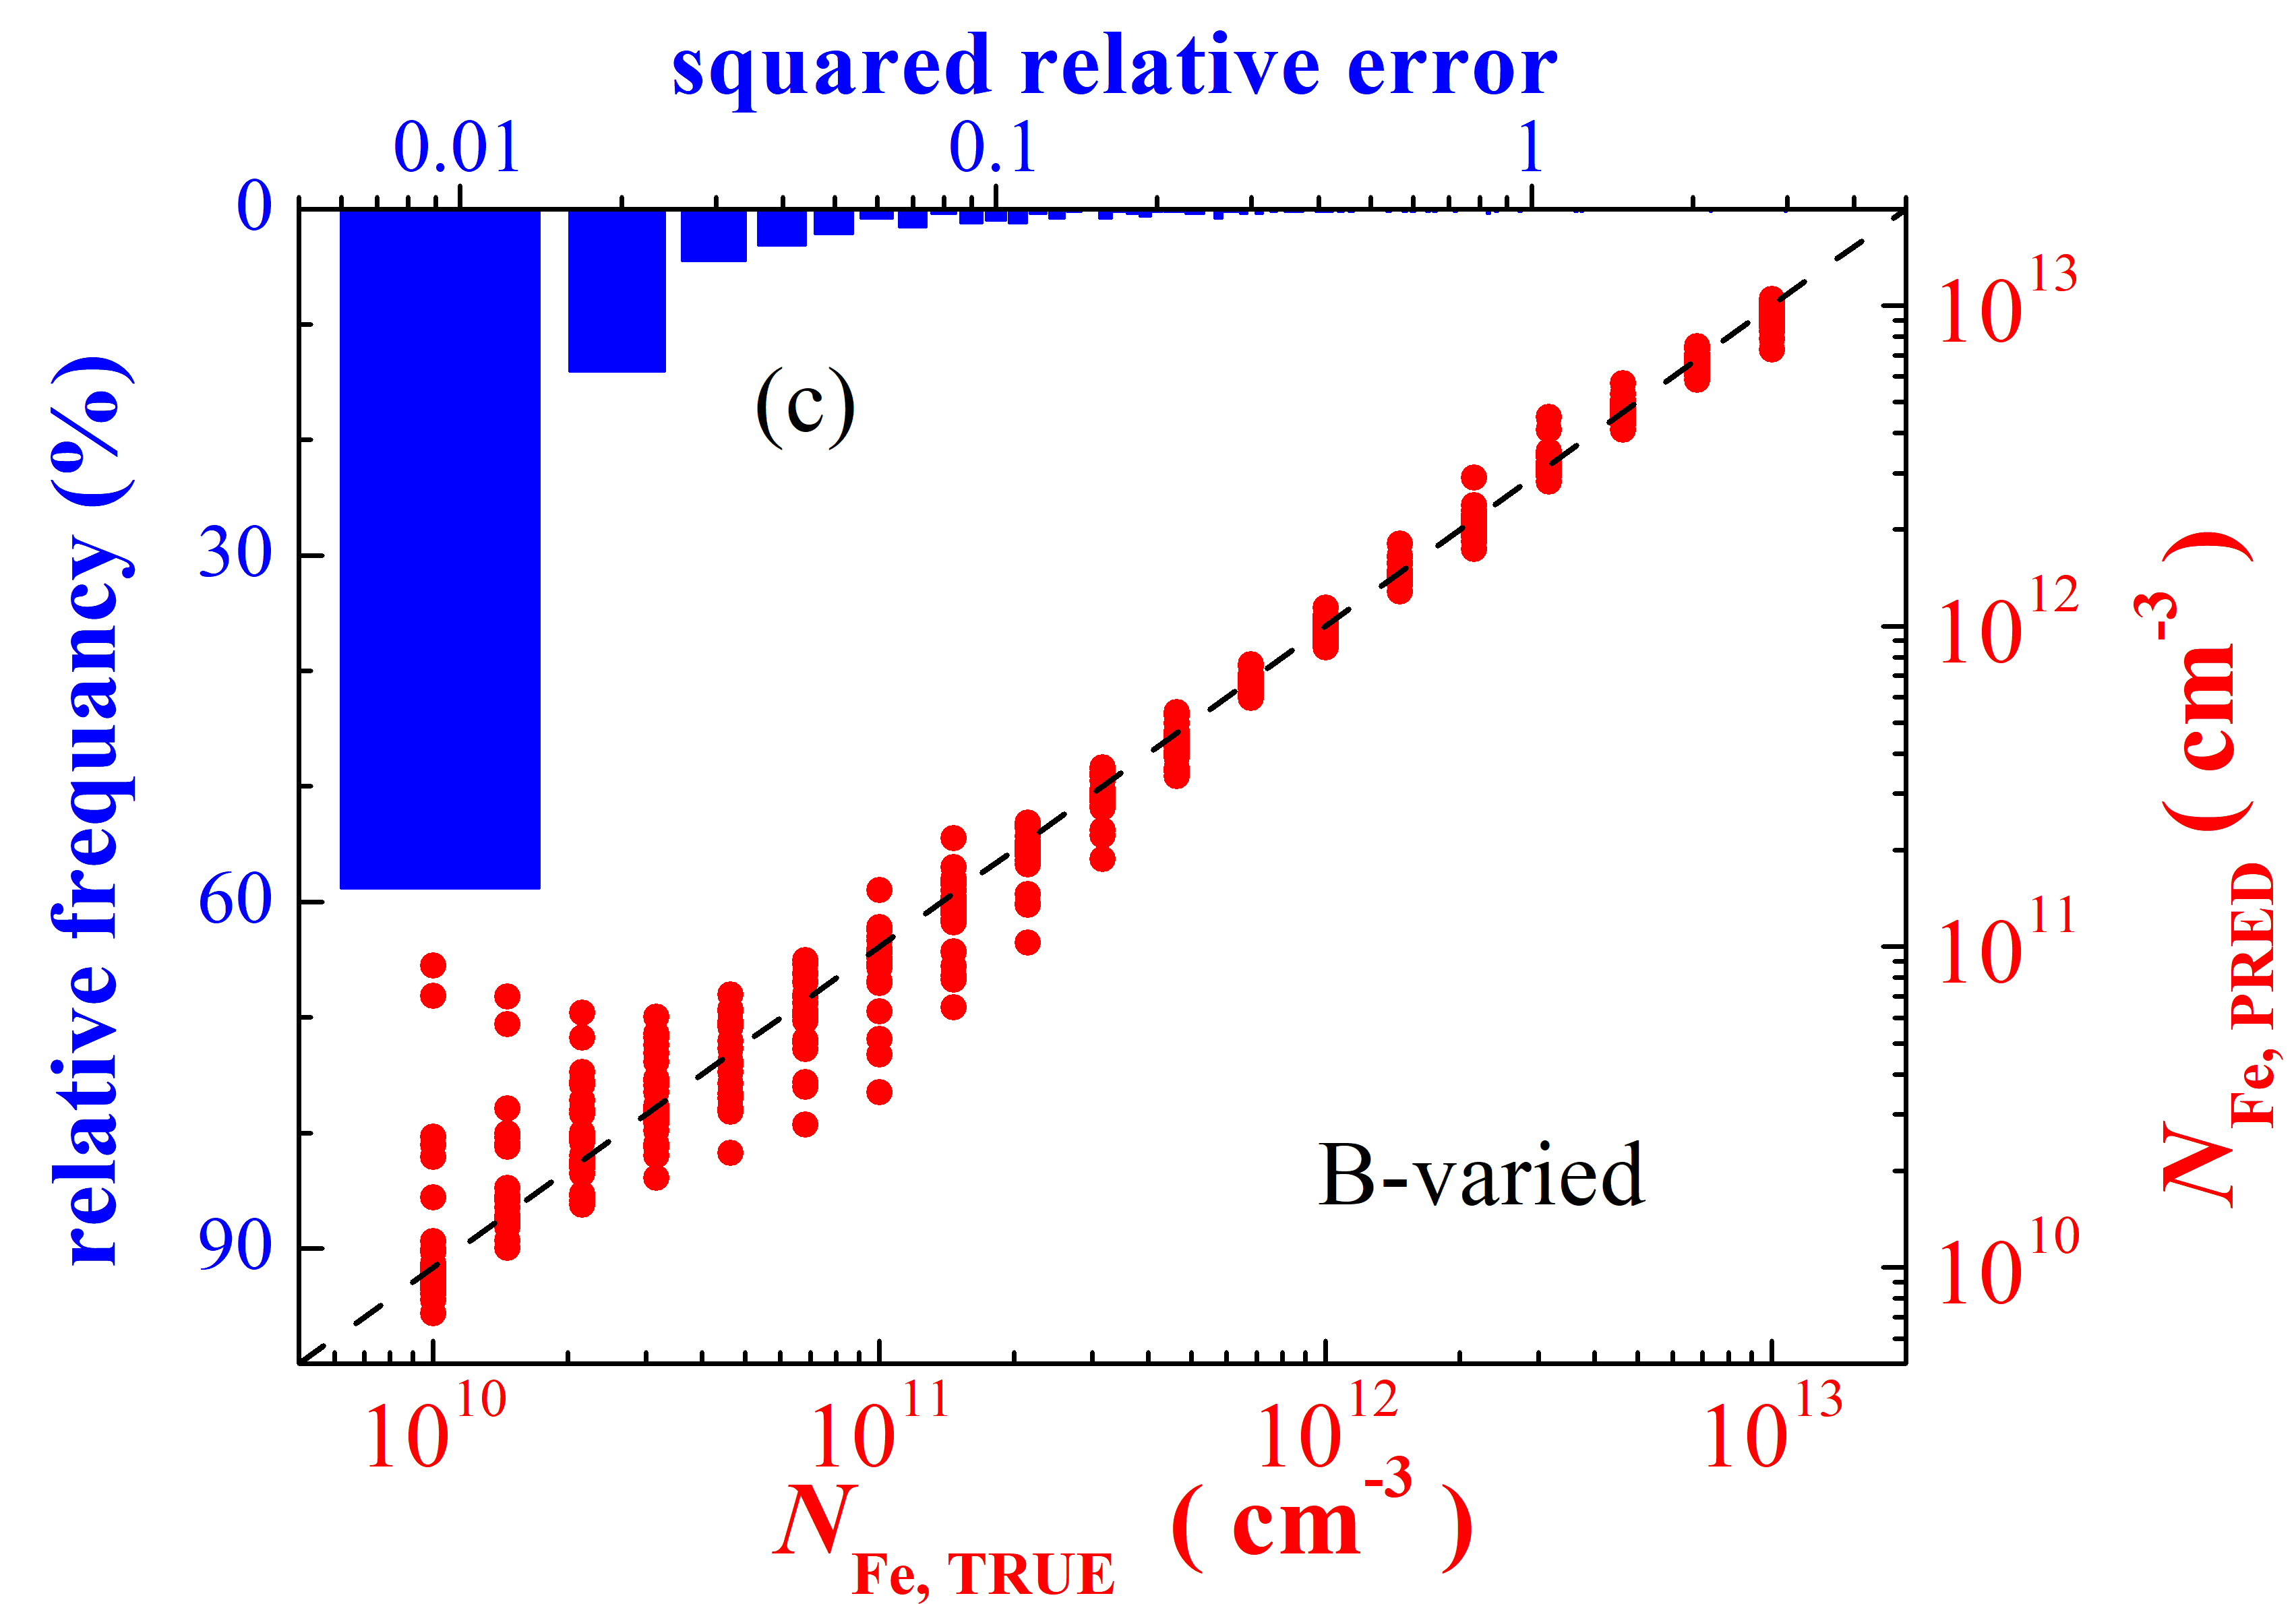
\includegraphics[width=0.32\textwidth]{F8c}
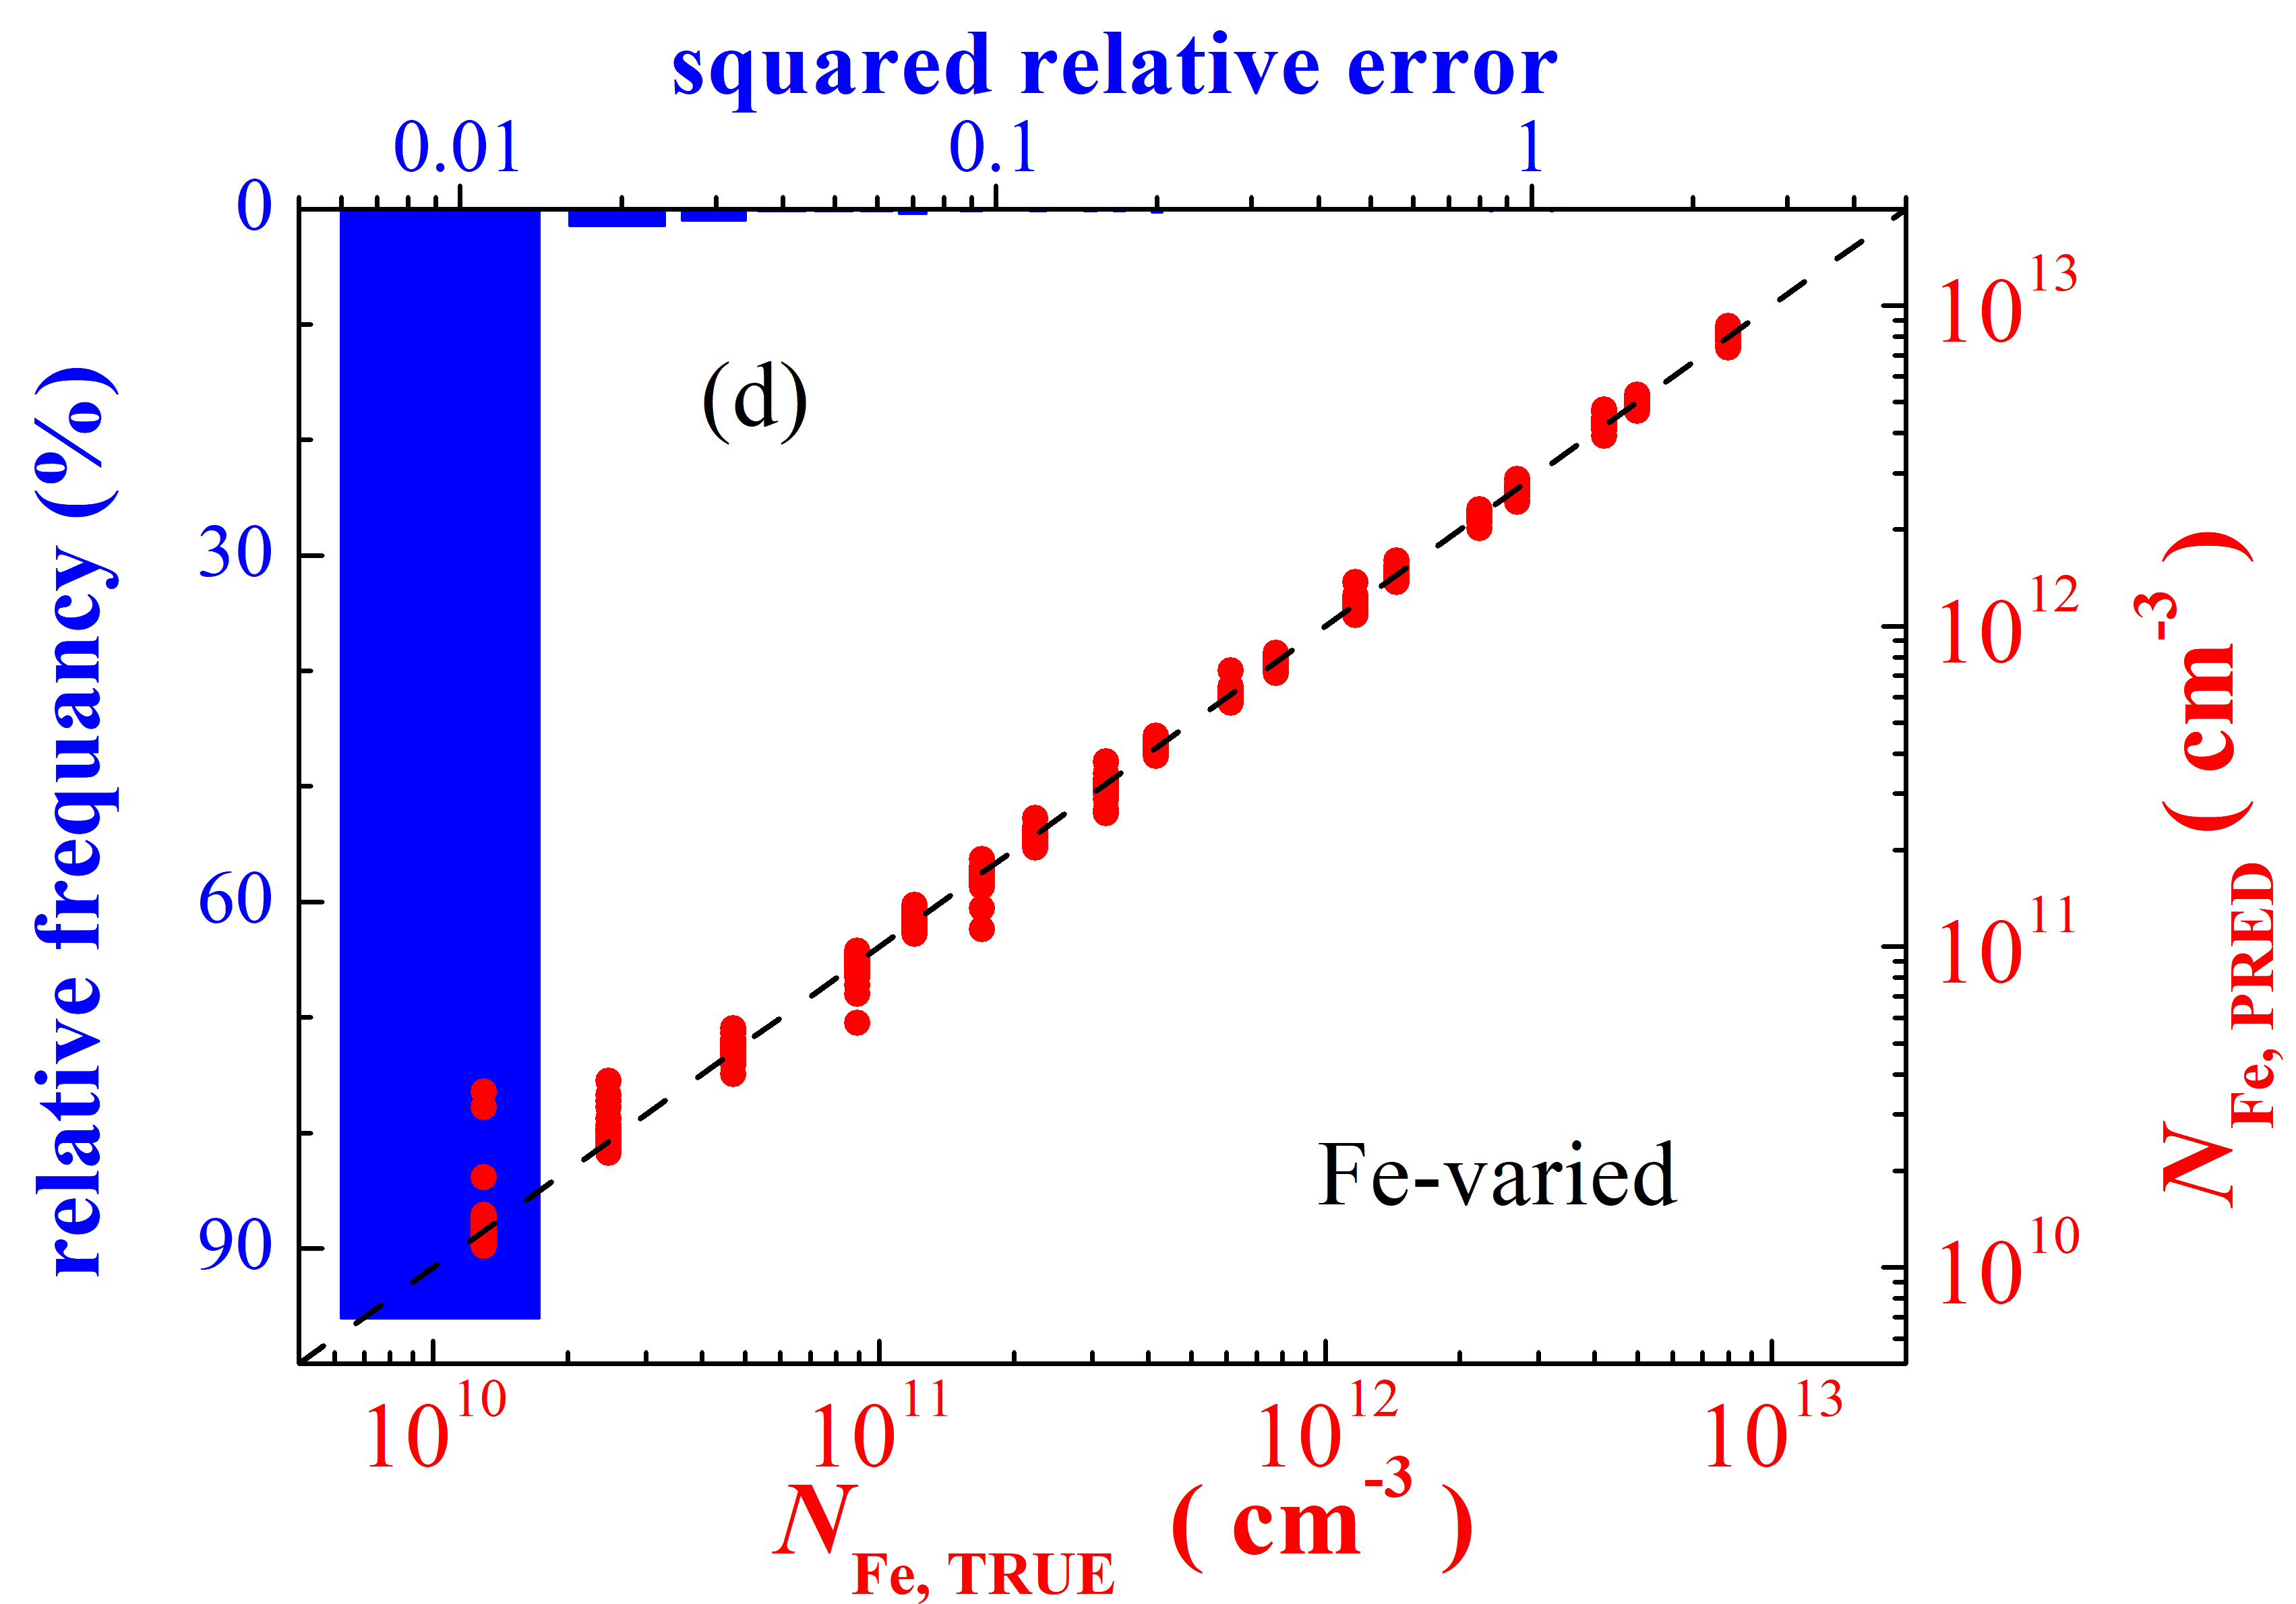
\includegraphics[width=0.32\textwidth]{F8d}
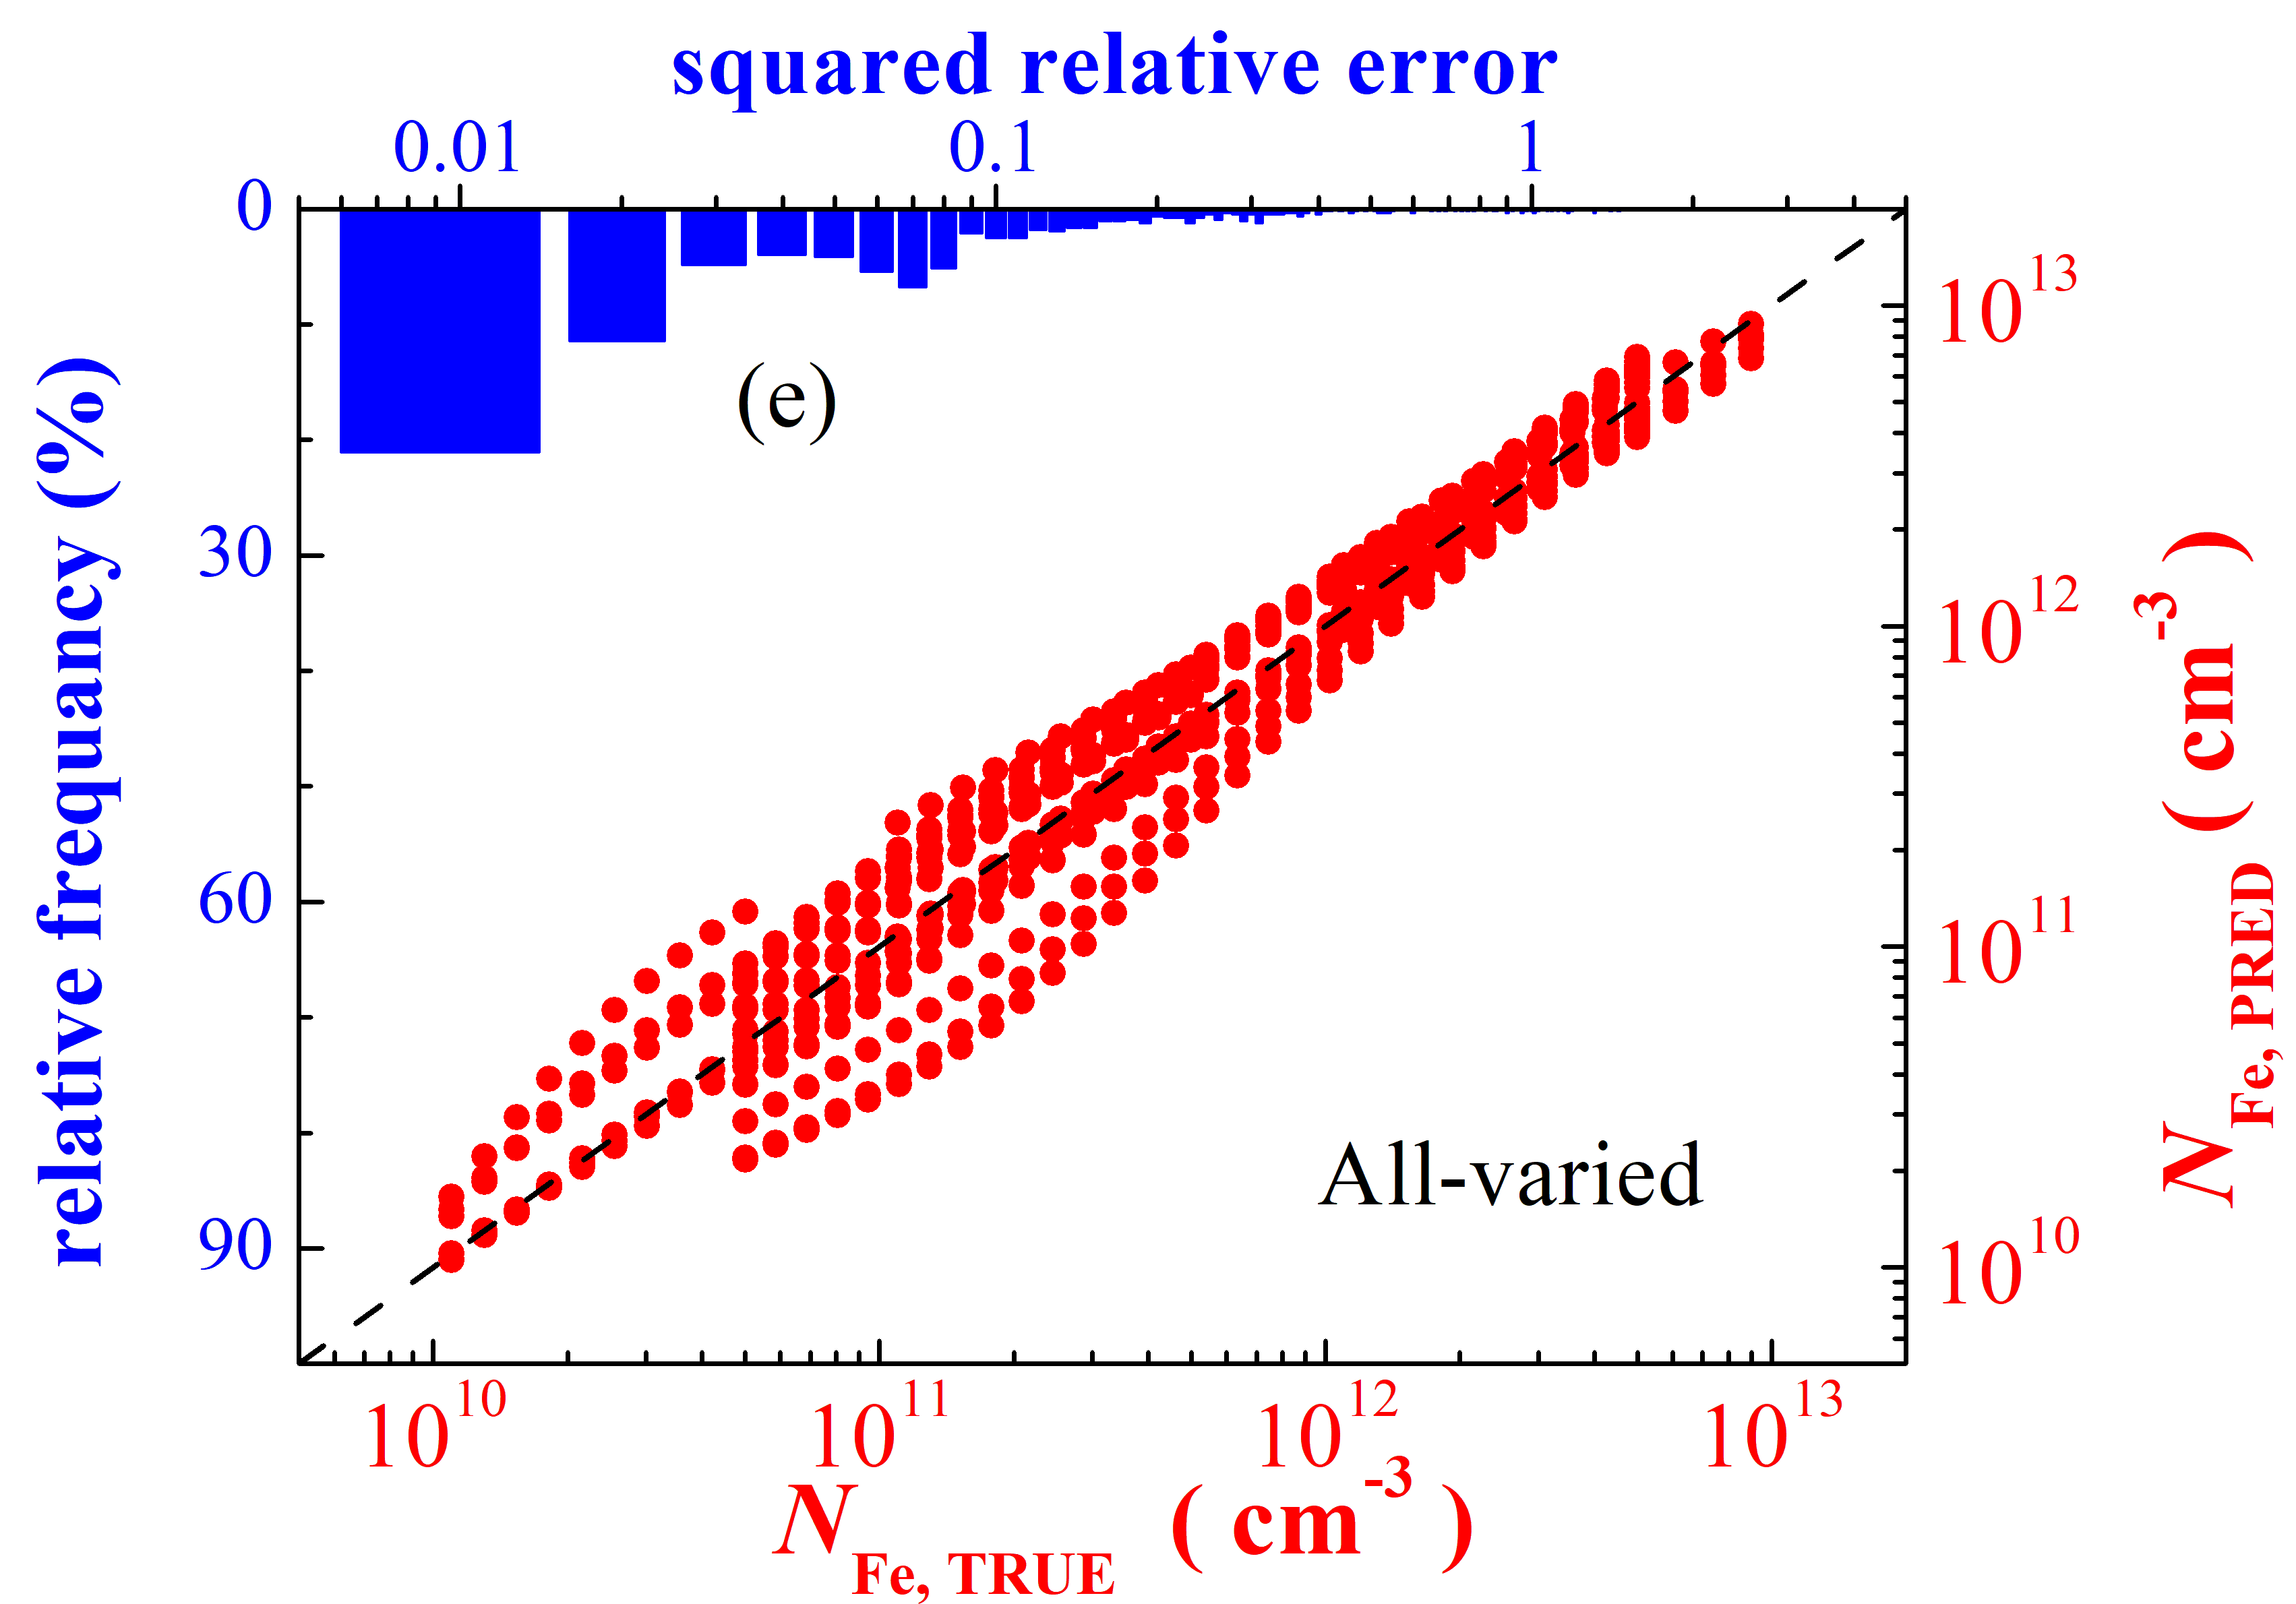
\includegraphics[width=0.32\textwidth]{F8e}
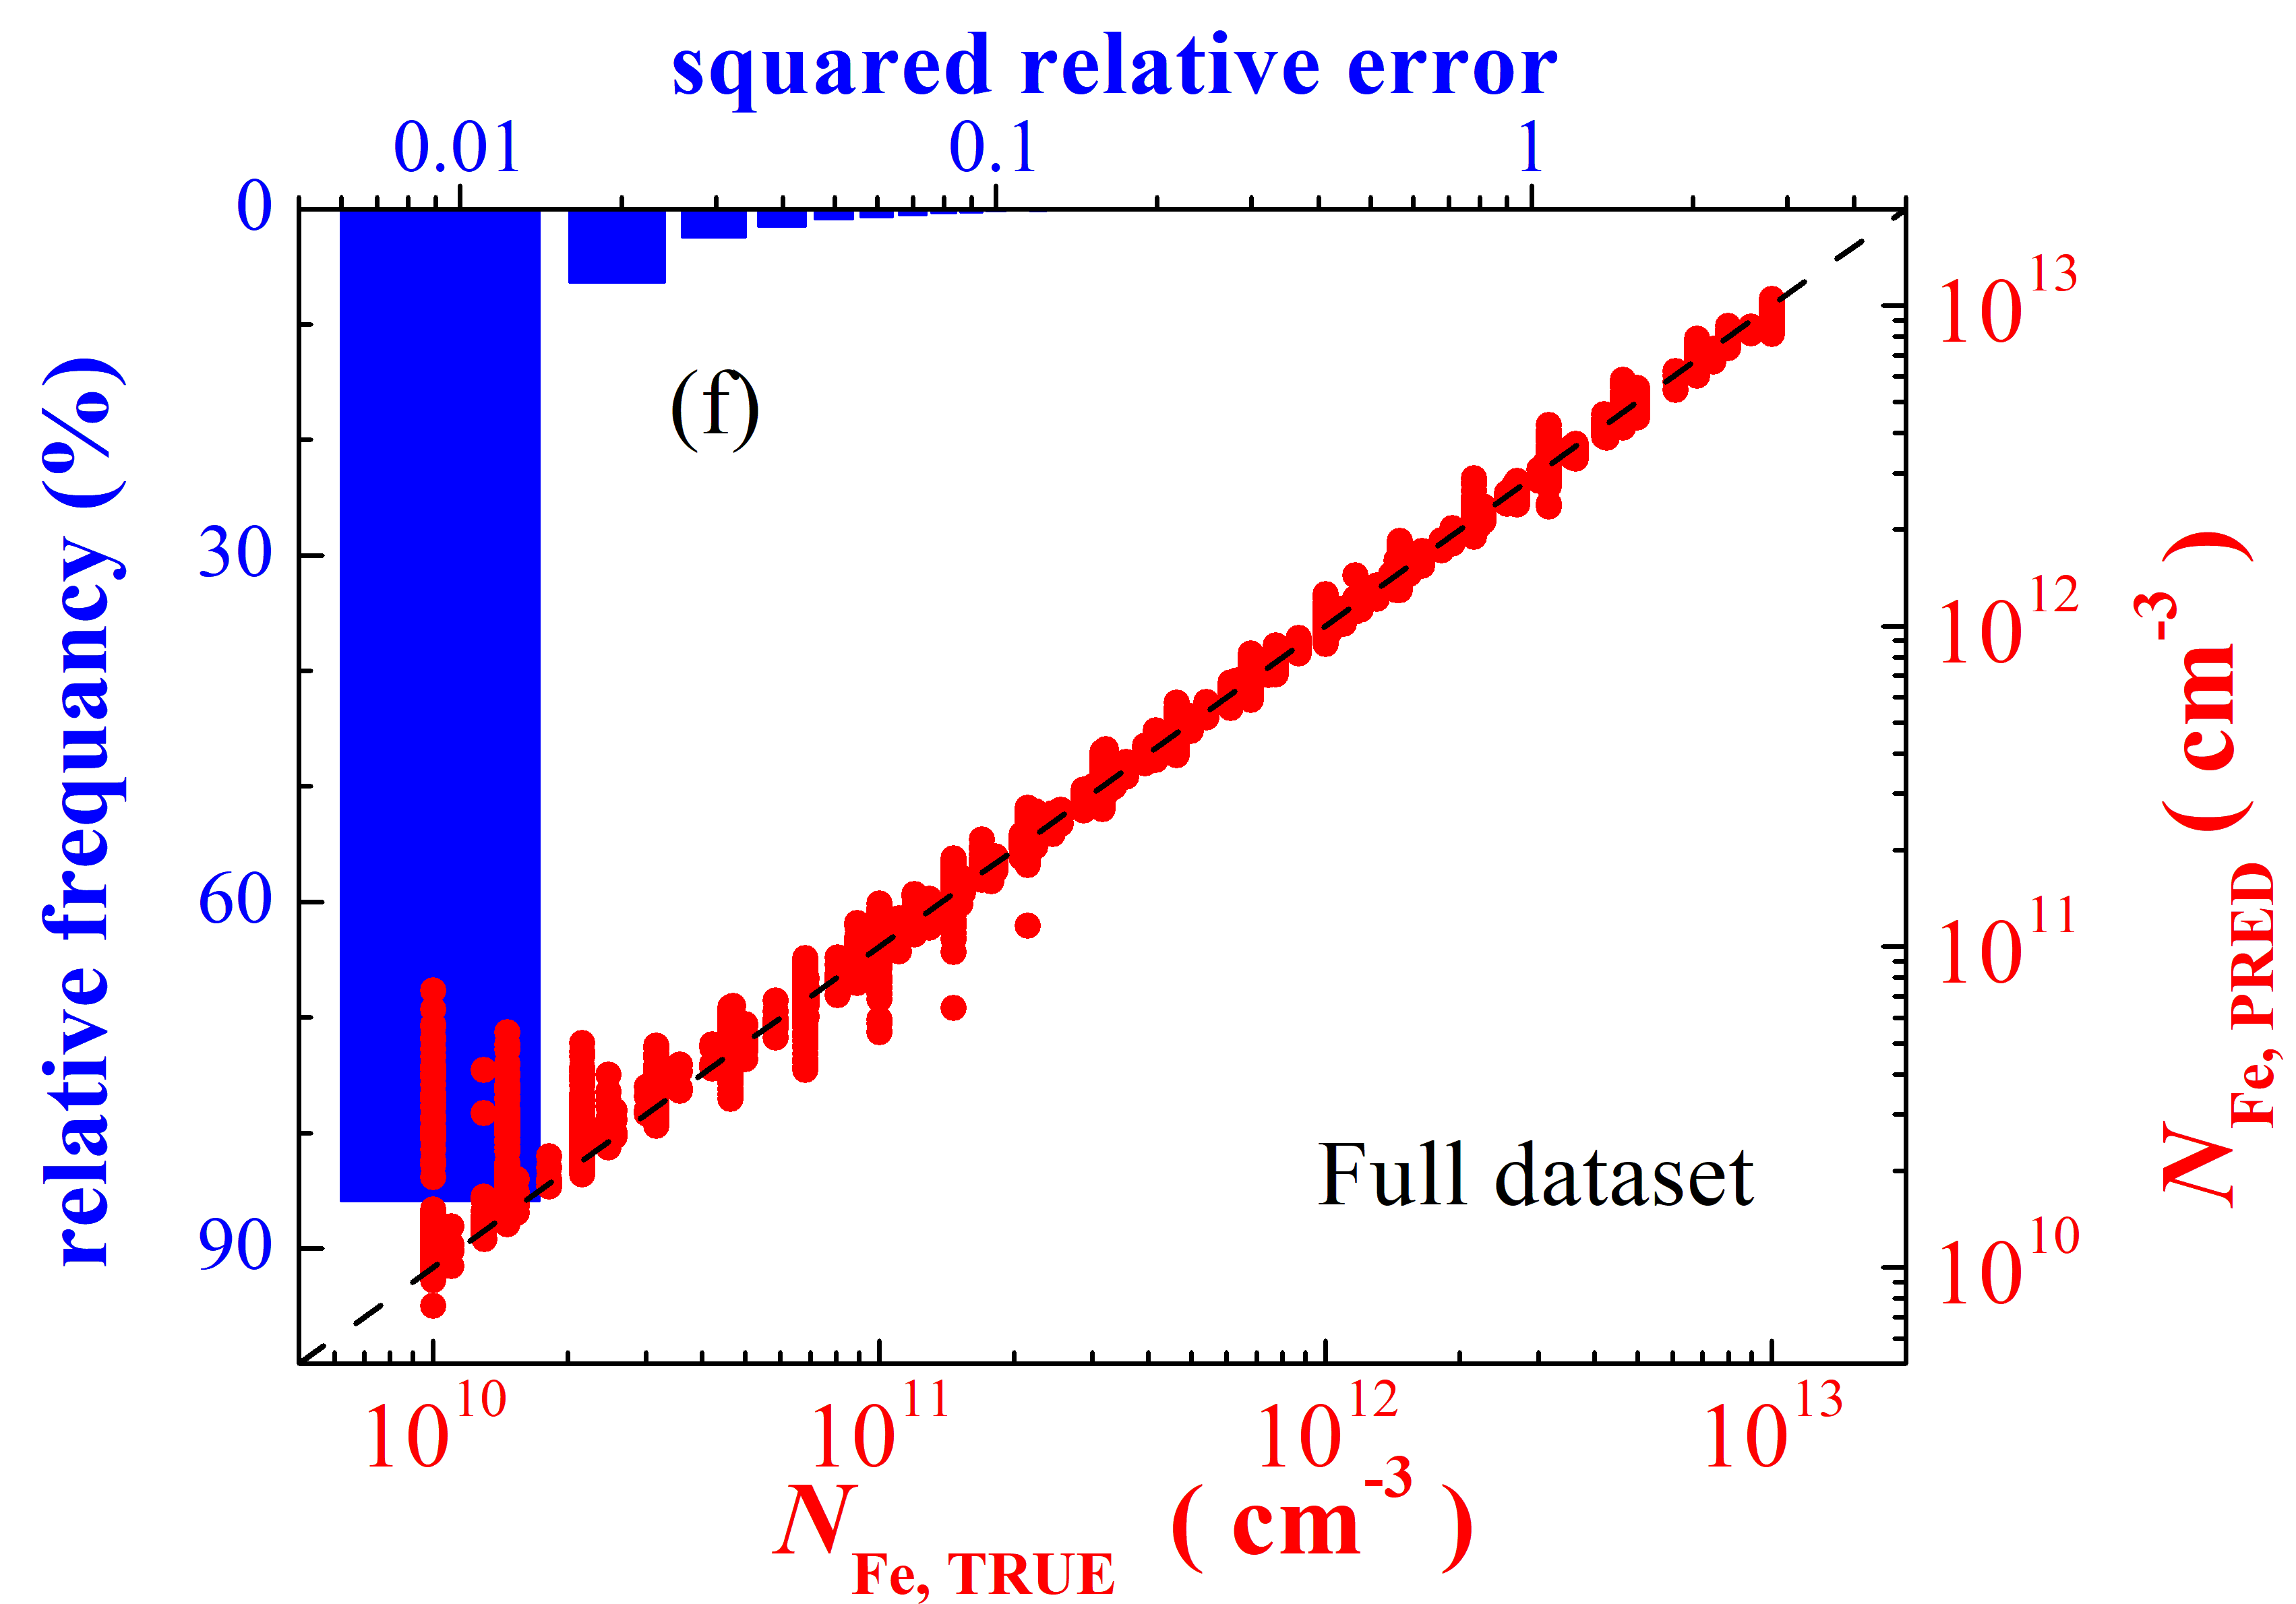
\includegraphics[width=0.32\textwidth]{F8f}
\caption{Iron concentrations are plotted against those generated by DNN$_\mathrm{FeFeB-Fe}$
on  T-varied (a),
d-varied (b),
B-varied (c),
Fe-varied (d),
All-varied (e),
and full (f) datasets (red points).
Bars represent histograms of squared relative error.
DNN was learned by training (a)--(e) or full (f) dataset.
The black dashed lines are the identify lines servings as the references.}
\label{fig_TrDNN2}
\end{figure}

Despite the difference in prediction accuracy,
the  features of DNN$_\mathrm{FeFeB-Fe}$ and DNN$_\mathrm{FeFeB}$ are similar.
Thus,
the DNN training with $N_\mathrm{B}$ values, which are expected to be an object of future research,
is important for the accuracy of prediction (Fig.~\ref{fig_TrDNN2});
the increase in the temperature (Fig.~\ref{fig_Temp}) as well as decrease
in doping level (Fig.~\ref{fig_B}) or iron concentration (Fig.~\ref{fig_Fe})
results in error increase.
It should be noted that the prediction error gain with $N_\mathrm{Fe}$ increase is not observed in case of DNN$_\mathrm{FeFeB-Fe}$ and
the range of SRE at $N_\mathrm{Fe}=10^{13}$~cm$^{-3}$ is narrower than that at $N_\mathrm{Fe}=10^{10}$~cm$^{-3}$ --- see Fig.~\ref{fig_Fe}(b,c).


The results of both DNN$_\mathrm{FeFeB}$ and DNN$_\mathrm{FeFeB-Fe}$
training with a full dataset are presented in Table~\ref{table_CV}, Fig.~\ref{fig_TrDNN1}(f), and Fig.~\ref{fig_TrDNN2}(f).
We can see that in our case the extension of the labeled dataset practically does not improve the result of DNN.
In our opinion, this is an evidence of
i)~good DNN configuration tuning;
ii)~restricted predictive ability of DNN$_\mathrm{FeFeB}$,
which is caused by ambiguity of dependence $n_\mathrm{Fe-FeB}=f(N_\mathrm{Fe})$.


\subsection{Experimental IV curves}


The ability of DNNs to predict iron concentration in real silicon SCs was tested as well.
The samples used in the experiment were $n^+$--$p$--$p^+$--Si structures.
The structures were fabricated from $p$--type boron doped Czochralski silicon wafer with [100]
orientation and resistivity of 10~Ohm$\cdot$cm ($N_B = 1.4\cdot10^{15}$~cm$^{-3}$).
The $n^+$ emitter with sheet resistance of about $(20\div30)$~$\Omega/\Box$ and a thickness
of $0.7$ $\mu$m was formed by phosphorus diffusion at 940$^\circ$;
$p^+$ layer ($(10\div20)$~$\Omega/\Box$, $0.6$~$\mu$m)
was formed by boron diffusion at 985$^\circ$C.
The base thickness was 350~$\mu$m.
The area of the samples was $1.52\times1.535$~cm$^2$.
The concentration of iron in the SC base $N_\mathrm{Fe,MEAS}$
was determined from kinetics of the short circuit current under monochromatic illumination \cite{2021CMLTP}.
Two samples used in the investigation are referred to as SC320 and SC349 with $N_\mathrm{Fe,MEAS}$
of $(2.0\pm0.4)\cdot10^{12}$~cm$^{-3}$ and $(6.7\pm0.7)\cdot10^{12}$~cm$^{-3}$,
respectively.

We can see that DNN was faced with a rather difficult task
when the complexity was associated with a certain mismatch between the parameters of real structures and those used in the simulation.
However, the need for iron-related defects, which predominantly determine recombination, was the main criterion for sampling in our case.


The dark IV characteristics of the samples were measured at temperatures
300, 320, and 340~K.
The measurements were carried out after 48~h exposition in the dark at room temperature
(``Fe-FeB'' case)
as well as immediately after intense illumination of the sample with a halogen lamp
(``Fe'' case).
To fit the experimental data and determine fitting parameters, in particular $n$, $R_s$, $R_{sh}$,
we used Eq.~(\ref{eqIVd}).
The typical results of the measurements and approximations are shown in Fig.~\ref{fig_IVexp}
and Table~\ref{table_Exp}.
It should be noted that for real IV curves, in contrast to synthetic ones,
the influence of series and shunt resistances cannot be neglected
(the magnitude of $R_s$ is about 3 and 6~Ohm for samples SC320 and SC349, respectively,
all the values of $R_{sh}$ are listed in Table~\ref{table_Exp}).

\begin{figure}[t]
\centering
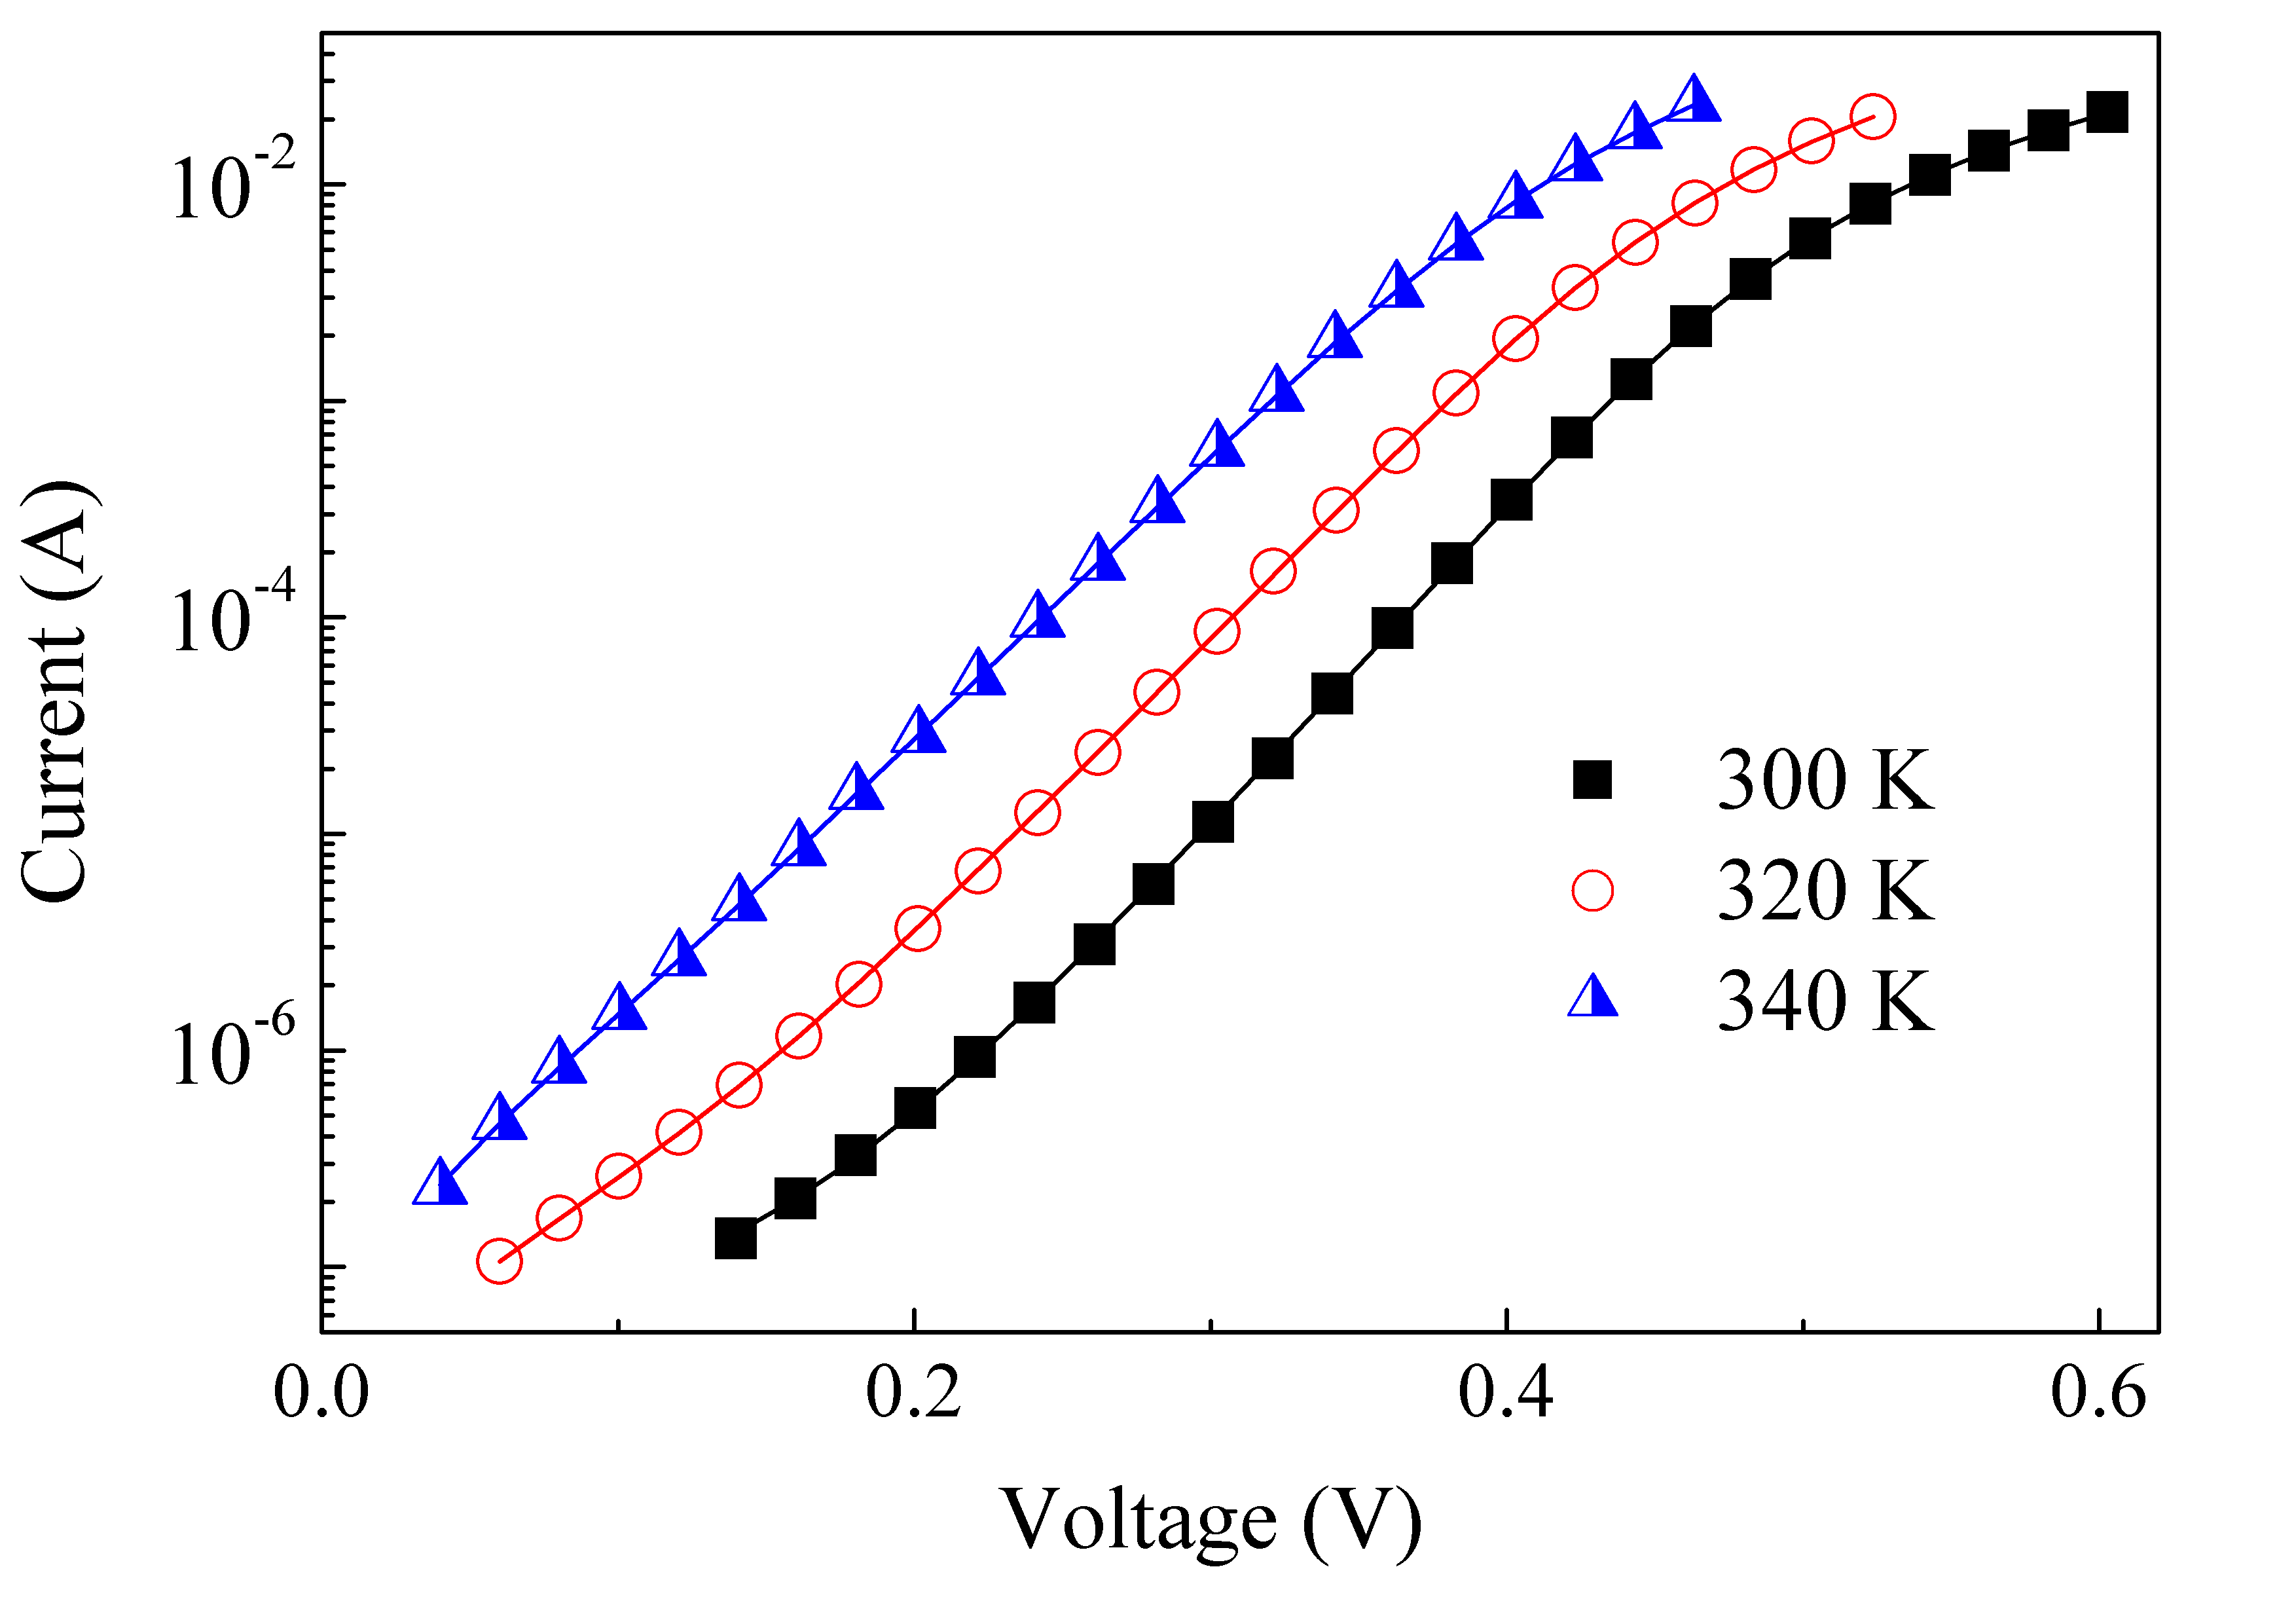
\includegraphics[width=0.5\textwidth]{F9}
\caption{
$I$–-$V$ characteristics measured at 300~K, 320~K, and 340~K for
sample SC320.
The marks are the experimental results, and
the solid lines are the curves fitted by
Eq.~(\ref{eqIVd}).
}
\label{fig_IVexp}
\end{figure}

\begin{table}
\caption{Results of experimental IV fitting and iron contamination testing}\label{table_Exp}
\begin{tabular}{lcccccccccc}%{\tblwidth}{@{} LLLLLLL@{} }
\headrow
\thead{Sample}&$N_\mathrm{Fe,MEAS}$, &$T$,&
$n_\mathrm{Fe-FeB}$&$R_{sh,\mathrm{Fe-FeB}}$,&
$n_\mathrm{Fe}$&$R_{sh,\mathrm{Fe}}$,&
\multicolumn{4}{c}{$N_\mathrm{Fe,PRED}$, $10^{12}$~cm$^{-3}$}\\
\headrow
&$10^{12}$~cm$^{-3}$&K&&Ohm&&Ohm&\multicolumn{2}{c}{DNN$_\mathrm{FeFeB}$}&\multicolumn{2}{c}{DNN$_\mathrm{FeFeB-Fe}$}\\
\headrow
&&&&&&&training&full&training&full\\
SC320&$2.0\pm0.4$&300&1.214&$1.6\cdot10^6$&1.195&$1.4\cdot10^6$&3.9&2.8&3.0&2.0\\
&&320&1.204&$8.6\cdot10^5$&1.148&$8.0\cdot10^5$&6.6&1.9&16&19\\
&&340&1.118&$4.3\cdot10^5$&1.111&$4.3\cdot10^5$&3.8&1.2&89&574\\
SC349&$6.7\pm0.7$&300&1.223&$2.9\cdot10^6$&1.222&$2.6\cdot10^6$&8.9&5.6&15&11\\
&&320&1.183&$1.7\cdot10^6$&1.182&$1.7\cdot10^6$&1.2&0.4&10&32\\
&&340&1.138&$1.3\cdot10^6$&1.173&$1.3\cdot10^6$&9.8&1.7&26&411\\
\hline
\end{tabular}
\end{table}

The ideality factors determined from the experimental curves
and the sample parameters were used as input data for
DNN$_\mathrm{FeFeB}$ and DNN$_\mathrm{FeFeB-Fe}$,
which were trained  either on the training dataset or full dataset.
The predictions are listed in Table~\ref{table_Exp}.

First of all, it should be noted that
even though we did not use a simulation model of extremely high complexity,
the results exceeded our expectations.
In particular, the predicted iron concentrations in DNN$_\mathrm{FeFeB}$
differed only several times from the measured ones.
In the case of sample SC320 and DNN$_\mathrm{FeFeB}$ trained on the full dataset,
the error did not exceed 40\%.

Also, it should be noted that the results confirm
the trends revealed  by the analysis of synthetic IV curves.
In particular, the prediction accuracy decreases at $T>320$~K
and iron concentrations close to the upper limit in the range ($10^{13}$~cm$^{-3}$).
These facts completely coincide with the data in Fig.~\ref{fig_Temp}a and Fig.~\ref{fig_Fe}a, respectively.
In addition, the sample's base doping level ($N_B=1.4\cdot10^{15}$~cm$^{-3}$) is not used in the training dataset
but can be found in the d--varied dataset (see Supplementary Material).
Table~\ref{table_Exp} shows that the prediction of DNN$_\mathrm{FeFeB}$
trained by a full dataset is better than in the case of learning only by a training dataset, especially for SC320 sample.
This fact confirms the conclusion made in the previous section about the importance of DNN training with $N_B$ values,
which are expected to be the object of future research.




On the other hand, contrary to our expectations, DNN$_\mathrm{FeFeB-Fe}$ demonstrates worse performance
than DNN$_\mathrm{FeFeB}$ in the majority case.
The likely reasons are the following.
First, the use of two ideality factor values makes the influence of simulation simplifications more significant
(e.g., the effect of unaccounted processes that cause both shunt and series resistance).
Secondly, to obtain a correct $n_\mathrm{Fe}$ is a more complicated experimental task than to determine $n_\mathrm{Fe-FeB}$.
For example, in our experiment it took about 100~s to obtain IV characteristics after intense illumination.
This interval included the time required to set the temperature after illumination-induced heating and the time of measurement.
According to \cite{FeBAssJAP2014,FeBKin2019}, the characteristic association time of FeB pairs
at $T=340$~K and $N_B=1.4\cdot10^{15}$~cm$^{-3}$ is about 600~s.
That is, despite the potentially higher accuracy of the DNN$_\mathrm{FeFeB-Fe}$ predictions
(shown in the previous section), the practical application of this approach is more complicated.

On the whole, the results obtained for real SCs confirm the possibility to estimate iron contamination using the ideality factor.

Finally, we would like to suggest some speculations about the applicability of the trained DNNs to different SC structures.
The speculations are based on assumption that the ideality factor distinguishes
depletion-region recombination from most other sources of recombination \cite{Breitenstein2013,n2McIntosh}.
Certainly, there are some deviations from this rule for real structures.
For instance, our simulation reveals the $n$ dependence on base thickness \cite{OlikhJPS}.
Nevertheless this dependence is weak, and the ideality factor value is mainly determined
by depletion-region recombination.


First of all, the DNNs applicability depends on the requirement for Shockley–Read–Hall recombinationto be predominant.
In case,
if there are other mechanisms causing free carrier concentration to decrease,
the models which diverge from the two-diode one are proposed
(e.g., three-diode \cite{TreeDiode,Shah}).
Moreover, the base must be doped by boron.
For example, if SC is prepared from Si:Al wafer,
the simulation model which is used for training dataset preparation must be modified:
the parameters of $\mathrm{Fe}_i\mathrm{Al}_s$ pair as well as
the changes in defect distribution (Eq.~(\ref{eqNFeB})) should be taken into consideration.
Finally, if another type of defect (in addition to iron--related deep levels)
is present in the solar cell, which also induces intensive SRH recombination,
the simulation model must be more complicated as well.
The primary competitors of $\mathrm{Fe}_i\mathrm{B}_s$  are  boron-oxygen complexes \cite{LIDRev,LIDRev2}
and oxide precipitates \cite{MurphySC2014,Oxide:Chen} in Cz-Si.
So the development of the corresponding model can be our next step.
To the point, it should be noted that a high $n$ value can serve an indicator of another defect presence:
in our simulation this value is $n<1.4$.
The absence of non-iron active defects may be the most limiting factor of the DNNs applicability;
in particular, this confined the selection of SCs for our experimental verification of the proposed method.


Thus, the trained DNNs can be applied to BSF solar cells prepared from Si:B wafers.
It should be noted that the modern  technique of crystal growth
makes it possible to restrict
oxygen concentration substantially even in solar grade Cz-Si.
On the one hand,  Al is used to produce the doped $p^+$ region
at the industrial level \cite{GreenRew2019,WilsonRew2020}.
However, since a boron BSF is one of the promising techniques
for achieving high quality back contact \cite{Kim2007,B-BSF}
therefore the $p^{+}$ layer, which is doped by boron, was under our consideration.
On the other hand, 
he probable $p^+$--layer influences this process mostly via the electric field.
Therefore, the kind of doping atom in $p^+$--layer is not very important for simulation,
and in our opinion, the  DNNs is applicable for Al BSF cell as well.
Besides, the recombination in the rear surface region is not crucially important for estimating the ideality factor.
The wake aforesaid allows us to make a conclusion that
the trained DNN can be applied to those PERC solar cell in which
i)~the base is boron-doped;
ii)~the iron-related deep levels are the main cause of defect-assisted recombination.




\section{Conclusion and Outlook}

In this paper,
we determined iron concentration in silicon BSF solar cells from
the ideality factor value and systematically studied the performance
of deep learning for the indicated task.
It was  the first attempt to use deep learning for retrieving deep level parameters from the current--voltage curve.
In the model study,
we performed simulation in order to obtain a training labeled dataset and test labeled datasets.
In the end, DNN was trial-tested by using the parameters of actual solar cells.
Our results showed the DNN ability
to predict iron concentration by ideality factor,
thickness and doping level of SC base as well as temperature.
For synthetic datasets the MSRE was as small as 0.005.
Our simulation shows the prospects for applying the ideality factor of two values (for structure with $\mathrm{Fe}_i$ only as well as with $\mathrm{Fe}_i\mathrm{B}_s$ and
$\mathrm{Fe}_i$ coexistence)
in order to upgrade prediction accuracy.
At the same time, the practical application of this approach demonstrated difficulties in obtaining correct data.
It was important to train the DNN with boron concentration values,
which agreed with the doping level of the structures under study.
Moreover, the increase in iron or boron concentration, as well as temperature decrease,
resulted in smaller prediction errors.

The proposed approach uses a simple and widely applied setup and does not take much time.
Therefore, it could be easily integrated into the manufacturing environment.
It should be noted, however, that for our purposes the task was  simplified.
Nevertheless, we believe that this DNN approach can be further improved in two ways.
The first is to refine labeled datasets by using 3D-simulators (e.g., SILVACO TCAD) or real IV measurements in a broad set of SCs.
The second is to improve DNN operation, and fine-tuning seems to be most promising in this case.
For example,
innumerous input parameters can be multiplied and transformed into a picture
so that the vision model (e.g., VGG16) could be applied.



\section*{Acknowledgments}
This work was supported by National Research Foundation  of Ukraine
(project number 2020.02/0036)

\section*{Conflict of Interest}
The authors declare that they have no known competing financial interests or
personal relationships that could have appeared to influence the work reported
in this paper.
%You may be asked to provide a conflict of interest statement during the submission process. Please check the journal's author guidelines for details on what to include in this section. Please ensure you liaise with all co-authors to confirm agreement with the final statement.

\section*{Data availability}

The simulated IV characteristics, $n_\mathrm{Fe}$ and $n_\mathrm{Fe-FeB}$ values,
and trained DNNs are available
at \newline
\emph{https://github.com/olegolikh/IVcharacteristics.git}.

%\section*{Supporting Information}
%Supporting information is information that is not essential to the article, but provides greater depth and background. It is hosted online and appears without editing or typesetting. It may include tables, figures, videos, datasets, etc. More information can be found in the journal's author guidelines or at \url{http://www.wileyauthors.com/suppinfoFAQs}. Note: if data, scripts, or other artefacts used to generate the analyses presented in the paper are available via a publicly available data repository, authors should include a reference to the location of the material within their paper.


\bibliographystyle{rss}
%\bibliographystyle{WileyNJD-Harvard}
\bibliography{olikh}

%\begin{biography}[example-image-1x1]{F. Author}
%Please check with the journal's author guidelines whether author biographies are required. They are usually only included for review-type articles, and typically require photos and brief biographies (up to 75 words) for each author.
%\bigskip
%\bigskip
%\end{biography}
%
%\graphicalabstract{example-image-1x1}{Please check the journal's author guidelines for whether a graphical abstract, key points, new findings, or other items are required for display in the Table of Contents.}

\end{document}
